\documentclass[11pt,aps,preprint,nofootinbib,superscriptaddress,tightenlines]{revtex4-2}
\usepackage{amsmath,amssymb,bm,mathtools}
\usepackage{graphicx}
\usepackage{xcolor}
\usepackage{algpseudocode}
\usepackage{dsfont}
\newcommand{\one}{\mathds{1}}
\newcommand{\pf}{\bm{\mathsf p}}
\newcommand{\avg}[1]{\langle #1\rangle}
\definecolor{darkblue}{RGB}{0,0,160}
\usepackage[colorlinks=true,linkcolor=darkblue,citecolor=darkblue,urlcolor=darkblue]{hyperref}

\def\st{\begin{equation}}
\def\stp{\end{equation}}
\def\Eq#1{eq.~(\ref{#1})}
\def\Sect#1{Sect.~\ref{#1}}
\def\Fig#1{Fig.~\ref{#1}}
\def\tr{\operatorname{tr}}
\let\oldparagraph\paragraph
\renewcommand{\paragraph}{\par\bigskip\oldparagraph}

\begin{document}

\title{The dissipative step with inverse-moment faces: plan}
\author{D.~Teaney}
\affiliation{Department of Physics and Astronomy, Stony Brook University,
Stony Brook, New York 11794, USA}
\date{\today}

\begin{abstract}
The common scheme (\texttt{commonkernel.tex}) corrects the bond weights of every star by a matrix $\Lambda_a$ so that its bond moment
is isotropic, and subtracts the virial of the residual draws through the faces.  We propose to handle the shape of each star instead
by inverting its bond moment: the faces carry the inverse moment, and the residual move is a Gaussian conditioned on zero virial.
$\Lambda_a$ is then not needed, the closure of the faces holds for any star, and the residual is the least-squares residual of the bond
differences, so the deterministic step needs no extra term.  With fixed faces both moves have closed-form proposal densities, and the
Hastings correction removes the bias of rebuilding the coefficients, which is up to $14\%$ at $s_a=16$.  This note is the plan; nothing
is implemented.
\end{abstract}

\maketitle

\noindent\emph{The runs reported here are before the branch \texttt{dimfix} (\texttt{dimension.tex}): a two-dimensional fluid with $d=3$ in the code,
$p=e/3$, and a bulk viscosity $\zeta_{\rm eff}=\eta/3$, not the conformal fluid in $d=2$.}

%=============================================================================
\section{The point}
\label{sec:point}

The common scheme has two weak spots.
\begin{itemize}
\item \emph{The correction $\Lambda_a$.}  Each star reshapes its weights, $\psi_{ab}\to\psi_{ab}(1+\bm r_{ab}^T\Lambda_a\bm r_{ab})$, so that its bond
  moment is exactly $n_a\one$.  This costs a $4\times4$ solve per star, can make weights negative, and then falls back to $\Lambda_a=0$.  In
  the fallback the faces no longer close, the virial of a stress move is not symmetric, and the move exerts a small torque.  The
  fallback occurs in $7\%$ of the stars at $s_a=16$ and $h/a=2$ (\Sect{sec:fluct}).
\item \emph{Detailed balance across steps.}  The coefficients of the stochastic step are rebuilt every step from the state of each particle,
  and no Hastings factor is included.  On a frozen lattice this biases the momentum fluctuations by up to $14\%$ at $s_a=16$ and $6\%$ at
  $s_a=54$, independent of $\Delta t$ (\texttt{commonkernel.tex}, ``Detailed balance with state-dependent coefficients'').
\end{itemize}
Both have the same cure.  The shape of a star is handled by inverting its moment, never by reshaping its weights; then the faces and
the bond vectors are fixed during the step, both proposals are Gaussians with closed-form densities, and the Hastings ratio is
computable.

%=============================================================================
\section{The star}
\label{sec:star}

Take the bond weights of the SPH kernel at the lab distance, as in the common scheme but without $\Lambda_a$,
\st
w_{ab}=\frac{V_b\,\psi_{ab}}{n_a},\qquad \psi_{ab}=-\frac{W'(r_{ab};h)}{r_{ab}} ,
\stp
with $n_a$ chosen so that the bond moment has trace two,
\st
\mathcal M_a=\sum_{b\neq a}w_{ab}\,\bm r_{ab}\bm r_{ab}^T,\qquad \tr\mathcal M_a=2 .
\label{moment}
\stp
On a perfect lattice $\mathcal M_a=\one$; in a disordered star it is not.  ($\mathcal M_a$ is the bond moment, not a momentum.)

\paragraph{The fit and the faces.}  The fitted gradient and the faces both carry the inverse moment,
\st
(\nabla\beta)_a=\sum_{b\neq a}w_{ab}\,\Delta\beta_{ab}\,\bm r_{ab}^T\,\mathcal M_a^{-1},\qquad
\bm A_{ab}=V_a\,w_{ab}\,\mathcal M_a^{-1}\bm r_{ab} .
\label{faces}
\stp
The fit is the one the common scheme already uses.  The faces close for \emph{any} star,
\st
\sum_{b\neq a}\bm A_{ab}\,\bm r_{ab}^T=V_a\,\mathcal M_a^{-1}\mathcal M_a=V_a\one ,
\label{closure}
\stp
and the fit is the face sum,
\st
(\nabla\beta)_a=\frac1{V_a}\sum_{b\neq a}\Delta\beta_{ab}\,\bm A_{ab}^T .
\stp
Both are unchanged when all $w_{ab}$ of a star are scaled together, so $n_a$ matters only for the residual coefficients below.  The faces
depend only on the positions and the volumes, which are fixed during the step.  As in the particle scheme, a face need not be parallel to
its bond.

%=============================================================================
\section{The dissipative function}
\label{sec:K}

\paragraph{What $W$ does and what $\ell$ does.}  The two are kept apart.
\begin{itemize}
\item The SPH kernel $W$, in the lab, fixes the \emph{geometry}: the bond weights $w_{ab}$, the moment $\mathcal M_a$, the fit $(\nabla\beta)_a$, the faces
  $\bm A_{ab}$, the bond vectors and the zero-virial constraint of the residual move.  These depend only on the positions and the volumes.
  The fit is a lab object: it does not know that the fluid moves.
\item The comoving metric $\ell_a$, with $T_a$, $\eta_a$ and $\zeta_a$, enters only the \emph{coefficients}, the Onsager matrix, and it does so in both
  parts of $K$: in the resolved part it contracts both indices of the comoving strain built from the lab fit, and enters the projector
  and the expansion; in the residual part it sits between the two residuals and in the residual factor $f_{ab}$ of the coefficients
  $c_{ab}$.
\end{itemize}
So $W$ decides which bonds there are and how a gradient is measured from them; $\ell$ decides how a measured gradient, or a measured
residual, dissipates in the comoving frame.  The residual factor $f_{ab}$ is the one place where $\ell$ looks geometric, since it reweights the
bonds; that is why it is kept out of the fit and the faces and appears only in $c_{ab}$ and $R_a$ (\Sect{sec:metric}).  In the particle scheme
$\ell$ also entered the geometry, through the comoving distance in $\psi$ and through $\ell_a^{-1}$ in the faces, and that is what made its faces
depend on the velocity.

\paragraph{The resolved part} is the target of the common scheme, a function of the fit \Eq{faces}:
\st
K_a^{\rm res}=V_aT_a\Big[\eta_a\tr\big(\ell_a\mathring S_a\ell_a\mathring S_a\big)+\tfrac12\zeta_{\rm eff}\,\theta_a^2\Big] .
\label{Kres}
\stp
For the residual we propose the least-squares residual of the bond differences, with the residual coefficients as weights,
\st
K_a^{\rm resid}=\frac12\,\min_{X}\sum_{b\neq a}c_{ab}\,\big(\Delta\beta_{ab}-X\bm r_{ab}\big)\cdot\ell_a\big(\Delta\beta_{ab}-X\bm r_{ab}\big),\qquad
c_{ab}=2\,V_aT_a\eta_a\,w_{ab}\,f_{ab} ,
\label{Kresid}
\stp
with $X$ a $2\times2$ matrix and $f_{ab}=(\hat{\bm r}_{ab}\cdot\ell_a\hat{\bm r}_{ab})^2$ the residual factor.  The minimum is at the fit with weights $c_{ab}$,
\st
X_a=\sum_{b\neq a}c_{ab}\,\Delta\beta_{ab}\,\bm r_{ab}^T\,R_a^{-1},\qquad R_a=\sum_{b\neq a}c_{ab}\,\bm r_{ab}\bm r_{ab}^T ,
\label{Xa}
\stp
independent of $\ell_a$.  Write the residual of a bond as
\st
\tilde\delta_{ab}\beta=\Delta\beta_{ab}-X_a\bm r_{ab} .
\stp
At rest $f_{ab}=1$, so $c_{ab}\propto w_{ab}$ and $X_a=(\nabla\beta)_a$: \Eq{Kresid} is the residual of the common scheme.  In a moving fluid
the two fits differ, and \Eq{Kresid} is the smaller of the two residuals, since it is minimized over $X$.

\paragraph{Why this form.}  Two reasons.
\begin{itemize}
\item It is the mean of the conditioned residual move of \Sect{sec:resid}: that move removes from the draws exactly what a linear
  field could explain, with the weights $c_{ab}$.
\item The derivative of $K_a^{\rm resid}$ through $X_a$ vanishes at the minimum.  So the deterministic residual force is a bond
  traction only,
  \st
  \pf_{ab}=-c_{ab}\,\ell_a\,\tilde\delta_{ab}\beta\qquad(\text{momentum }a\text{ gives }b),
  \stp
  and the extra term that $f_{ab}\neq1$ adds to the resolved force in the common scheme (\texttt{commonkernel.tex}, ``The residual in a moving
  fluid'') is gone.
\end{itemize}

%=============================================================================
\section{The stress move}
\label{sec:stress}

Unchanged except for the faces.  Particle $a$ draws a symmetric stress $\xi_a$ and gives each bond the traction
\st
\pf_{ab}=\xi_a\,\bm A_{ab} .
\stp
By the closure \Eq{closure} its virial is $V_a\xi_a$, which is symmetric, so the move exerts no torque, and to first order
\st
\Delta\mathbb S=-\sum_{b\neq a}\Delta\beta_{ab}\cdot\xi_a\bm A_{ab}=-V_a\,\xi_a{:}(\nabla\beta)_a .
\stp
The proposals have the covariance of $K_a^{\rm res}$,
\st
\big\langle\xi_a^{ij}\,\xi_a^{kl}\big\rangle=C_a^{ijkl}=\frac{2\Delta t}{V_a^2}\,
\frac{\partial^2K_a^{\rm res}}{\partial(\nabla_j\beta_i)_a\,\partial(\nabla_l\beta_k)_a} ,
\stp
drawn as in \texttt{commonkernel.tex} with three basis stresses.

%=============================================================================
\section{The residual move as a conditioning}
\label{sec:resid}

Particle $a$ draws an independent Gaussian vector on each bond,
\st
\mathfrak p_{ab}\sim N\big(0,\Sigma_{ab}\big),\qquad \Sigma_{ab}=2\Delta t\,c_{ab}\,\ell_a ,
\stp
and conditions the draws on zero virial.  The virial
\st
Y_a=\sum_{c\neq a}\mathfrak p_{ac}\,\bm r_{ac}^T
\stp
is a Gaussian $2\times2$ matrix with covariance
\st
\big\langle(Y_a)_{ij}(Y_a)_{kl}\big\rangle=2\Delta t\,(\ell_a)_{ik}\,(R_a)_{jl} .
\stp
$R_a$ of \Eq{Xa} is the bond moment weighted by the residual coefficients: it says how strongly the bonds along each direction feed the
virial.  For a Gaussian, conditioning on zero virial is the projection that subtracts from each draw its regression on the virial,
\st
\vec p_{ab}=\mathfrak p_{ab}-c_{ab}\,Y_a\,R_a^{-1}\bm r_{ab} .
\label{condition}
\stp
Each bond gives back a share of the virial in proportion to its coefficient and its bond vector, and the virial of the result is zero,
\st
\sum_{b\neq a}\vec p_{ab}\,\bm r_{ab}^T=Y_a-Y_a\,R_a^{-1}R_a=0 ,
\stp
for any star.  The tractions $\vec p_{ab}$ carry no stress and no torque.

\paragraph{The mean.}  The entropy change is $\Delta\mathbb S=-\sum_b\Delta\beta_{ab}\cdot\vec p_{ab}$.  The covariance of the conditioned draws is the
covariance of $\mathfrak p$ minus its part along the virial, and the Metropolis drift is half of it applied to the gradient of
$\Delta\mathbb S$.  This gives
\st
\avg{\vec p_{ab}}=-\Delta t\,c_{ab}\,\ell_a\,\tilde\delta_{ab}\beta ,
\stp
$\Delta t$ times the traction of \Eq{Kresid}: the regression in \Eq{condition} and the fit $X_a$ in \Eq{Kresid} are the same least-squares
problem.

%=============================================================================
\section{The moment as the sampling metric of the star}
\label{sec:metric}

\paragraph{Whitened bonds.}  The inverse moment acts on the second index of the fit, which is a covector: the fit maps bond vectors to
differences of $\beta$.  Define the whitened bond vectors
\st
\varrho_{ab}=\mathcal M_a^{-1/2}\,\bm r_{ab},\qquad \sum_{b\neq a}w_{ab}\,\varrho_{ab}\varrho_{ab}^T=\one .
\stp
In these variables every star is isotropic, as on a perfect lattice, and
\st
(\nabla\beta)_a=\Big(\sum_{b\neq a}w_{ab}\,\Delta\beta_{ab}\,\varrho_{ab}^T\Big)\mathcal M_a^{-1/2},\qquad
\bm A_{ab}=V_a\,w_{ab}\,\mathcal M_a^{-1/2}\varrho_{ab} .
\stp
The factors $\mathcal M_a^{-1/2}$ are the change of variables back to the lab.  The resolved part \Eq{Kres} is quadratic in the fit, so it
carries two powers of $\mathcal M_a^{-1}$, one on each covector index.  This is the role $\ell_a^{-1}$ plays in the faces of the particle scheme:
$\mathcal M_a$ is the metric with which the star samples the plane, as $\ell_a$ is the metric of the comoving frame.

\paragraph{Two moments, and why.}  The fit and the faces use $\mathcal M_a$, built from $w_{ab}$; the residual and the conditioning use $R_a$,
built from $c_{ab}\propto w_{ab}f_{ab}$.  In a moving fluid $f_{ab}\neq1$ and the two differ.  The fully symmetric scheme would use one moment:
one fit with the weights $c_{ab}$, faces proportional to $c_{ab}R_a^{-1}\bm r_{ab}$ (the vectors of the conditioning), and $K$ the exact split of
the bond form,
\st
\frac12\sum_{b\neq a}c_{ab}\,\Delta\beta_{ab}\cdot\ell_a\Delta\beta_{ab}
=\frac12\tr\big(X_a^T\ell_aX_aR_a\big)+\frac12\sum_{b\neq a}c_{ab}\,\tilde\delta_{ab}\beta\cdot\ell_a\tilde\delta_{ab}\beta ,
\stp
since the residuals are orthogonal to the fit in the metric $c_{ab}\ell_a$.  But $f_{ab}$ depends on the velocity, so these faces would change
with the momenta, the reverse stress move would not exist, and the stress move could not be corrected (\texttt{commonkernel.tex},
``Detailed balance'').  The split is therefore principled:
\begin{itemize}
\item the map from the stress to the tractions must be fixed during a move, so the faces may depend only on the positions: $\mathcal M_a$;
\item the residual move only conditions on a fixed linear constraint, zero virial, so its covariance may depend on the state and carry
  $f_{ab}$: $R_a$.
\end{itemize}
Without $f_{ab}$, $R_a\propto\mathcal M_a$ and the scheme is fully symmetric; but then the residual loses the comoving metric at the bond scale
(\texttt{commonkernel.tex}, the variant \texttt{common\_lab}).  The asymmetry is the price of fixed faces together with a comoving residual.

%=============================================================================
\section{Fluctuations of the moment}
\label{sec:fluct}

\paragraph{The anisotropy of a star.}  With the trace fixed to two,
\st
\mathcal M_a=\one+Q_a,\qquad Q_a=\sum_{b\neq a}w_{ab}\Big(\bm r_{ab}\bm r_{ab}^T-\tfrac12\,r_{ab}^2\one\Big) .
\stp
The traceless $Q_a$ has two components: it is the quadrupolar anisotropy of the star, weighted by $w\,r^2$, a local bond-orientational order
parameter like the local $\psi_6$ we record, with $l=2$ in place of $l=6$.  It vanishes on a perfect lattice.  It is what $\Lambda_a$ removes in the
common scheme and what the inverse moment absorbs here, and it sets how far the faces \Eq{faces} deviate from $V_aw_{ab}\bm r_{ab}$.

\paragraph{Pair and triplet parts.}  Its size is
\st
\tr Q_a^2=\frac12\sum_{b,c\neq a}w_{ab}\,w_{ac}\;r_{ab}^2\,r_{ac}^2\cos2\phi_{bc} ,
\stp
with $\phi_{bc}$ the angle between the bonds $ab$ and $ac$.  The terms $b=c$ are the pair part; the terms $b\neq c$ the triplet part.  In a liquid of
density $n$ with pair correlation $g(r)$ and triplet correlation $g_3$, and with $V_b\simeq1/n$ and $n_a$ replaced by its mean,
\st
\begin{aligned}
\big\langle\tr Q_a^2\big\rangle\simeq\frac1{2\mathcal N^2}\Big[&\frac1n\int d^2r\,g(r)\,\psi(r)^2r^4\\
&+\int d^2r\,d^2r'\,g_3(\bm r,\bm r')\,\psi(r)\psi(r')\,r^2r'^2\cos2\phi\Big],
\end{aligned}
\label{Q2}
\stp
with the normalization
\st
\mathcal N=\frac12\int d^2r\,g(r)\,\psi(r)\,r^2 .
\stp
In an isotropic liquid $\langle Q_a\rangle=0$.  For independent positions the triplet integral vanishes and the pair part, of order one over the
number of neighbours, is the whole answer; in a correlated liquid the triplet part is negative (neighbours avoid each other, so their bond
directions spread out) and cancels most of it.  In the superposition approximation $g_3\simeq g(r)\,g(r')\,g(|\bm r-\bm r'|)$, and only
$g(|\bm r-\bm r'|)-1$ contributes, since $\int d\phi\cos2\phi=0$.

\paragraph{Measurement.}  \texttt{examples/moment\_fluctuations.jl}: the lab weights of the common scheme, $L=0.6$, averaged over particles; the
lattice, ten Poisson configurations, and hybrid Monte Carlo equilibria (40 updates after 20 of burn-in).  The rms anisotropy is
$\sqrt{\langle\tr Q^2\rangle/2}$; the last column is the fraction of stars in which the common scheme's $\Lambda_a$ falls back to zero.
\begin{center}
\begin{tabular}{llcccc}
\hline
$h/a$ & positions & $\langle\tr Q^2\rangle$ & pair part & rms anisotropy & $\Lambda_a$ falls back \\ \hline
2 & lattice & $0$ & $0.061$ & $0$ & $0$ \\
2 & Poisson & $0.039$ & $0.065$ & $14\%$ & $27\%$ \\
2 & HMC, $s_a=16$ & $0.0182$ & $0.063$ & $9.5\%$ & $7.1\%$ \\
2 & HMC, $s_a=54$ & $0.0084$ & $0.063$ & $6.5\%$ & $0.4\%$ \\
2 & HMC, $s_a=135$ & $0.0042$ & $0.062$ & $4.6\%$ & $0$ \\
2 & HMC, $s_a=541$ & $0.0012$ & $0.062$ & $2.5\%$ & $0$ \\
2 & HMC, $s_a=5000$ & $0.0001$ & $0.061$ & $0.9\%$ & $0$ \\
3 & Poisson & $0.015$ & $0.028$ & $8.7\%$ & $5.7\%$ \\
3 & HMC, $s_a=16$ & $0.0072$ & $0.028$ & $6.0\%$ & $0.3\%$ \\
3 & HMC, $s_a=135$ & $0.0018$ & $0.027$ & $3.0\%$ & $0$ \\
\hline
\end{tabular}
\end{center}
So:
\begin{itemize}
\item the pair part alone is useless: it is nearly the same, about $1/16$ at $h/a=2$, for the lattice, the liquid and Poisson positions; the
  triplet correlations cancel almost all of it, and the anisotropy is set by the structure of the liquid;
\item the anisotropy falls with the entropy per particle, roughly as $s_a^{-0.8}$ in the liquid and as $1/s_a$ towards the solid, and with $h/a$;
\item for Poisson positions the measured triplet part is not zero, because the normalization by $n_a$ correlates the bonds; \Eq{Q2},
  which fixes $n_a$ at its mean, is therefore only an estimate;
\item the fallback of $\Lambda_a$ is not rare at low entropy per particle: in $7\%$ of the stars at $s_a=16$ and $h/a=2$ the present default scheme
  has faces that do not close, and its stress moves exert small torques.  With the inverse moment this cannot happen.
\end{itemize}
How $\langle\tr Q^2\rangle$ follows from the measured $g(r)$ and $g_3$ in the superposition approximation is left for later.

%=============================================================================
\section{Detailed balance}
\label{sec:hastings}

\paragraph{What changes.}  The coefficients of star $a$ (its $T_a$, $\eta_a$, $\zeta_a$, $\ell_a$, the projector, $f_{ab}$, hence $C_a$, $c_{ab}$ and
$R_a$) are computed at each proposal from the current state, and again at the proposed state.  With the energy Hamiltonian and the
number volume they depend only on the state $(e_a,\bm m_a,V_a)$ of particle $a$ itself: only the entropy density is smoothed, and $\dot{\bm x}_a=\bm v_a$.
The faces and bond vectors are fixed.  A move of star $a$ is accepted with
\st
P=\min\Big(1,\ e^{\Delta\mathbb S}\,\frac{q(\bm m'\to\bm m)}{q(\bm m\to\bm m')}\Big) ,
\label{hastings}
\stp
with $\Delta\mathbb S$ the change of the vote entropy ($S_a-\ln T_a$ with the Liouville measure).  The reverse move is the same star with
$-\xi_a$, or with $-\vec p_{ab}$ on every bond.

\paragraph{The stress move.}  With primes for the coefficients at $\bm m'$,
\st
\frac{q(\bm m'\to\bm m)}{q(\bm m\to\bm m')}=\sqrt{\frac{\det C_a}{\det C'_a}}\;
\exp\Big[-\tfrac12\,\xi_a{:}\big(C_a'^{-1}-C_a^{-1}\big){:}\xi_a\Big] ,
\label{qstress}
\stp
the determinants and inverses taken in the three-dimensional space of symmetric matrices.

\paragraph{The residual move.}  The density of a conditioned Gaussian is the density of the draws divided by the density of the virial at
zero.  The draws are independent over the $n$ bonds and the virial covariance is the product $\ell_a\otimes R_a$, so
\st
\frac{q(\bm m'\to\bm m)}{q(\bm m\to\bm m')}
=\Big(\prod_{b\neq a}\frac{c_{ab}}{c'_{ab}}\Big)\Big(\frac{\det\ell_a}{\det\ell'_a}\Big)^{n/2-1}\frac{\det R'_a}{\det R_a}\;
\exp\Big[-\frac{1}{4\Delta t}\sum_{b\neq a}\vec p_{ab}\cdot\Big(\frac{\ell_a'^{-1}}{c'_{ab}}-\frac{\ell_a^{-1}}{c_{ab}}\Big)\vec p_{ab}\Big] .
\label{qresid}
\stp
The first two factors are the normalizations of the bond Gaussians, the third that of the virial, and the exponential the change of the
quadratic forms.

\paragraph{The cold residual.}  This section is at $\lambda=1$.  To damp the UV modes more strongly, $\mathfrak p_{ab}\to\mathfrak p_{ab}/\sqrt\lambda$ and
$\Delta\mathbb S\to\lambda\Delta\mathbb S$ as before; that move is not in detailed balance by design and takes no Hastings factor.

%=============================================================================
\section{Plan}
\label{sec:plan}

\paragraph{Options.}  Two independent switches, so that each change can be tested on its own:
\begin{itemize}
\item \texttt{SPH\_DISSIPATION=moment}: the scheme of \Sect{sec:star}--\Sect{sec:resid}, deterministic and stochastic (no $\Lambda_a$, inverse-moment
  faces, the residual \Eq{Kresid}, the conditioned residual move).  The common scheme stays the default.
\item \texttt{SPH\_HASTINGS=1}, with \texttt{moment} only: the coefficients per proposal and the factors \Eq{qstress}, \Eq{qresid}.
\end{itemize}

\medskip
\noindent\fbox{\begin{minipage}{0.95\textwidth}
\textbf{Algorithm: move of star $a$} (\texttt{moment}, with \texttt{SPH\_HASTINGS=1})
\begin{algorithmic}[1]
\State \textbf{fixed for the step}: the star, $w_{ab}$, $\mathcal M_a$, the faces $\bm A_{ab}$ \Comment{positions and volumes only}
\State \textbf{coefficients at the current state}: from $(e_a,\bm m_a,V_a)$, $\ell_a$, $T_a$, $\eta_a$, $\zeta_a$, $f_{ab}$
\If{stress move}
  \State build $C_a$; draw $\xi_a$; tractions $\xi_a\bm A_{ab}$
\Else
  \State build $c_{ab}$ and $R_a$; draw $\mathfrak p_{ab}$; condition on zero virial by \Eq{condition}
\EndIf
\State proposed momenta of $a$ and of every $b$ in the star; $\Delta\mathbb S$ at the fixed $e$, $V$
\State \textbf{coefficients at the proposed state}: the same, at the proposed momentum $\bm m_a'$
\State $\log P\gets\min\big(0,\ \Delta\mathbb S+\log$ of \Eq{qstress} or \Eq{qresid}$\big)$
\If{$\log u<\log P$, $u$ uniform} \State accept: update the momenta and entropies of the star \EndIf
\end{algorithmic}
\end{minipage}}
\medskip

\paragraph{Cost.}  Per proposal, two evaluations of the coefficients of particle $a$ (one equation-of-state inversion each), one
$3\times3$ or two $2\times2$ determinants.  The bond loop of the move is already there.  To be measured; the stochastic step is a minor part of
the full step.

\paragraph{Tests, in order.}
\begin{enumerate}
\item \emph{Geometry}: on lattice, jittered and Poisson stars, the closure \Eq{closure} and the zero virial of \Eq{condition} to roundoff; no
  weight is negative; total momentum and angular momentum conserved by every move.
\item \emph{At rest on the lattice}: $\mathcal M_a=\one$, so \texttt{moment} without the Hastings factor equals \texttt{common} to roundoff in $K$, the
  forces and the move statistics.
\item \emph{Deterministic, moving}: the shear-wave and sound $K$ ratios of \texttt{commonkernel.tex} (test 2) at $v=0.3$--$0.8$.  The residual
  \Eq{Kresid} is smaller than that of \texttt{common} where $f_{ab}\neq1$; the ratios show whether it matters.
\item \emph{The equilibrium}: \texttt{examples/hastings\_baseline.jl}, coefficients rebuilt, with and without the Hastings factor, at $s_a=16$
  and $54$, $v_0=0$ and $0.8$.  Without it the bias should be as in \texttt{common}; with it, $1.000$ within the errors.
\item \emph{The density of the conditioned proposal}: on one star, a histogram of the projected draws against \Eq{qresid}, and the
  ratio \Eq{qresid} against a direct evaluation of the two Gaussian densities.
\item \emph{Benchmarks}: the boost benchmark and the equilibrium correlators at NERSC, \texttt{moment} with Hastings against \texttt{common}.
\end{enumerate}
Only after these does \texttt{moment} become a candidate for the default.

\paragraph{Open questions.}
\begin{itemize}
\item Which coefficient produces most of the measured bias: $\ell_a$ and $f_{ab}$ through the velocity, or $T_a$ and $\eta_a$.
\item Whether the deterministic step should use \Eq{Kresid} too (proposed), so that it stays the mean of the stochastic step.
\end{itemize}

%=============================================================================
\section{Stage 1: the scheme without the Hastings factor}
\label{sec:stage1}

The first stage implements \texttt{SPH\_DISSIPATION=moment} with the coefficients frozen per step, as in \texttt{common}, and compares the two.
The Hastings factor is stage 2, only if stage 1 passes.

\paragraph{Code.}  Every change is behind \texttt{dissipation = :moment}; \texttt{common} and \texttt{particle} stay bit-identical.
\begin{itemize}
\item \texttt{src/sph.jl}: accept \texttt{:moment}, with the conditions of \texttt{:common} (2D, energy Hamiltonian).
\item \texttt{src/viscous.jl}: the lab weights without $\Lambda_a$, with $n_a=\frac12\tr\sum_bV_b\psi_{ab}\bm r_{ab}\bm r_{ab}^T$; the resolved part as in
  \texttt{common} (it already uses the inverse moment); the residual \Eq{Kresid} with the fit $X_a$ of \Eq{Xa}, its tractions, and no extra term
  through the fit.  The time step as for \texttt{common}.
\item \texttt{src/stochastic.jl}, \texttt{build\_stars}: the same weights; the faces $\bm A_{ab}=V_aw_{ab}\mathcal M_a^{-1}\bm r_{ab}$; the coefficients $c_{ab}$ as in \texttt{common};
  and the conditioning vectors
  \st
  \bm u_{ab}=c_{ab}\,R_a^{-1}\bm r_{ab} ,
  \stp
  stored with the star.  The residual move subtracts $Y_a\bm u_{ab}$ from each draw, \Eq{condition}; the deterministic residual ($\lambda=\infty$)
  uses $X_a=\sum_b\Delta\beta_{ab}\bm u_{ab}^T$.
\end{itemize}

\paragraph{Tests on the laptop} (\texttt{test/testmoment.jl}, and the existing suite).
\begin{enumerate}
\item \emph{Identity at rest on the lattice}: $\mathcal M_a=\one$ and $f_{ab}=1$, so $K$, the forces and the stars of \texttt{moment} equal those of \texttt{common} to
  roundoff.
\item \emph{Geometry on disordered stars} (jittered lattice, Poisson positions): the closure \Eq{closure} and the zero virial of the conditioned
  tractions to roundoff; no negative weight; $\sum_a\bm F_a=0$; each stochastic move conserves the total momentum.
\item \emph{One mode in a moving fluid}: $K/K_{\rm target}$ of shear and longitudinal modes at $v_0=0.8$, $kh=0.26$--$1.05$, for both schemes (test 2
  of \texttt{commonkernel.tex}).  The resolved parts agree; the residual of \texttt{moment} is smaller where $f_{ab}\neq1$.
\item \emph{The difference on disordered stars}: $K$ and the forces of the two schemes on a jittered lattice at rest, where $\Lambda_a\neq0$.
\item \emph{The equilibrium of the stochastic step alone}: \texttt{examples/hastings\_baseline.jl} with \texttt{SPH\_DISSIPATION=moment}, coefficients frozen for
  the run (must be exact), at $v_0=0.8$, where $R_a\not\propto\one$ and the conditioning differs from the subtraction through the faces; and
  rebuilt every step (the bias, against that of \texttt{common}).
\item \emph{The suite}: \texttt{test/run.sh all} against \texttt{main}, bit-identical, since the default is unchanged.
\end{enumerate}

\paragraph{A small campaign at NERSC} (\texttt{nersc/campaign\_moment.txt}), $L=0.6$ ($N=672$, $h/a=2$), the current defaults (generalized leapfrog,
Liouville measure, HMC start), $s_a=135$ ($S_0=2.5\times10^5$, as \texttt{hbya}).  Each pair of lines runs \texttt{common} and \texttt{moment} with the \emph{same seeds},
so that the differences are measured on correlated noise.
\begin{center}
\begin{tabular}{lll}
\hline
lines & what & runs \\ \hline
\texttt{mo\_alone\_}$\{$\texttt{c,m}$\}$\texttt{\_v}$\{0,0.8\}$ & stochastic step alone (\texttt{SR\_NOHAM=1}), $t=50$ & $8$ each \\
\texttt{mo\_full\_}$\{$\texttt{c,m}$\}$\texttt{\_v}$\{0,0.8\}$ & full step, equilibrium correlators, $t=100$ & $16$ each \\
\texttt{mo\_waves\_}$\{$\texttt{c,m}$\}$ & \texttt{examples/commonkernel\_waves.jl}, deterministic decay & $1$ each \\
\hline
\end{tabular}
\end{center}
About $100$ tasks of $4$ cores: one packed job of $4$ nodes on the debug queue (\texttt{nersc/node.sh}, $30$ minutes), or an interactive
allocation; about $2$ node-hours.  To be compared: acceptances, $\langle\delta m^2\rangle/C$ and the spectrum of the stochastic step alone; the
equal-time correlators $C_{MM}$, $C_{EE}$ and the shear damping at $kh=0.52$ and $1.05$ of the full runs; the decay rates of the waves.
Earlier \texttt{common} runs on tape (\texttt{ck\_alone}, \texttt{ck\_v*}) used the earlier defaults and $L=1.2$, and serve only as a loose check.

\paragraph{Pass.}  \texttt{moment} passes stage 1 if tests 1, 2, 5 (frozen) and 6 pass, if the $K$ ratios of test 3 are as good as those of \texttt{common},
and if the campaign shows no difference beyond the statistics in the stochastic and full runs, other than through the residual where
$f_{ab}\neq1$.


%=============================================================================
\section{Stage 2: the Hastings correction}
\label{sec:stage2}

\paragraph{The option.}  \texttt{SPH\_HASTINGS=1}, with \texttt{moment}, $\lambda=1$ and the single vote.  The geometry of each star (bonds, $w_{ab}$, $\mathcal M_a$, faces) is
built once per step as before.  The coefficients are \emph{not} frozen: at each proposal they are computed from the current state of
particle $a$, and again at the proposed one.  With the energy Hamiltonian and the number volume they depend only on $(e_a,\bm m_a,V_a)$:
\st
\begin{aligned}
&(e_a,\bm m_a,V_a)\ \to\ s_a=S_a(e_a,\bm m_a,V_a)\ \to\ \big(\bm v_a,\ T_a,\ \gamma_a,\ e^{\rm rest}_a\big)\\
&\qquad\to\ \big(\ell_a,\ P_a,\ \eta_a,\ \zeta_a,\ B_k,\ f_{ab},\ c_{ab},\ R_a\big) ,
\end{aligned}
\stp
the same functions \texttt{build\_stars} uses.  The moves of the neighbouring stars change $\bm m_a$, so the coefficients are evaluated at
the moment of the proposal.

\paragraph{The stress move.}  Write the draw as
\st
\xi_a=\sum_{k=1}^3z_k\,J_k,\qquad J_k=\sqrt{\frac{2\Delta t\,T_a}{V_a}}\;B_k ,
\stp
with $z_k$ independent standard normal numbers, and let $J$ be the $3\times3$ matrix whose columns are the $J_k$ in the coordinates
$(\xi^{xx},\xi^{xy},\xi^{yy})$.  The reverse move needs the $z'$ with
\st
\sum_{k=1}^3z'_k\,J'_k=-\xi_a ,
\stp
one $3\times3$ solve with the coefficients at the proposed state.  The densities are those of $z$ divided by $|\det J|$, so
\st
\ln\frac{q(\bm m'\to\bm m)}{q(\bm m\to\bm m')}=-\tfrac12|z'|^2+\tfrac12|z|^2+\ln|\det J|-\ln|\det J'| .
\label{qstress2}
\stp

\paragraph{The residual move.}  The draws are made with the coefficients at the current state and conditioned with
$\bm u_{ab}=c_{ab}R_a^{-1}\bm r_{ab}$ of the current state; the ratio is \Eq{qresid}, with $c'_{ab}$, $\ell'_a$, $R'_a$ at the proposed state.

\paragraph{The vote.}
\st
\ln P=\min\Big(0,\ \Delta\mathbb S+\ln\frac{q(\bm m'\to\bm m)}{q(\bm m\to\bm m')}\Big) ,
\stp
with $\Delta\mathbb S$ the change of the vote entropy ($S_a-\ln T_a$ with the Liouville measure).

\paragraph{Code.}  In \texttt{src/stochastic.jl}, in functions of their own, so that the other paths stay bit-identical: the coefficients of
a particle from its state; the two proposals with their log-ratios; a sweep that uses them; the option in \texttt{StochOptions}
(\texttt{SPH\_HASTINGS}, recorded in the run record).

\paragraph{Tests.}
\begin{enumerate}
\item \emph{The ratios}, on one star with the coefficients at two different momenta of $a$: \Eq{qstress2} against the ratio of the two
  Gaussian densities of $\xi$ computed directly, and \Eq{qresid} against the density of the conditioned draws in the $2n$-dimensional
  space of the bonds, from the pseudo-inverse and pseudo-determinant of their covariance.
\item \emph{The equilibrium}: \texttt{examples/hastings\_baseline.jl} with the coefficients rebuilt and \texttt{SPH\_HASTINGS=1}, $s_a=16$ and $54$, $v_0=0$
  and $0.8$, both $\Delta t$: $\langle\delta m^2\rangle/C$ and $\langle\ln T_a\rangle$ must be exact, where without the correction they are biased by up to $14\%$.
\item \emph{Cost and acceptances} against \texttt{moment} without the correction.
\item \emph{At NERSC}: the stochastic step alone and the full step, with and without the correction (as campaign \texttt{moment}).
\end{enumerate}

%=============================================================================
\section{Stage 1: results on the laptop}
\label{sec:laptop}

\paragraph{Unit tests} (\texttt{test/testmoment.jl}).
\begin{itemize}
\item At rest on the lattice \texttt{moment} equals \texttt{common}: $K$ and the forces to $4\times10^{-16}$, the faces and the coefficients of every star to
  $10^{-14}$, and the conditioning vectors equal the faces divided by $V_a$, so the two residual moves coincide.
\item On a jittered lattice ($0.3a$, $v_0=0.8$) and on random positions: the closure \Eq{closure} to $10^{-15}$, the virial of the conditioned
  tractions to $10^{-16}$, all weights positive, $\sum_a\bm F_a=0$ and the momentum of a stochastic step conserved to roundoff.
\end{itemize}

\paragraph{The stochastic step alone.}  The script \texttt{examples/hastings\_baseline.jl}, with \texttt{SPH\_DISSIPATION=moment} and
\texttt{SPH\_MEASURE=einstein}, on the frozen lattice at $s_a=16$ and $54$, $v_0=0$ and $0.8$, $\Delta t=\frac12$ and $\frac18$ of the viscous step.  With the coefficients frozen for the run, $\langle\delta m_x^2\rangle/C_{xx}$ and
$\langle\delta m_y^2\rangle/C_{yy}$ are $1.000$ within $0.4\%$ in fifteen of the sixteen values ($1.009\pm0.004$ in one, $2.5\sigma$), and
$\langle\ln T_a\rangle$ is exact.  This includes $v_0=0.8$, where
$R_a\not\propto\one$ and the conditioned residual differs from the subtraction through the faces: the conditioned move is a valid symmetric
proposal.  With the coefficients rebuilt every step the bias is that of \texttt{common} (for instance $1.086$ against $1.088$ at $s_a=16$, $v_0=0$,
$\Delta t=\frac12$), as expected without the Hastings factor.

\paragraph{Deterministic tests} (\texttt{examples/moment\_det.jl}, \texttt{examples/moment\_det\_plot.jl}; \Fig{fig:det}).  Three sets, each for both
schemes:
\begin{itemize}
\item[A.] the viscous step alone (positions fixed) on the lattice moving with $v_0=0.8$, $L=1.2$: $K/K_{\rm target}$ of shear and longitudinal modes
  along and across the flow, and the fitted decay rate of the two pure modes (shear along the flow, longitudinal across it; the
  other two are not pure modes of a step that holds each particle's energy);
\item[B.] the viscous step alone on disordered positions at rest: a jittered lattice ($0.3a$) and random positions;
\item[C.] the full deterministic step at rest on the lattice (the physics tests): the shear wave and the damped sound wave, $\eta/s=0.02$,
  $h/a=3$;
\item[D.] the nonlinear Gaussian blob (below).
\end{itemize}
In every case the entropy produced equals $2\int K\,dt$ to $10^{-4}$ and $\Delta H/H\lesssim10^{-13}$.  The decay rates against hydrodynamics,
$\Gamma/\Gamma_{\rm hydro}$, at $kh=0.26$, $0.52$, $1.05$ (C: $0.35$, $0.70$, $1.40$):
\begin{center}
\begin{tabular}{llcc}
\hline
set & mode & \texttt{common} & \texttt{moment} \\ \hline
A, $v_0=0.8$ & shear, $\bm k\parallel\bm v$ & $0.999$, $0.997$, $0.992$ & $0.999$, $0.997$, $0.990$ \\
A, $v_0=0.8$ & long., $\bm k\perp\bm v$ & $1.002$, $1.009$, $1.023$ & $1.002$, $1.009$, $1.023$ \\
B, jitter $0.3a$ & shear & $1.005$, $1.032$, $1.119$ & $1.005$, $1.031$, $1.118$ \\
B, jitter $0.3a$ & long. & $0.998$, $1.005$, $1.030$ & $0.998$, $1.005$, $1.024$ \\
B, random & shear & $0.869$, $0.872$, $0.944$ & $0.848$, $0.866$, $0.958$ \\
B, random & long. & $0.826$, $0.791$, $0.852$ & $0.856$, $0.854$, $0.885$ \\
C & shear wave & $1.034$, $1.085$, $1.212$ & $1.034$, $1.085$, $1.212$ \\
C & sound wave & $1.008$, $1.025$, $1.063$ & $1.008$, $1.025$, $1.063$ \\
\hline
\end{tabular}
\end{center}
And $K/K_{\rm target}$ of the four modes in set A agree within $0.2\%$ (\Fig{fig:det}, top row).  So:
\begin{itemize}
\item on the lattice, at rest or moving, and on the jittered lattice the two schemes agree within $0.2\%$, except the longitudinal mode
  at $kh=1.05$ on the jittered lattice, where \texttt{moment} is $0.6\%$ closer to hydrodynamics;
\item on random positions both schemes are $5$--$20\%$ off hydrodynamics (the decay is not a single exponential there, and $K$ of the
  mode differs from the continuum by up to $75\%$ at $kh=0.26$); \texttt{moment} is closer in four cases of six and farther in two;
\item the full deterministic step on the lattice is identical to four digits.
\end{itemize}
\paragraph{The nonlinear Gaussian blob} (\texttt{examples/moment\_gaussian.jl}; \Fig{fig:gauss}).  The standard nonlinear test: the energy
density $e=0.1+\exp(-x^2/2\sigma_x^2-y^2/2\sigma_y^2)$ at rest, $\sigma_x=0.1$, $\sigma_y=0.14$, $L=1$ with periodic images, $h=0.025$ ($N=7360$), the full
deterministic step to $t=2.2$, at $\eta/s=0.002$ and $0.005$.  The blob expands at up to $|v|=0.34$ and the particles rearrange, so the stars
are no longer lattice stars.  The two schemes agree: the largest difference of the energy density along either slice is
$1.2\times10^{-4}$ of the peak (at $t=1$), the entropy produced $\Delta S/S$ ($0.0360$ and $0.0497$) and the energy conservation
($\Delta H/H=5\times10^{-5}$) agree to all printed digits.

\begin{figure}[h]
\centering
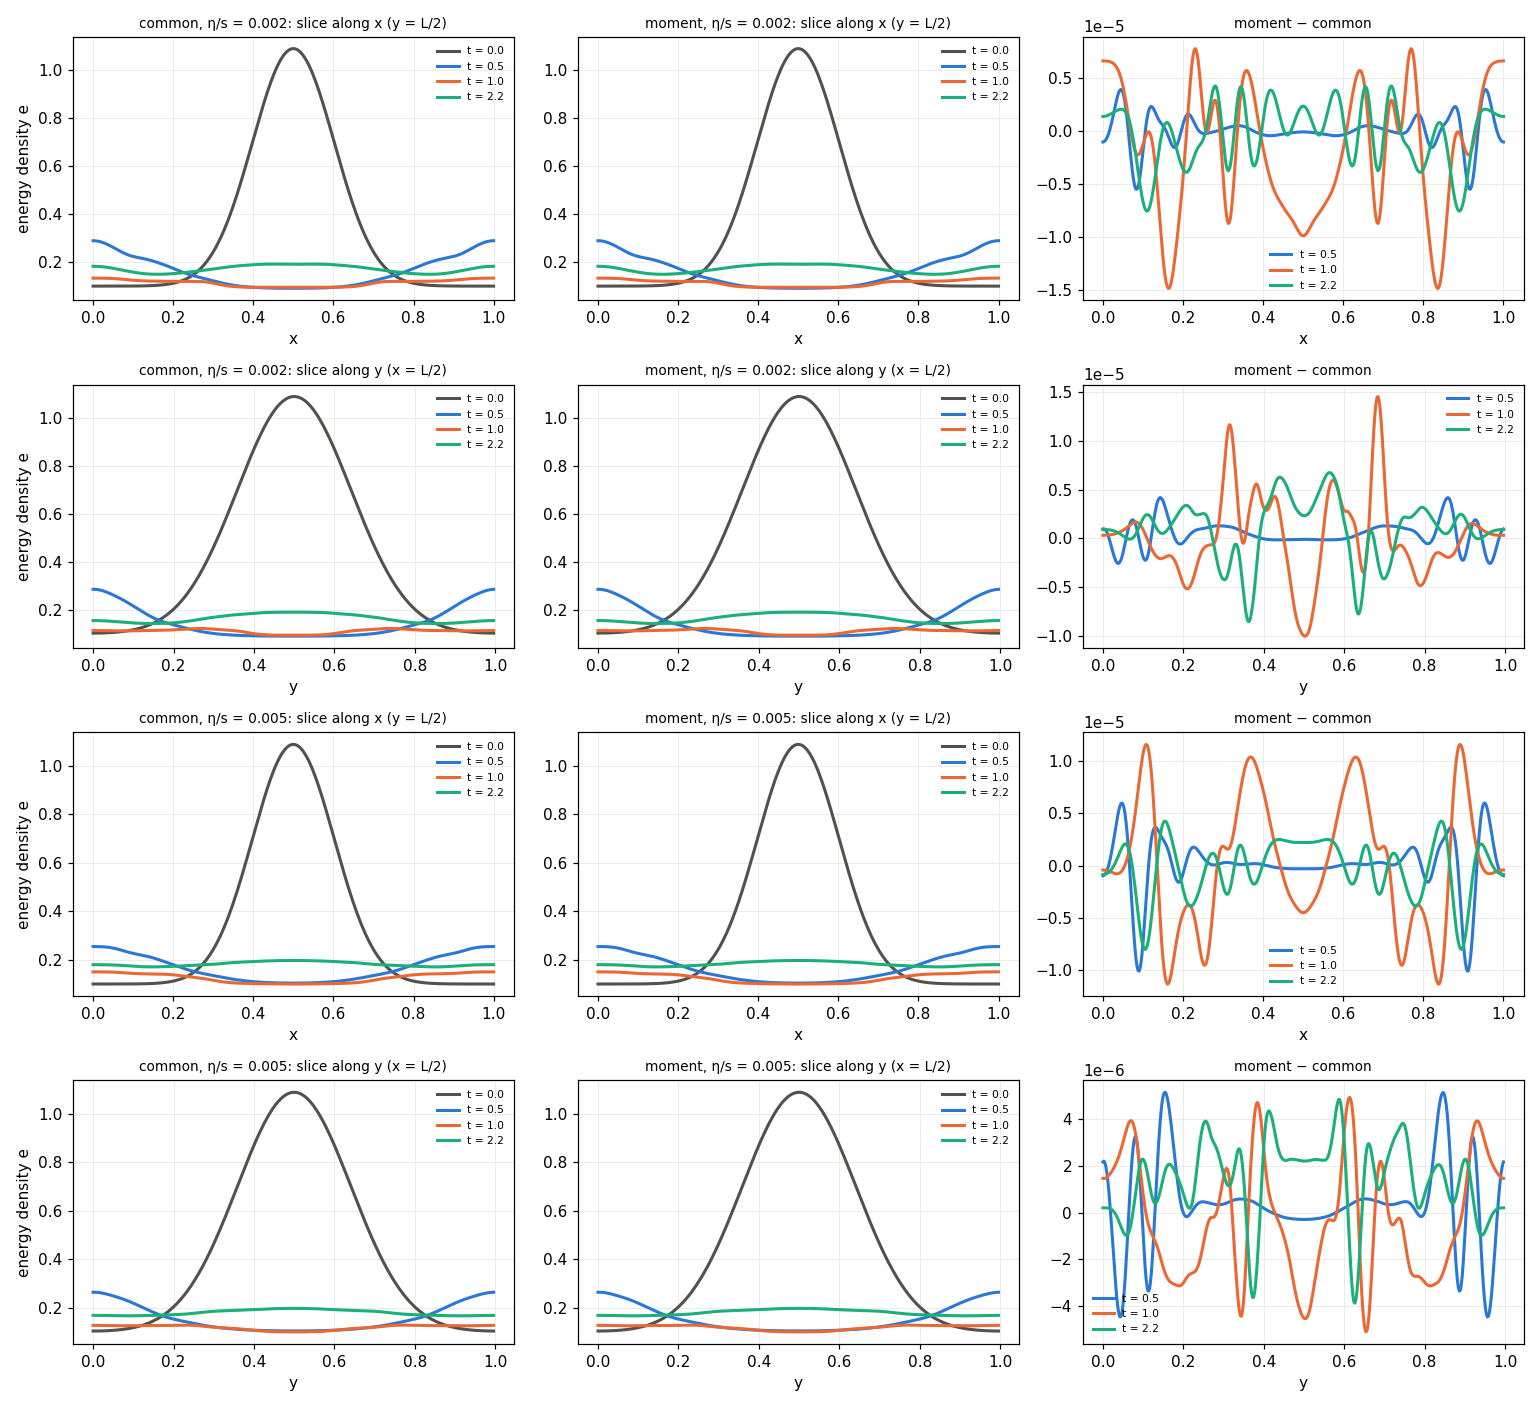
\includegraphics[width=\textwidth]{figs/moment_gaussian.png}
\caption{The Gaussian blob in the full deterministic step: slices of the energy density along $x$ and along $y$ through the centre at
$t=0$, $0.5$, $1$, $2.2$, \texttt{common} (left), \texttt{moment} (middle) and their difference (right, scale $10^{-5}$); two rows per $\eta/s$.}
\label{fig:gauss}
\end{figure}

Nothing is made worse: on the lattice, the jittered lattice and in the nonlinear blob the two schemes agree to $0.2\%$ or better.
The disordered case that matters in practice is the liquid of the stochastic runs; it is tested by the campaign at NERSC.

\begin{figure}[h]
\centering
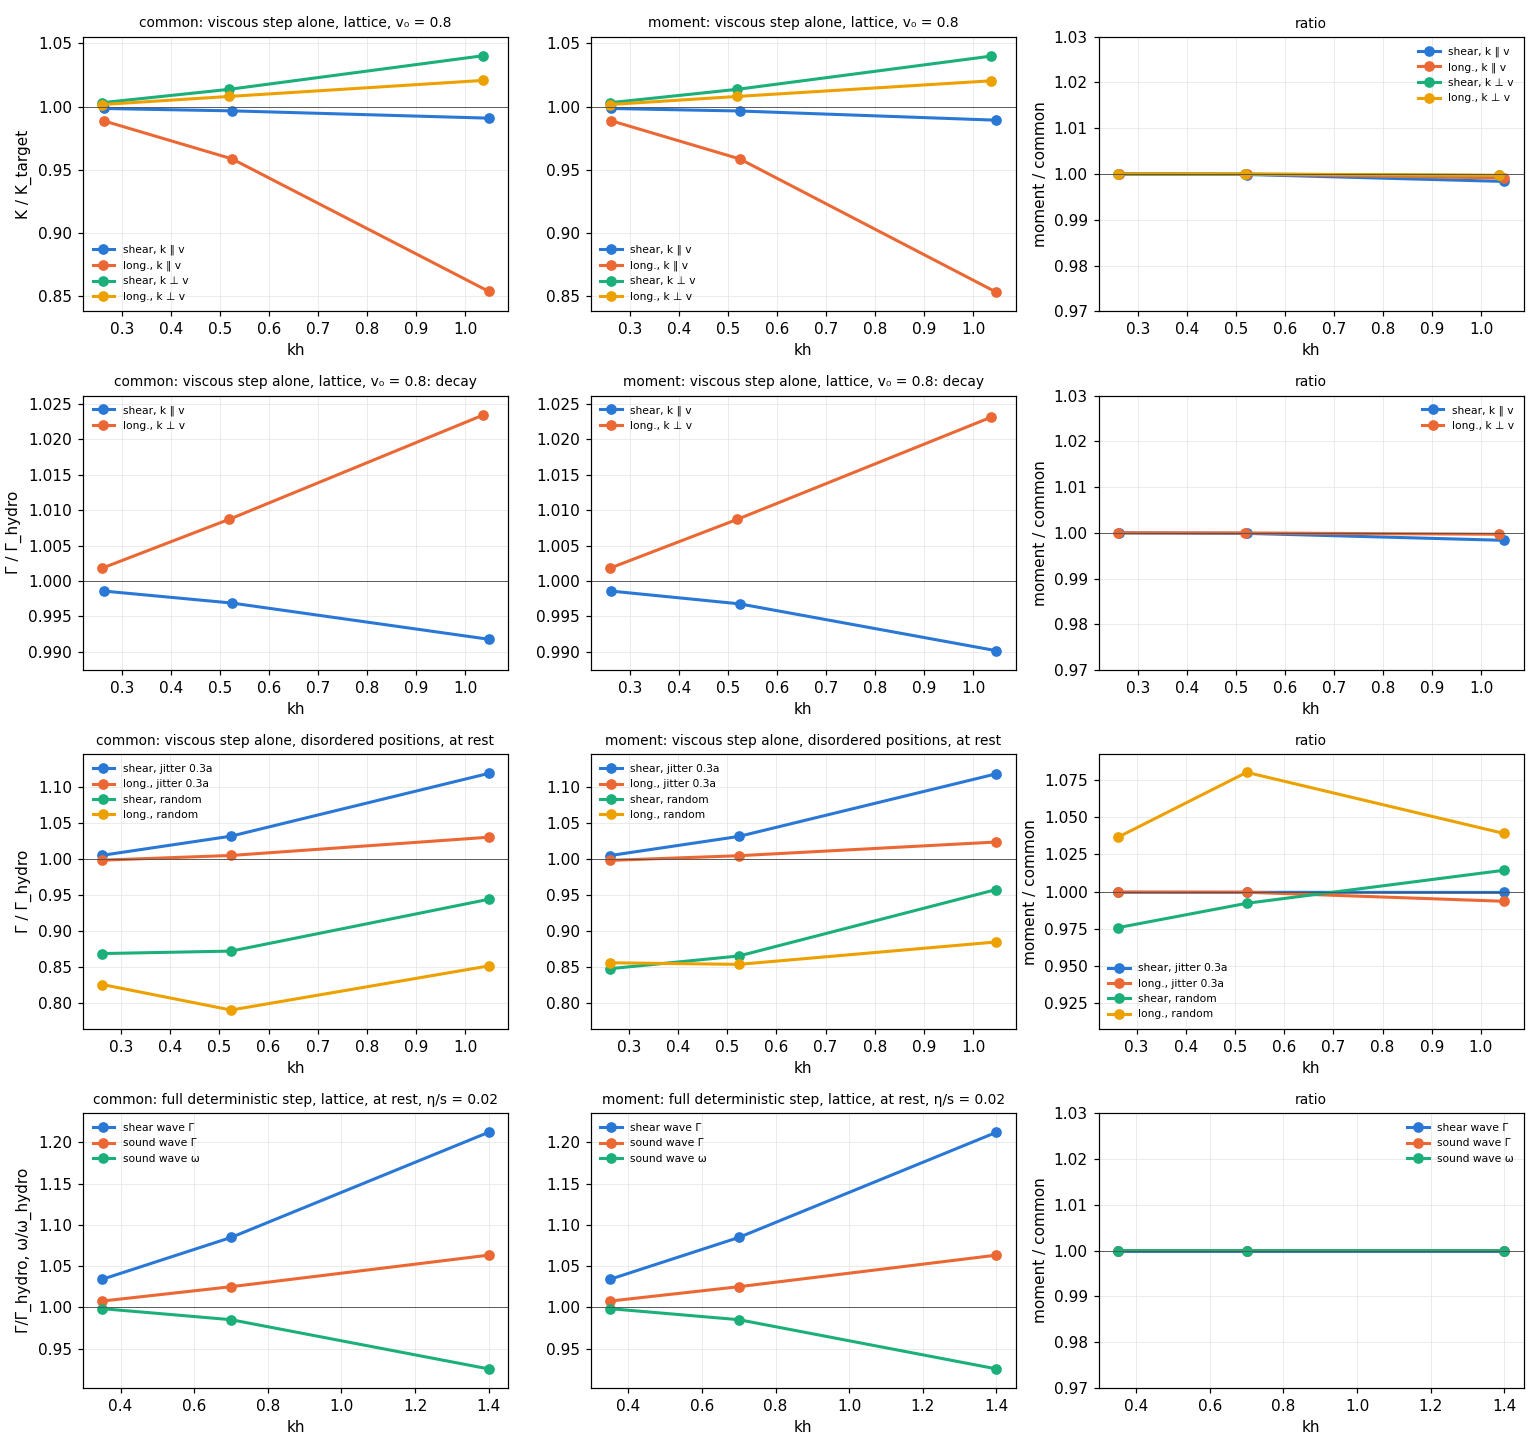
\includegraphics[width=\textwidth]{figs/moment_det.png}
\caption{Deterministic tests, \texttt{common} (left), \texttt{moment} (middle) and their ratio (right).  Rows: $K/K_{\rm target}$ of four modes of the
viscous step alone on the lattice at $v_0=0.8$; the decay rates of its two pure modes; the viscous step alone on disordered positions at rest;
the full deterministic step on the lattice at rest.}
\label{fig:det}
\end{figure}

\section{Stage 1: results from NERSC}
\label{sec:nersc}

Campaign \texttt{moment} (\texttt{nersc/campaign\_moment.txt}, 96 runs, $L=0.6$, $h/a=2$, $s_a=135$, current defaults; each common/moment pair
shares its seeds), packed on 4 debug nodes (job 61359856, 8 min), commit \texttt{d1b5ee6} (before the roundoff fix \texttt{a1b1457}, which
does not affect the comparison).  Analysis: \texttt{examples/boost\_analysis.jl}, groups MOA and MO.

\paragraph{Acceptances and guards.}  Identical to $10^{-3}$: stress $0.960$ / $0.975$, residual $0.711$ / $0.845$ at $v_0=0$ / $0.8$, for both
schemes, alone and in the full step.  No guard fired in any run.

\paragraph{The stochastic step alone} (positions frozen, $t=50$, 8 runs per set).  The kinetic energy of the fluctuations: common $0.989$,
moment $0.988$ at rest; $17.130$, $17.141$ at $v_0=0.8$.  The equal-time $C_{MM}/\chi$ agree within the errors of 8 runs ($\pm0.04$--$0.13$;
\Fig{fig:nersc_moa}).  The shear damping at rest: common $0.79$--$0.98$, moment $0.94$--$1.11$, errors $\pm0.08$--$0.24$ (differences $0.5$--$1.1\sigma$).

\paragraph{The full step} ($t=100$, 16 runs per set; Figs.~\ref{fig:nersc_mo}--\ref{fig:nersc_shear8} and the correlator figures after them, common and moment side by side).
\begin{center}
\begin{tabular}{lcccc}
\hline
 & common, $v_0=0$ & moment, $v_0=0$ & common, $v_0=0.8$ & moment, $v_0=0.8$ \\ \hline
KE$/2VwT$ (predicted $1$; $17.6$) & $0.993$ & $0.992$ & $17.59$ & $17.49$ \\
$\Delta H/H$ at $t=100$ & $-3.5\times10^{-5}$ & $+2.9\times10^{-5}$ & $6.6\times10^{-5}$ & $7.7\times10^{-5}$ \\
shear $\Gamma/\Gamma_{\rm hydro}$, $kh=0.52$, along / across & $1.03(7)$ / $1.03(6)$ & $1.10(3)$ / $1.17(7)$ & $1.49(17)$ / $1.19(8)$ & $0.86(14)$ / $0.98(7)$ \\
shear $\Gamma/\Gamma_{\rm hydro}$, $kh=1.05$, along / across & $1.10(3)$ / $1.02(3)$ & $1.04(5)$ / $1.07(4)$ & $1.10(5)$ / $1.10(4)$ & $1.13(9)$ / $1.00(5)$ \\
\hline
\end{tabular}
\end{center}
The equal-time correlators agree within the errors at every $kh$ (both show $C_{EE}/\chi$ rising to $1.14$--$1.18$ at $kh=1.57$, the
finite-$kh$ correction).  The largest fluctuation is the shear damping along the flow at $v_0=0.8$, $kh=0.52$ (the fundamental mode of the $L=0.6$ box, the
noisiest fit): $1.49(17)$ for common and $0.86(14)$ for moment (\Fig{fig:nersc_fit}; the correlators in \Fig{fig:nersc_shear8} differ only
modestly).  One such $2.9\sigma$ difference among about 16 comparisons is what chance gives; at $kh=1.05$ the two agree.

\paragraph{Deterministic viscous step alone, $v_0=0.8$} (\texttt{examples/moment\_det.jl} set A, rerun as a debug job with the fix below): the
fitted decay rates of common and moment agree to four digits in all twelve cases, with $\Delta S=2\int K\,dt$ to $10^{-4}$ and $\Delta H/H\sim10^{-13}$.
For a momentum perturbation along the flow (longitudinal with $\bm k\parallel\bm v$, shear with $\bm k\perp\bm v$) the entropy deficit at fixed lab
energy, $D=\sum_a[S_a(e_a,\bar{\bm m})-S_a(e_a,\bm m_a)]$, is negative: $K/D$ is then not a rate, and in the scripts it made the run length
negative, so these cases had never run (they appeared as zeros).  With $|K/D|$ setting the run length they run, are stable, and decay at
$0.35$--$1.27\,|K/D|$ --- not a single exponential at that rate; only the two pure modes give clean rates, as the laptop results above already use.

\paragraph{More runs at $v_0=0.8$} (campaign \texttt{moment\_a}, job 61361957, 4 debug nodes, 8 min; $L=0.6$, 64 runs per scheme, new seeds;
Figs.~\ref{fig:nersc_A_fit}--\ref{fig:nersc_A_shear}):
\begin{center}
\begin{tabular}{lcc}
\hline
$v_0=0.8$, $L=0.6$, 64 runs & common & moment \\ \hline
shear $\Gamma/\Gamma_{\rm hydro}$, $kh=0.52$, along / across & $1.26(9)$ / $1.20(6)$ & $1.12(10)$ / $1.13(5)$ \\
shear $\Gamma/\Gamma_{\rm hydro}$, $kh=1.05$, along / across & $1.20(5)$ / $1.09(3)$ & $1.19(5)$ / $1.10(3)$ \\
KE$/2VwT$ (predicted $17.6$) & $17.50$ & $17.47$ \\
\hline
\end{tabular}
\end{center}
The difference along the flow at $kh=0.52$ is now $1.0\sigma$ ($2.9\sigma$ with 16 runs): a fluctuation.  The equal-time correlators agree at
every $kh$.

\paragraph{A larger box} (campaign \texttt{moment\_b}, job 61361958, 4 regular nodes, 42 min; $L=1.2$, $N=2688$, 32 runs per set, $kh=0.26$, $0.52$,
$0.79$; Figs.~\ref{fig:nersc_B_equaltime}--\ref{fig:nersc_B_shearperp}):
\begin{center}
\begin{tabular}{lcc}
\hline
$L=1.2$, 32 runs & common & moment \\ \hline
KE$/2VwT$, $v_0=0$ / $0.8$ (predicted $1$ / $17.6$) & $0.994$ / $17.54$ & $0.994$ / $17.50$ \\
shear $\Gamma/\Gamma_{\rm hydro}$ at rest, $kh=0.26$, along / across & $0.94(12)$ / $1.10(9)$ & $0.95(12)$ / $0.84(11)$ \\
shear $\Gamma/\Gamma_{\rm hydro}$ at rest, $kh=0.52$, along / across & $1.14(5)$ / $1.07(6)$ & $1.15(6)$ / $1.09(4)$ \\
shear $\Gamma/\Gamma_{\rm hydro}$, $v_0=0.8$, $kh=0.26$, along / across & $1.01(21)$ / $1.09(17)$ & $1.53(34)$ / $1.01(15)$ \\
shear $\Gamma/\Gamma_{\rm hydro}$, $v_0=0.8$, $kh=0.52$, along / across & $1.28(13)$ / $1.11(6)$ & $1.25(14)$ / $1.05(7)$ \\
\hline
\end{tabular}
\end{center}
The two schemes agree within the errors at every wavevector, at rest and at $v_0=0.8$, and so do the equal-time correlators (the largest
difference, $1.3\sigma$, is along the flow at $kh=0.26$, the noisiest fit).

\paragraph{Verdict.}  No difference between common and moment beyond the statistics: acceptances, guards, kinetic energy, equal-time
correlators, shear and sound at rest and at $v_0=0.8$, along and across the flow, in the boxes $L=0.6$ (16 and 64 runs) and $1.2$ (32 runs), the
stochastic step alone and the deterministic viscous step.
The default stays \texttt{common} until the owner decides.

\begin{figure}[p]
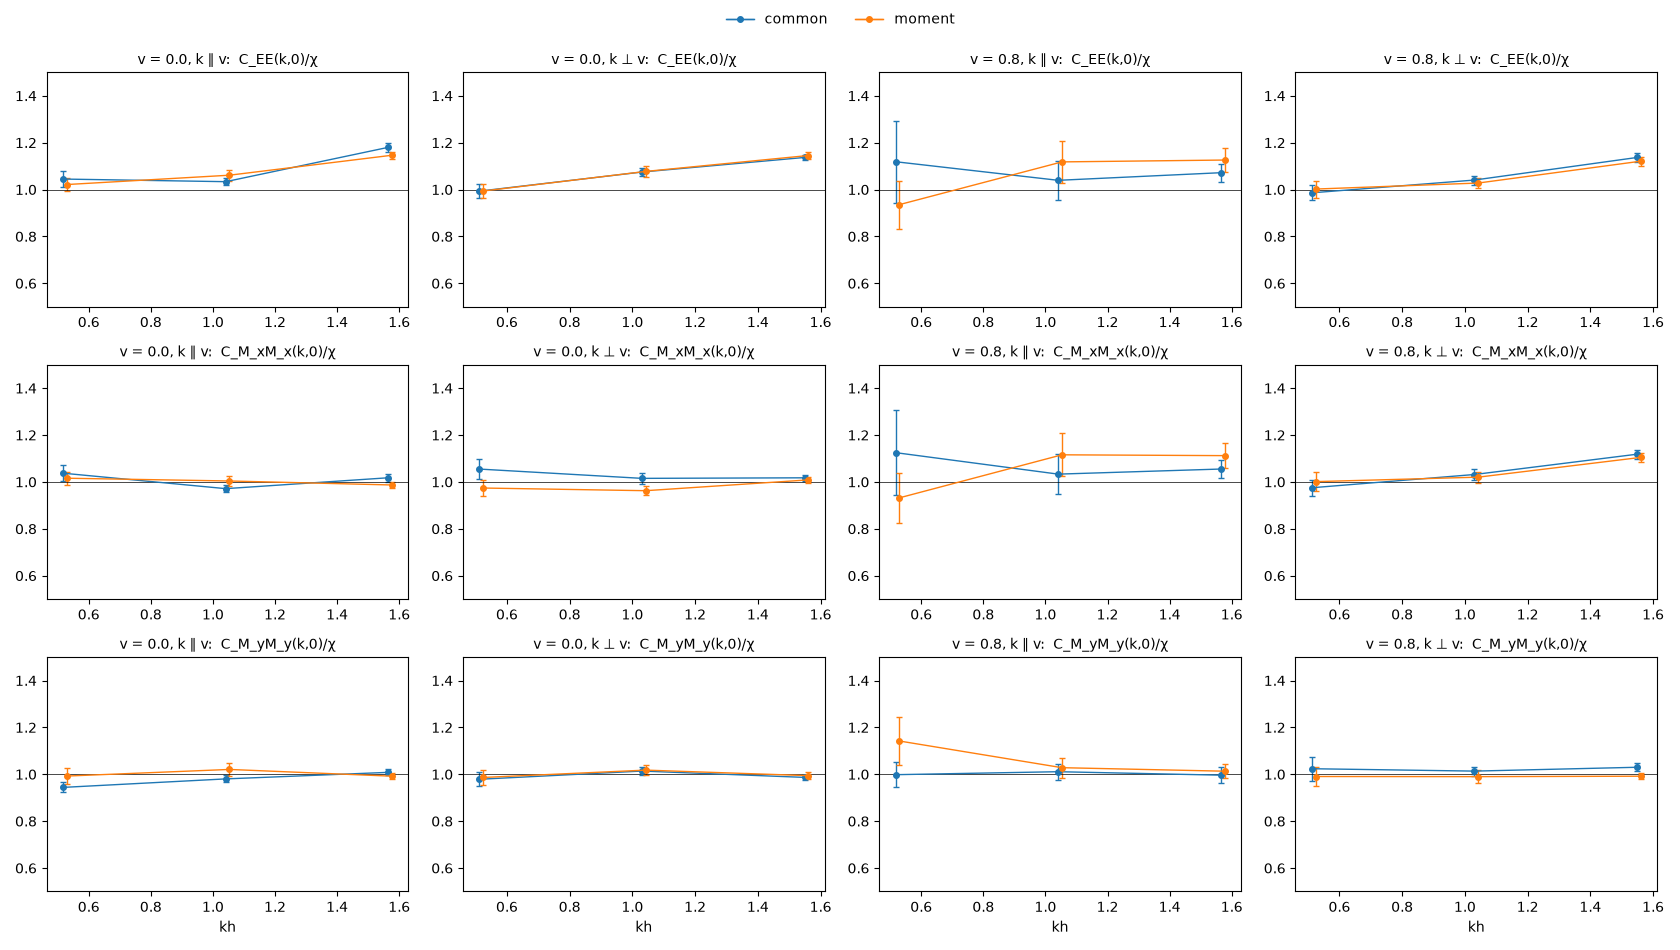
\includegraphics[width=\textwidth]{figs/moment_nersc_equaltime_MO.png}
\caption{Campaign \texttt{moment}, the full step: equal-time $C_{AA}(\bm k,0)/\chi_{AA}$ for $A=E$, $M_x$, $M_y$ (rows), at $v_0=0$ and $0.8$ with $\bm k$ along and across $x$ (columns); common and moment overlaid (key at the top), 16 runs each, jackknife errors.}
\label{fig:nersc_mo}
\end{figure}
\begin{figure}[p]
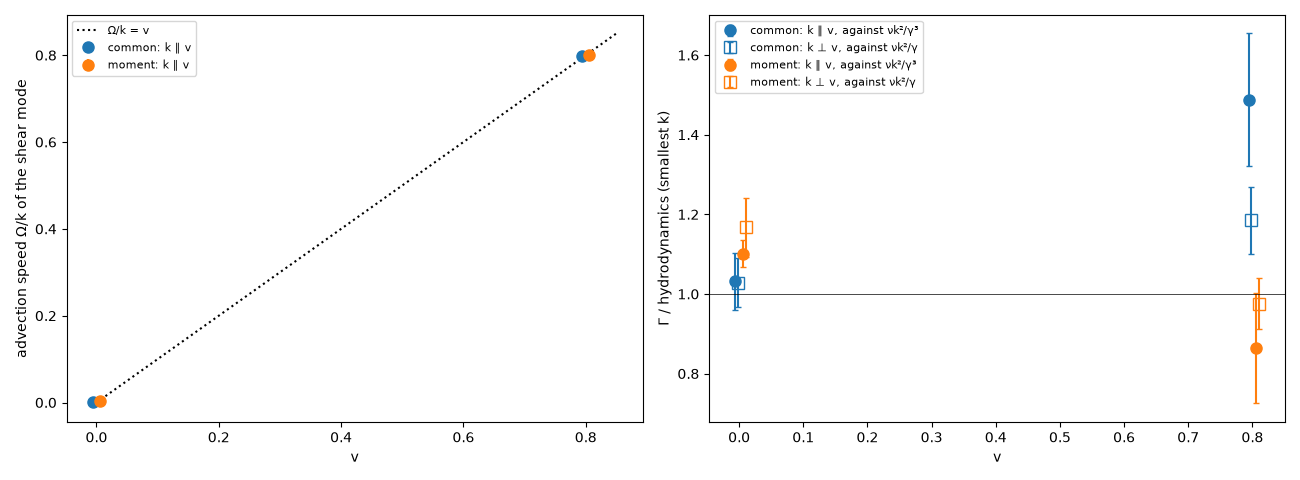
\includegraphics[width=\textwidth]{figs/moment_nersc_fit_MO.png}
\caption{The full step: the fitted advection speed $\Omega/k$ (left) and damping $\Gamma/\Gamma_{\rm hydro}$ (right) of the shear mode at $kh=0.52$ against $v_0$; common blue, moment orange; filled $\bm k\parallel\bm v$ (against $\nu k^2/\gamma^3$), open $\bm k\perp\bm v$ (against $\nu k^2/\gamma$).}
\label{fig:nersc_fit}
\end{figure}
\begin{figure}[p]
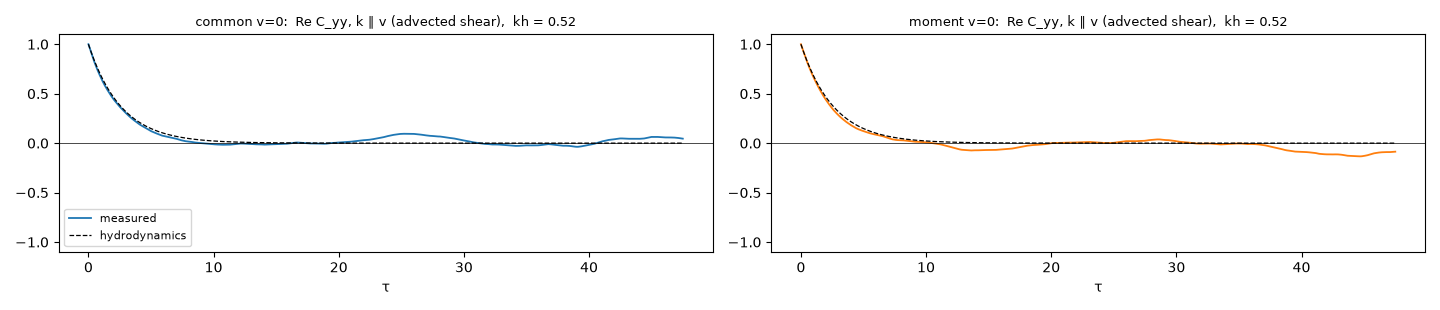
\includegraphics[width=\textwidth]{figs/moment_nersc_shear_v0.0_MO.png}
\caption{The full step at rest: the shear mode $\mathrm{Re}\,C_{yy}(k\hat x,\tau)$ at $kh=0.52$, common (left) and moment (right); dashed hydrodynamics.}
\label{fig:nersc_shear0}
\end{figure}
\begin{figure}[p]
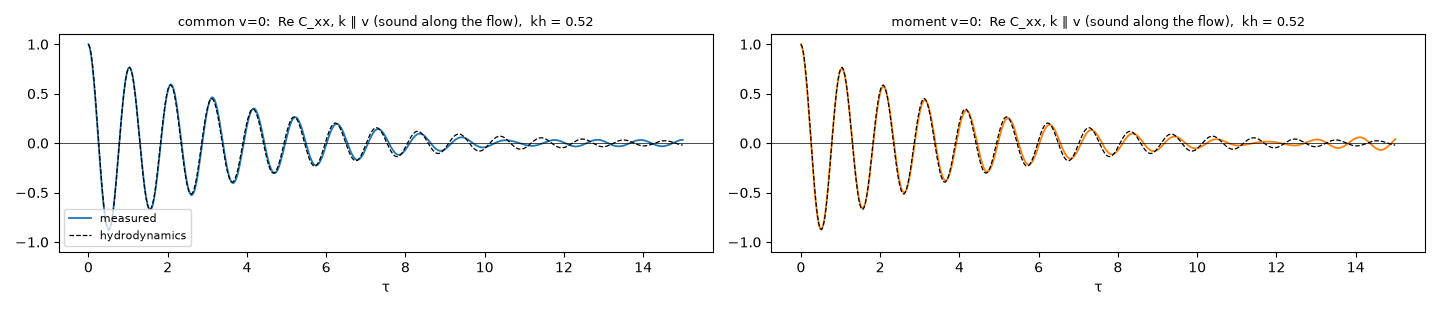
\includegraphics[width=\textwidth]{figs/moment_nersc_soundpar_v0.0_MO.png}
\caption{The full step at rest: sound, $\mathrm{Re}\,C_{xx}(k\hat x,\tau)$ at $kh=0.52$, common (left) and moment (right); dashed hydrodynamics.}
\end{figure}
\begin{figure}[p]
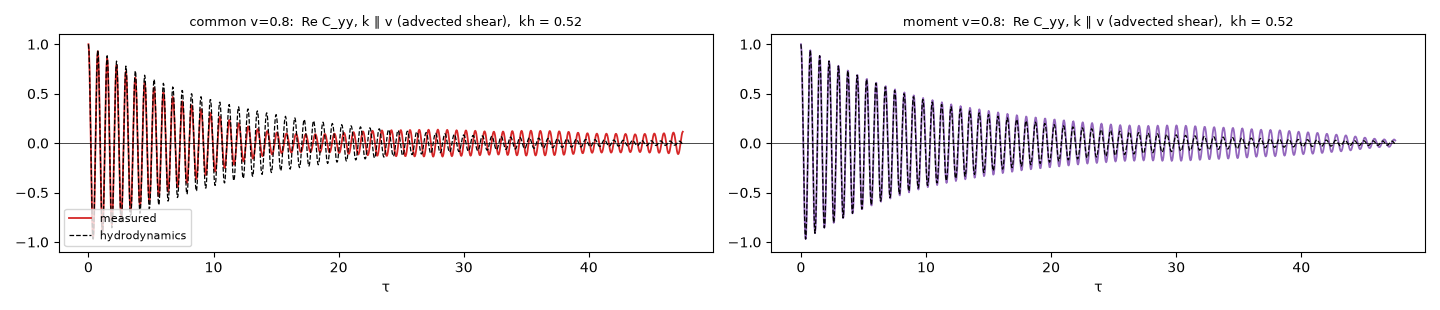
\includegraphics[width=\textwidth]{figs/moment_nersc_shear_v0.8_MO.png}
\caption{The full step at $v_0=0.8$: the advected shear mode $\mathrm{Re}\,C_{yy}(k\hat x,\tau)$ at $kh=0.52$, common (left) and moment (right); dashed hydrodynamics.  The fits give $\Gamma/\Gamma_{\rm hydro}=1.49(17)$ and $0.86(14)$.}
\label{fig:nersc_shear8}
\end{figure}
\begin{figure}[p]
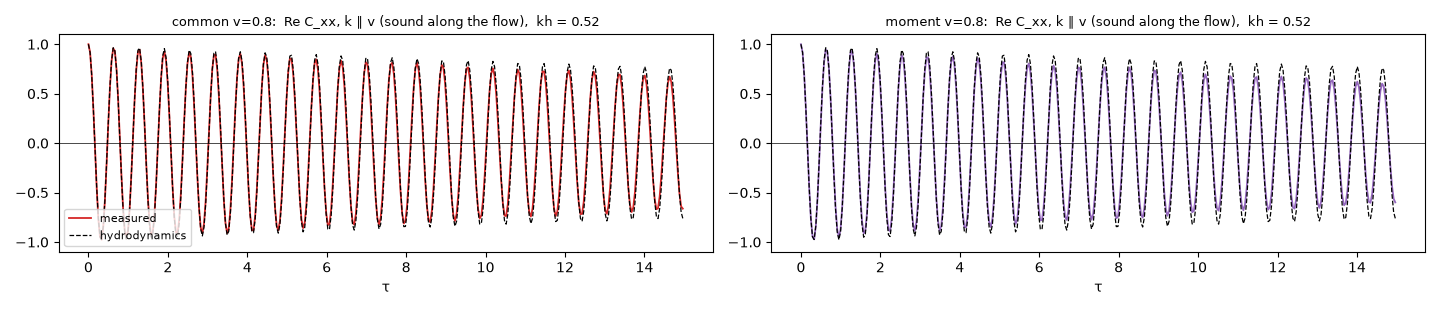
\includegraphics[width=\textwidth]{figs/moment_nersc_soundpar_v0.8_MO.png}
\caption{The full step at $v_0=0.8$: sound along the flow, $\mathrm{Re}\,C_{xx}(k\hat x,\tau)$, common (left) and moment (right).}
\end{figure}
\begin{figure}[p]
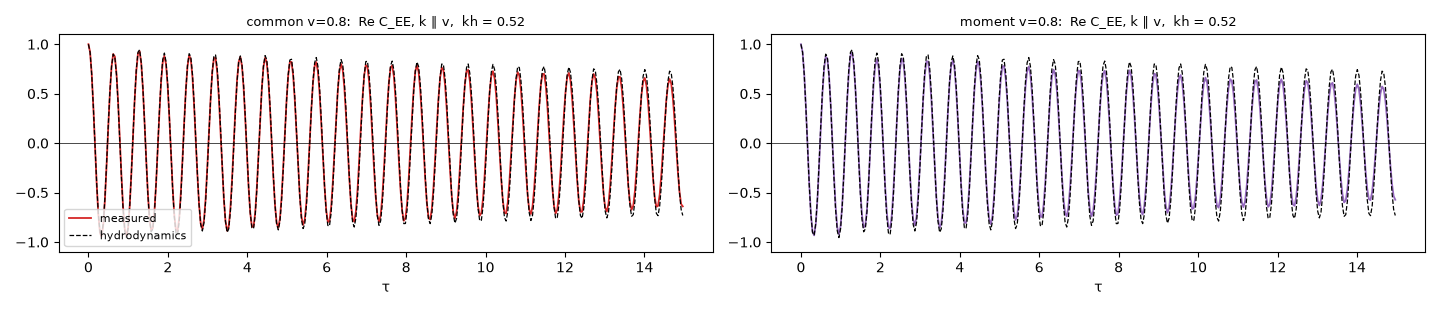
\includegraphics[width=\textwidth]{figs/moment_nersc_EEpar_v0.8_MO.png}
\caption{The full step at $v_0=0.8$: $\mathrm{Re}\,C_{EE}(k\hat x,\tau)$, common (left) and moment (right).}
\end{figure}
\begin{figure}[p]
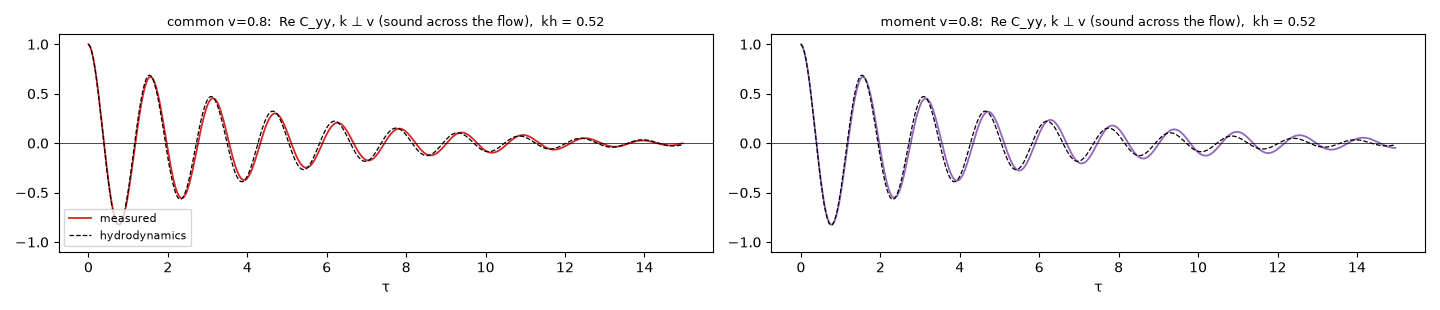
\includegraphics[width=\textwidth]{figs/moment_nersc_soundperp_v0.8_MO.png}
\caption{The full step at $v_0=0.8$: sound across the flow, $\mathrm{Re}\,C_{yy}(k\hat y,\tau)$, common (left) and moment (right).}
\end{figure}
\begin{figure}[p]
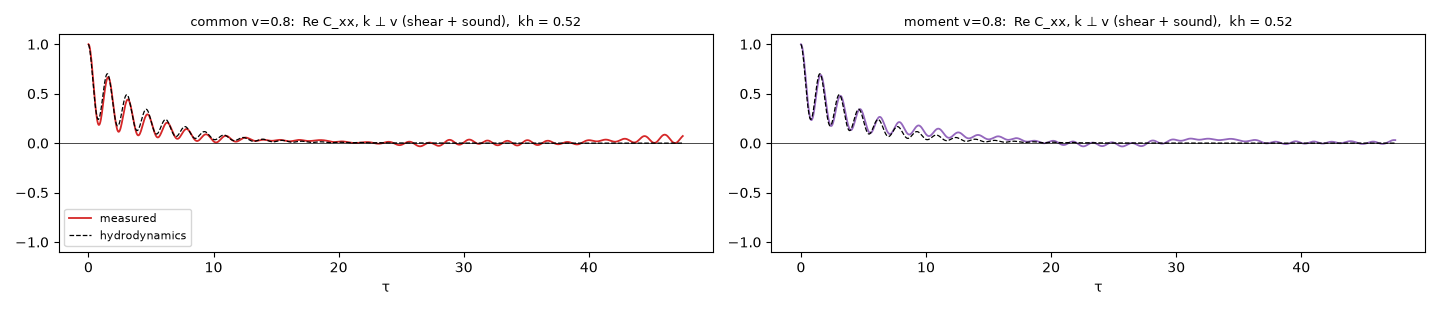
\includegraphics[width=\textwidth]{figs/moment_nersc_shearperp_v0.8_MO.png}
\caption{The full step at $v_0=0.8$: across the flow, $\mathrm{Re}\,C_{xx}(k\hat y,\tau)$ (shear and sound), common (left) and moment (right).}
\end{figure}
\begin{figure}[p]
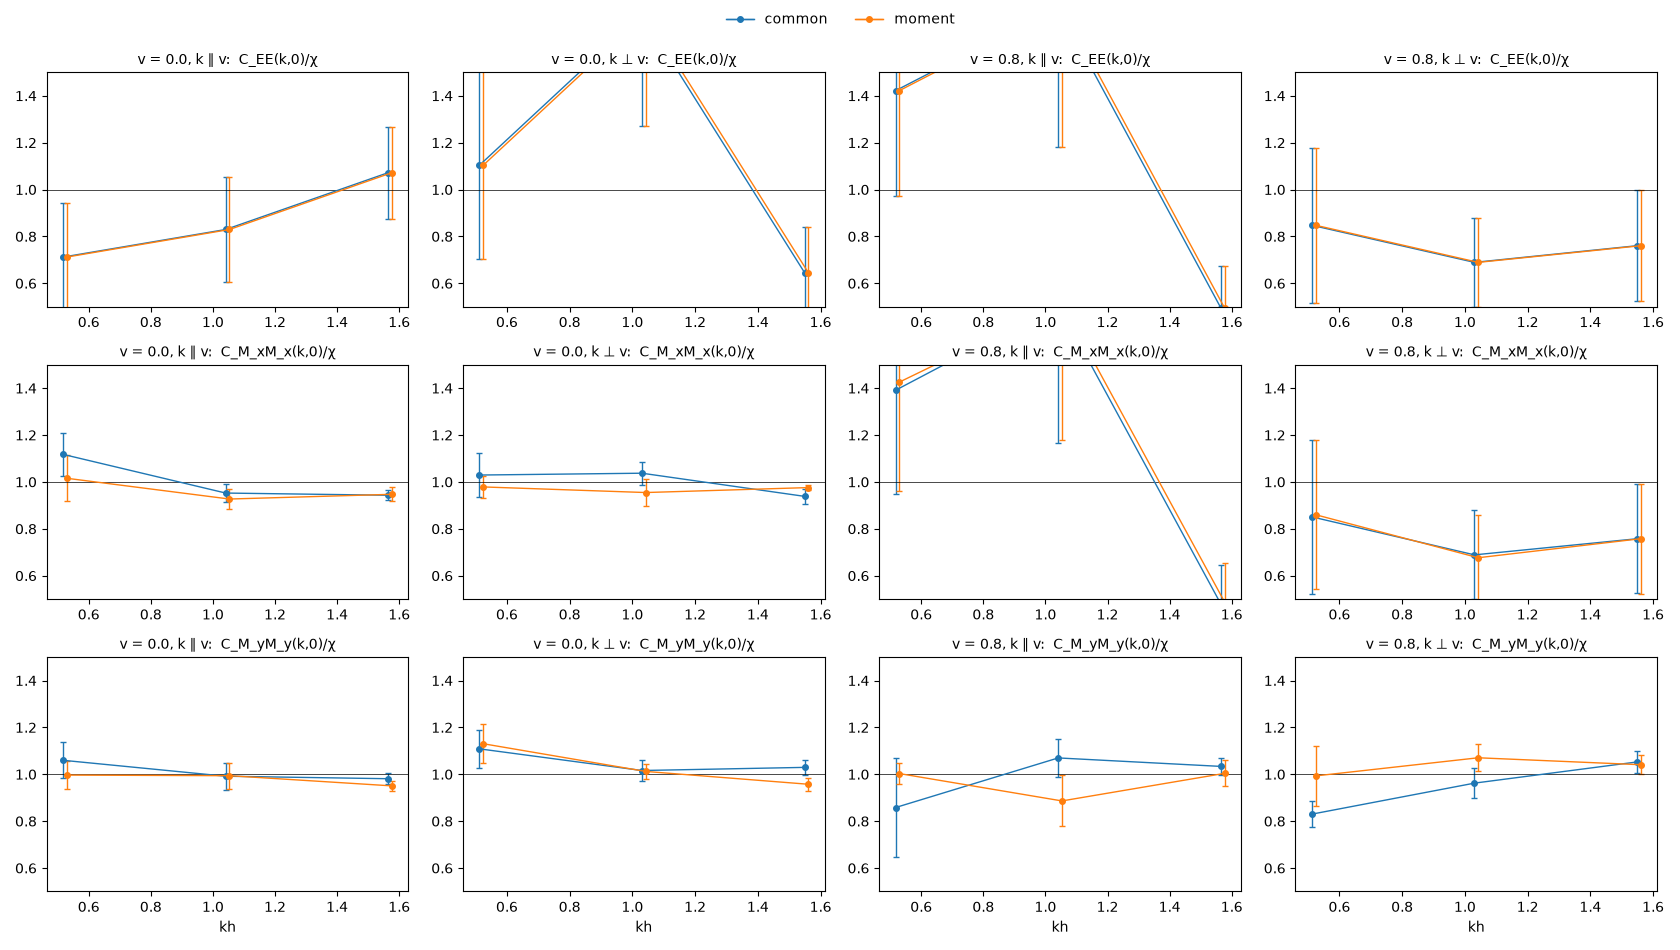
\includegraphics[width=\textwidth]{figs/moment_nersc_equaltime_MOA.png}
\caption{Campaign \texttt{moment}, the stochastic step alone (positions frozen): equal-time $C_{AA}(\bm k,0)/\chi_{AA}$, common and moment, 8 runs each.  $E$ does not change in this step, so its rows show the initial state, the same for both.}
\label{fig:nersc_moa}
\end{figure}
\begin{figure}[p]
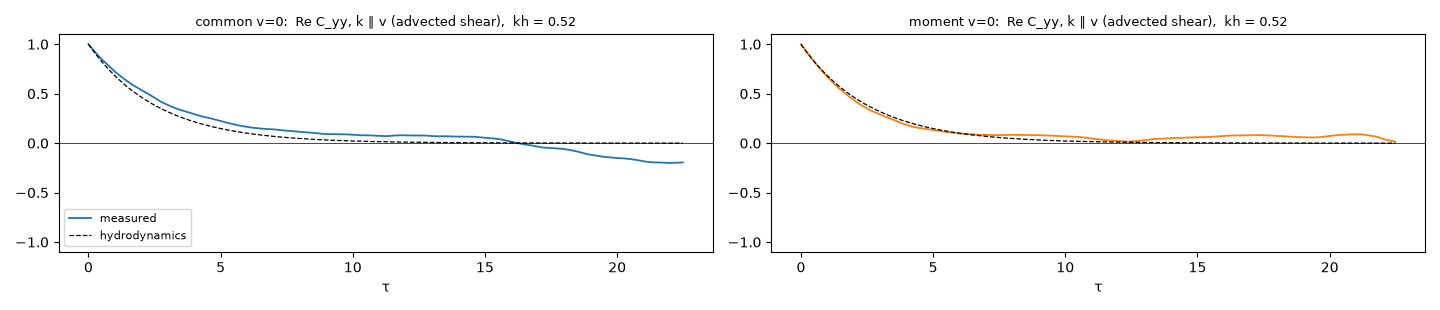
\includegraphics[width=\textwidth]{figs/moment_nersc_shear_v0.0_MOA.png}
\caption{The stochastic step alone at rest: the shear mode $\mathrm{Re}\,C_{yy}(k\hat x,\tau)$ at $kh=0.52$, common (left) and moment (right).  (At $v_0=0.8$ there is no advection without the ideal step, so the moving correlators of this set are not shown.)}
\end{figure}

\section{Stage 2: results on the laptop}
\label{sec:laptop2}

\paragraph{The ratios} (\texttt{test/testhastings.jl}; jittered lattice moving with $v_0=0.5$, thermal momenta at $s_a\approx16$, twice the usual time
step).  The coefficients computed from the state of a particle equal those of \texttt{build\_stars} to $4\times10^{-12}$.  \Eq{qstress2} equals the
ratio of the two Gaussian densities of $\xi$ to $4\times10^{-15}$; \Eq{qresid} equals the ratio of the densities of the conditioned draws on the
zero-virial subspace of the $2n\approx110$ bond components to $6\times10^{-8}$ (the roundoff of the direct side).  The residual ratios range over
$-86\le\ln(q'/q)\le0.3$ in these stars: large, see below.

\paragraph{The equilibrium} (\texttt{examples/hastings\_baseline.jl}, \texttt{moment}, \texttt{SPH\_MEASURE=einstein}, coefficients rebuilt, eight runs of $200$
viscous time steps).  the ratios $\langle\delta m_x^2\rangle/C_{xx}$ and $\langle\delta m_y^2\rangle/C_{yy}$ (columns $x$, $y$) and the residual acceptance, without and
with the correction:
\begin{center}
\begin{tabular}{lcccc}
\hline
 & \multicolumn{2}{c}{without} & \multicolumn{2}{c}{with the correction} \\
$s_a$, $v_0$, $\Delta t/\Delta t_{\rm visc}$ & $x$, $y$ & acc. & $x$, $y$ & acc. \\ \hline
$16$, $0$, $\frac12$   & $1.086$, $1.083$ & $0.60$ & $0.996$, $0.994$ & $0.41$ \\
$16$, $0$, $\frac18$   & $1.146$, $1.140$ & $0.79$ & $1.003$, $0.996$ & $0.66$ \\
$16$, $0.8$, $\frac12$ & $1.023$, $1.067$ & $0.65$ & $1.007$, $0.998$ & $0.22$ \\
$16$, $0.8$, $\frac18$ & $0.961$, $1.088$ & $0.83$ & $1.003$, $0.998$ & $0.45$ \\
$54$, $0$, $\frac12$   & $1.033$, $1.031$ & $0.68$ & $1.007$, $1.003$ & $0.65$ \\
$54$, $0$, $\frac18$   & $1.056$, $1.050$ & $0.83$ & $1.001$, $0.997$ & $0.82$ \\
$54$, $0.8$, $\frac12$ & $0.995$, $1.021$ & $0.75$ & $1.005$, $0.991$ & $0.47$ \\
$54$, $0.8$, $\frac18$ & $0.973$, $1.033$ & $0.87$ & $0.999$, $1.001$ & $0.70$ \\
\hline
\end{tabular}
\end{center}
The errors are $\pm0.002$ to $\pm0.007$.  With the correction every value is $1$ within the errors (the largest deviation $1.007\pm0.0025$), and
$\langle\ln T_a\rangle$ is exact; the bias of up to $15\%$ is gone.  The stress acceptance is unchanged ($0.94$--$0.98$), and the wall time grows by
about $20\%$.

\paragraph{With the Liouville measure} (the default; the exact target is then $e^{S_a-\ln T_a+\bm\mu\cdot\delta\bm m}$ per particle, with the vote entropy of the
step; 16 runs per case).  The ratios $\langle\delta m_x^2\rangle/C_{xx}$, $\langle\delta m_y^2\rangle/C_{yy}$ and $\langle\ln T_a\rangle$ minus its exact value:
\begin{center}
\begin{tabular}{lccc}
\hline
$s_a$, $v_0$, $\Delta t/\Delta t_{\rm visc}$ & without: $x$, $y$ & with: $x$, $y$ & with: $\langle\ln T_a\rangle-$ exact \\ \hline
$16$, $0$, $\frac12$   & $1.107$, $1.104$ & $1.004$, $0.999$ & $-0.0001(3)$ \\
$16$, $0$, $\frac18$   & $1.169$, $1.165$ & $1.000$, $1.000$ & $+0.0002(1)$ \\
$16$, $0.8$, $\frac12$ & $1.019$, $1.075$ & $1.002$, $0.994$ & $+0.0003(6)$ \\
$16$, $0.8$, $\frac18$ & $0.955$, $1.102$ & $0.999$, $0.995$ & $+0.0004(4)$ \\
$54$, $0$, $\frac12$   & $1.041$, $1.036$ & $1.001$, $0.995$ & $+0.0001(1)$ \\
$54$, $0$, $\frac18$   & $1.058$, $1.056$ & $1.002$, $1.001$ & $+0.0000(1)$ \\
$54$, $0.8$, $\frac12$ & $0.992$, $1.026$ & $0.999$, $0.999$ & $+0.0002(1)$ \\
$54$, $0.8$, $\frac18$ & $0.972$, $1.031$ & $1.001$, $0.996$ & $+0.0002(1)$ \\
\hline
\end{tabular}
\end{center}
The errors of the ratios are $\pm0.002$ to $\pm0.005$; every value with the correction is within $2\sigma$ of $1$.  Without it the bias is somewhat
larger than with the Einstein measure (up to $17\%$).  The acceptances are as before.  (The exact draw of the start rejects the rare states
beyond the light cone, toward which the Liouville weight grows.)

\paragraph{What is recorded.}  \texttt{SPH\_HASTINGS} is a setting, so every run record says whether the correction was on.  With it,
\texttt{stochastic\_step!} returns the mean and rms of $\ln(q'/q)$ over the proposals of each sweep, and \texttt{examples/equilibrium.jl} records them
per record window, next to the acceptances, as \texttt{hast\_lq\_\{stress,resid\}\_\{mean,rms\}}; without the correction nothing is written.  In a short run
at $s_a=541$, $v_0=0$ the residual log ratios have an rms of $0.04$ and the stress log ratios are below $10^{-3}$.

\paragraph{A cap on the Lorentz factor} (\texttt{SPH\_GAMMA\_MAX}, default $100$, since 2026-11-15).  At $s_a=16$ without the correction a particle
reached $1-v^2\approx10^{-16}$ ($\gamma\approx10^8$) and the comoving structures failed (\Sect{sec:nersc2}).  Near the light cone the inversion of the
equation of state loses accuracy as $10^{-16}\gamma^2$ (relative error of $1-v^2$, $T$, $S$: $7\times10^{-12}$ at $\gamma=100$, $4\times10^{-8}$ at $10^4$,
$5\times10^{-4}$ at $10^6$).  A state with
\st
\gamma>\gamma_{\max}=100,\qquad |\bm v|^2>1-\gamma_{\max}^{-2}=1-10^{-4},
\stp
now has no weight in the votes, the equilibrium start and hybrid Monte Carlo (all through the particle entropy), and the comoving
structures are built with the velocity capped there.  Bit-identical for every run below the cap.  At $s_a=16$ at rest the uncorrected run
now completes ($11\%$ of the residual proposals are rejected at the cap).  The large residual log ratios remain there (median rms per
window $2.6\times10^3$): particles at $\gamma\sim10$--$100$, where one move changes $\det\ell_a=\gamma^{-2}$ and $f_{ab}$ by large factors, are common at
$s_a=16$ ($|\bm v|>0.99$ in $0.1\%$ of the samples).  The correction is still exact there, but the residual move is then decided by $q'/q$.
$s_a\approx16$ is the edge of the method.

\paragraph{The price: the residual acceptance.}  It falls, most at low entropy per particle in a moving fluid ($0.65\to0.22$ at $s_a=16$, $v_0=0.8$,
$\Delta t=\frac12\Delta t_{\rm visc}$).  The residual proposal lives in about $2n\approx110$ dimensions, and its density changes with the coefficients of
particle $a$: the normalization in \Eq{qresid} moves by about $n$ times the relative change $\epsilon$ of the coefficients in one move, and the
quadratic form compensates it only on average, so
\st
\ln\frac{q'}{q}\sim\sqrt{2n}\;\epsilon .
\stp
The relative change $\epsilon$ is largest when the coefficients depend strongly on $\bm m_a$ (a moving fluid, through $\ell_a$, $f_{ab}$ and $\gamma_a$) and
when a move changes $\bm m_a$ much (low $s_a$, large $\Delta t$).  The acceptance recovers at smaller $\Delta t$ ($0.45$ at $\frac18$).  Rejections slow the
damping of the residual modes; they do not bias the equilibrium.  Whether the lower acceptance matters for the dynamics, i.e.\ for the
damping of the lattice modes and the correlators, is for the runs at NERSC.
=======
\begin{figure}[p]
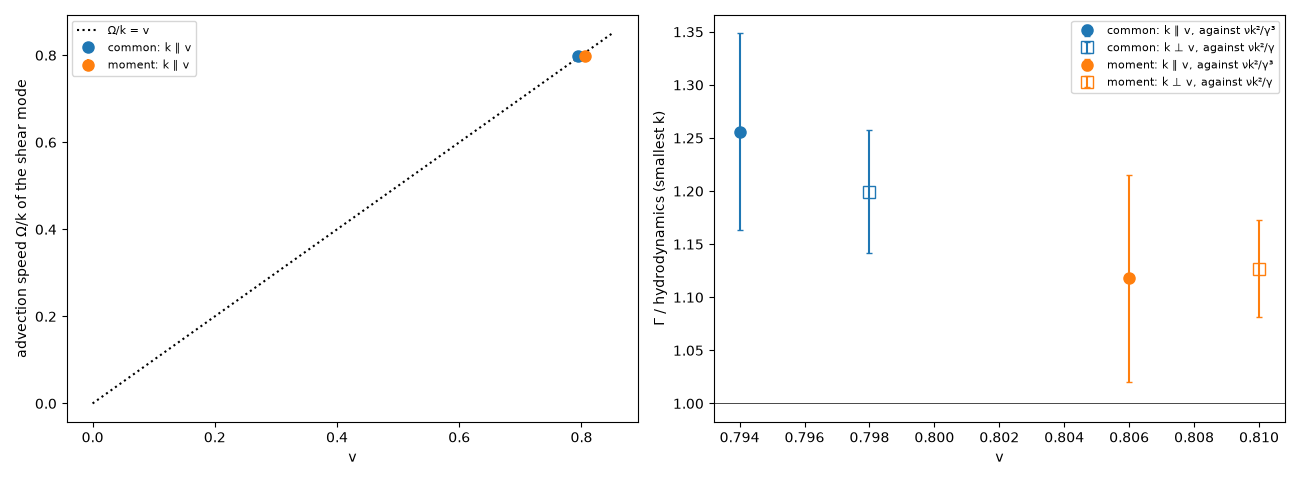
\includegraphics[width=\textwidth]{figs/moment_nersc_A_fit.png}
\caption{Campaign \texttt{moment\_a} ($v_0=0.8$, $L=0.6$, 64 runs per scheme): $\Omega/k$ and $\Gamma/\Gamma_{\rm hydro}$ of the shear mode at $kh=0.52$; common blue,
moment orange; filled along, open across the flow.}
\label{fig:nersc_A_fit}
\end{figure}
\begin{figure}[p]
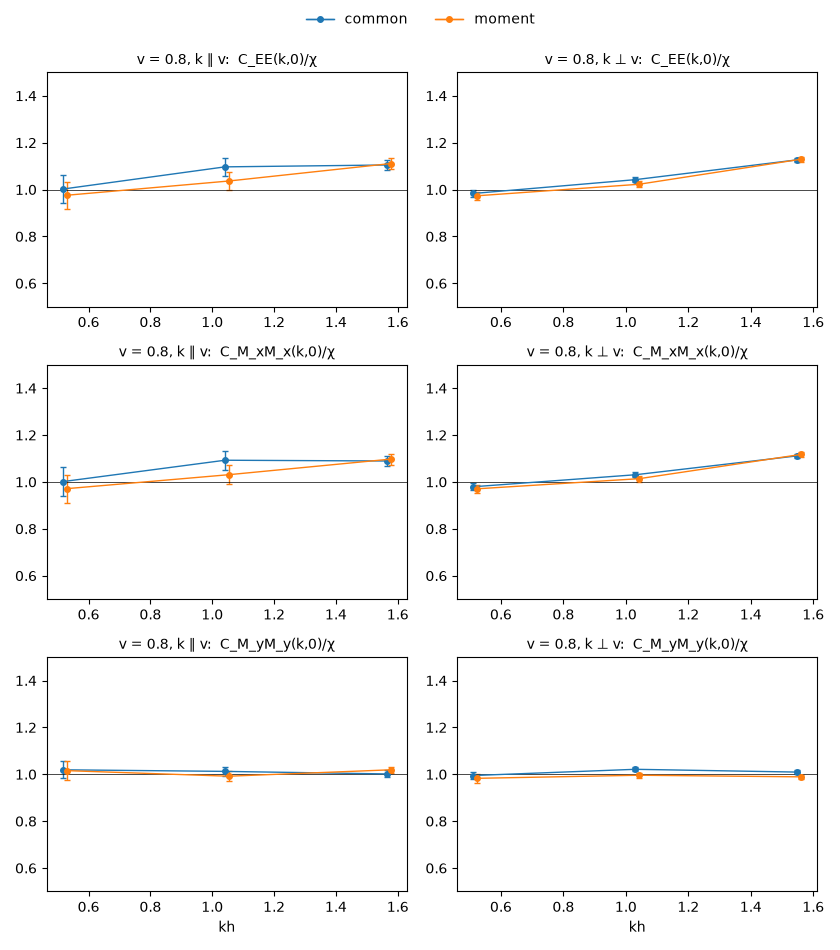
\includegraphics[width=\textwidth]{figs/moment_nersc_A_equaltime.png}
\caption{Campaign \texttt{moment\_a}: equal-time $C_{AA}(\bm k,0)/\chi_{AA}$ at $v_0=0.8$, common and moment, 64 runs each.}
\end{figure}
\begin{figure}[p]
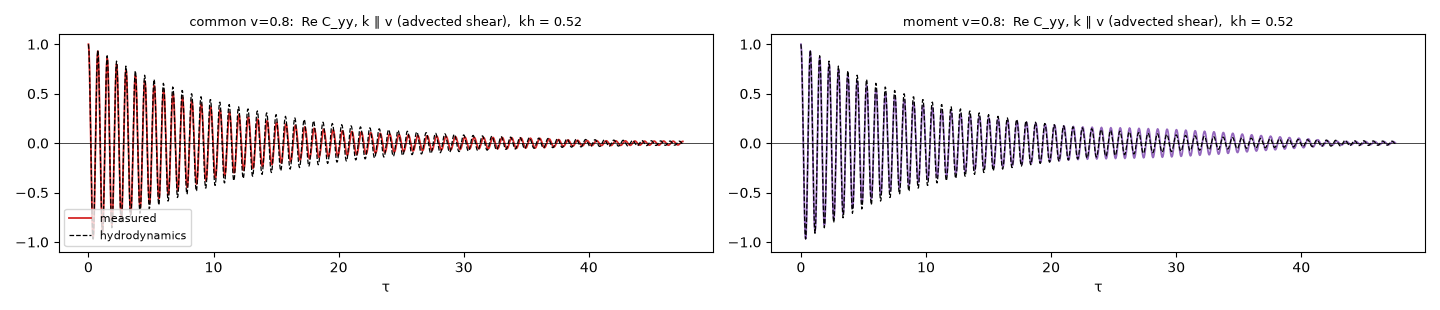
\includegraphics[width=\textwidth]{figs/moment_nersc_A_shear_v0.8.png}
\caption{Campaign \texttt{moment\_a}: the advected shear mode $\mathrm{Re}\,C_{yy}(k\hat x,\tau)$ at $kh=0.52$, common (left) and moment (right), 64 runs each.}
\label{fig:nersc_A_shear}
\end{figure}

%======================================================================
\begin{figure}[p]
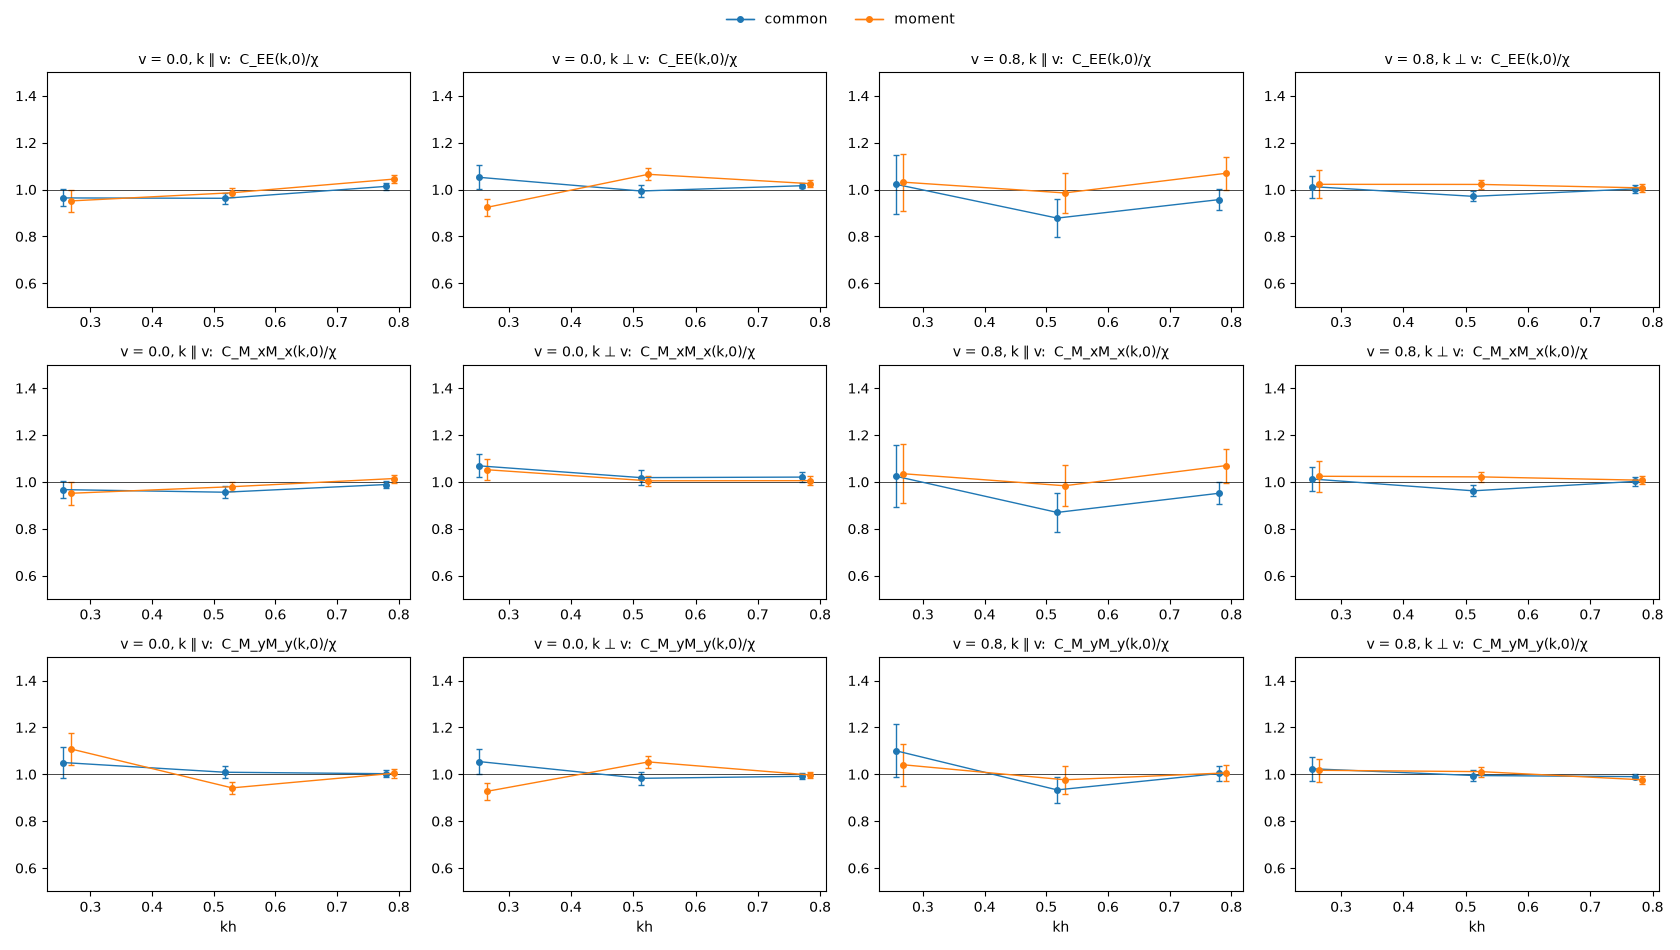
\includegraphics[width=\textwidth]{figs/moment_nersc_B_equaltime.png}
\caption{Campaign \texttt{moment\_b} ($L=1.2$, 32 runs per set): equal-time $C_{AA}(\bm k,0)/\chi_{AA}$, common and moment overlaid (key at the top).}
\label{fig:nersc_B_equaltime}
\end{figure}
\begin{figure}[p]
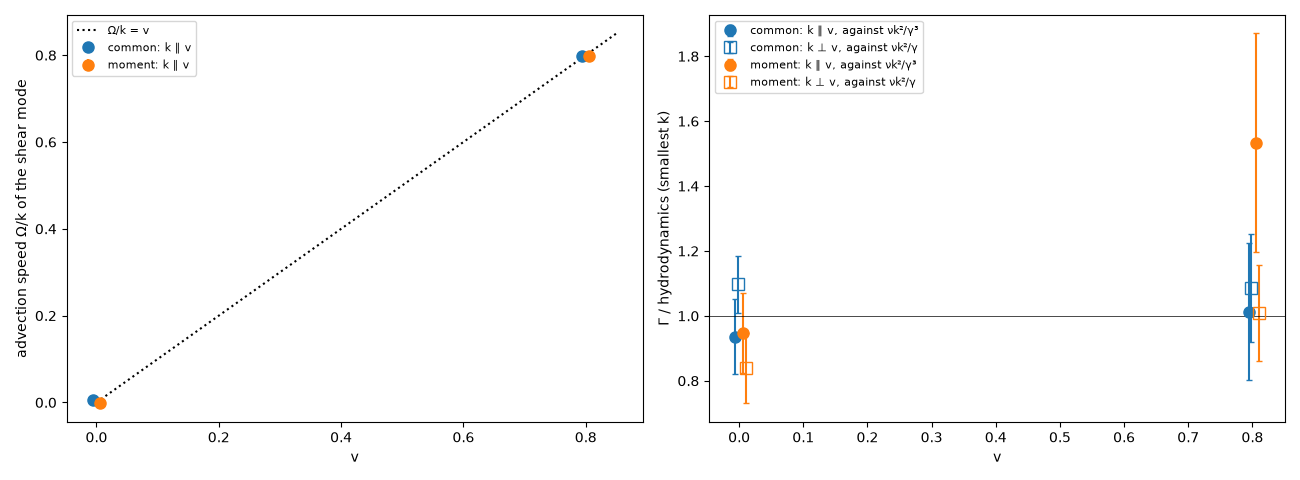
\includegraphics[width=\textwidth]{figs/moment_nersc_B_fit.png}
\caption{Campaign \texttt{moment\_b} ($L=1.2$, 32 runs per set): $\Omega/k$ and $\Gamma/\Gamma_{\rm hydro}$ of the shear mode at the smallest $k$ ($kh=0.26$) against $v_0$; common blue, moment orange; filled along, open across the flow.}
\end{figure}
\begin{figure}[p]
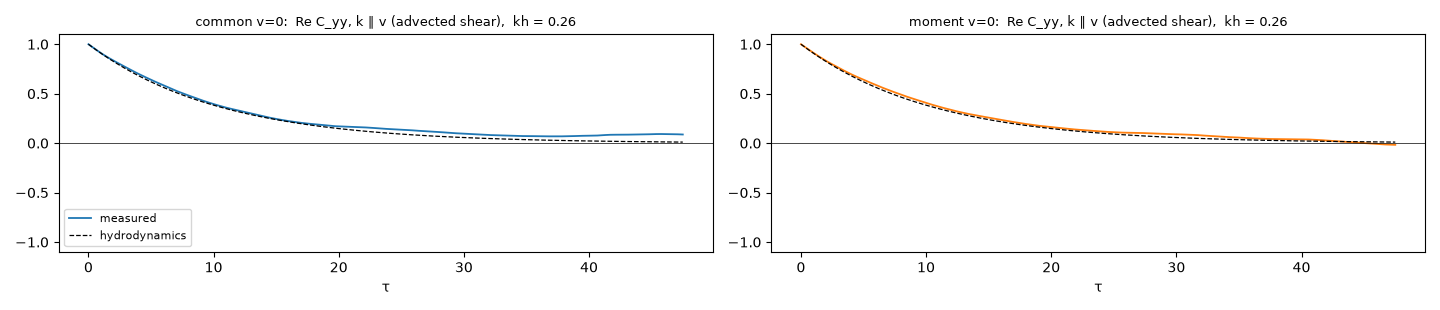
\includegraphics[width=\textwidth]{figs/moment_nersc_B_shear_v0.0.png}
\caption{Campaign \texttt{moment\_b} ($L=1.2$, 32 runs per set), at rest: the shear mode $\mathrm{Re}\,C_{yy}(k\hat x,\tau)$ at $kh=0.26$, common (left) and moment (right); dashed hydrodynamics.}
\end{figure}
\begin{figure}[p]
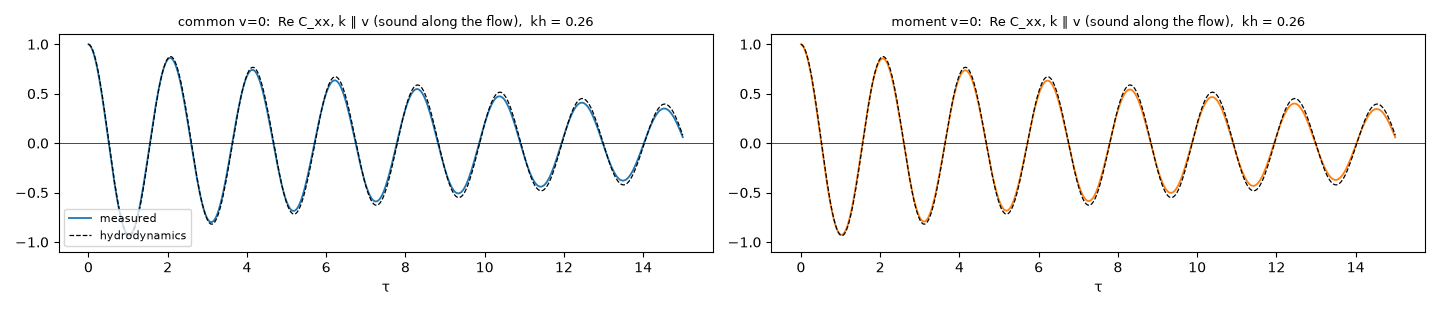
\includegraphics[width=\textwidth]{figs/moment_nersc_B_soundpar_v0.0.png}
\caption{Campaign \texttt{moment\_b} ($L=1.2$, 32 runs per set), at rest: sound, $\mathrm{Re}\,C_{xx}(k\hat x,\tau)$ at $kh=0.26$, common (left) and moment (right).}
\end{figure}
\begin{figure}[p]
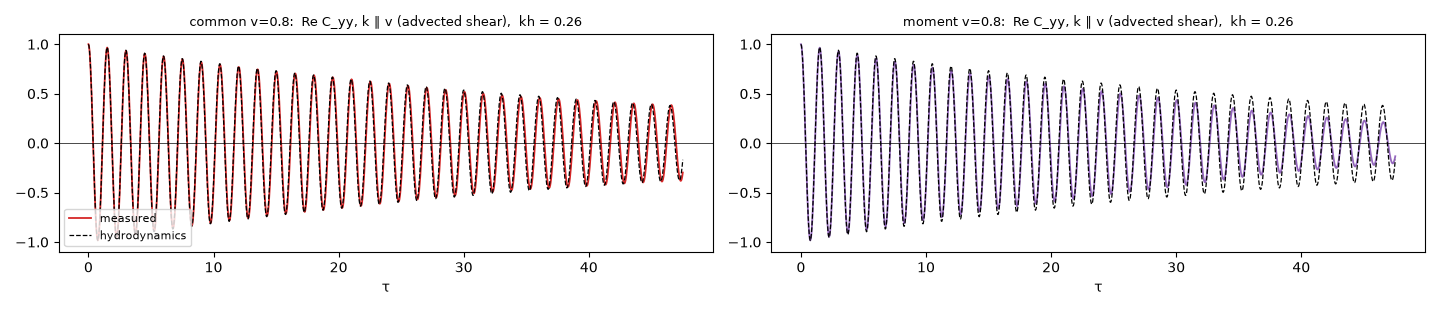
\includegraphics[width=\textwidth]{figs/moment_nersc_B_shear_v0.8.png}
\caption{Campaign \texttt{moment\_b} ($L=1.2$, 32 runs per set), $v_0=0.8$: the advected shear mode $\mathrm{Re}\,C_{yy}(k\hat x,\tau)$ at $kh=0.26$, common (left) and moment (right).}
\end{figure}
\begin{figure}[p]
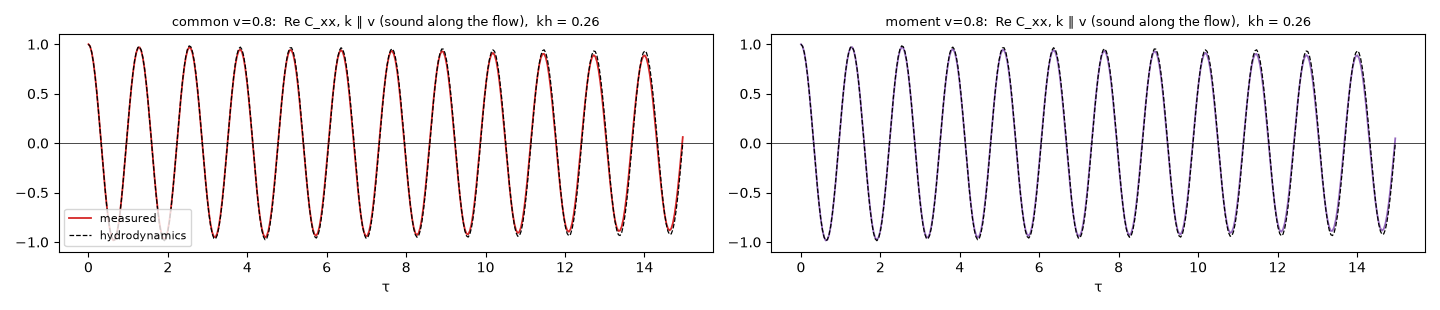
\includegraphics[width=\textwidth]{figs/moment_nersc_B_soundpar_v0.8.png}
\caption{Campaign \texttt{moment\_b} ($L=1.2$, 32 runs per set), $v_0=0.8$: sound along the flow, $\mathrm{Re}\,C_{xx}(k\hat x,\tau)$.}
\end{figure}
\begin{figure}[p]
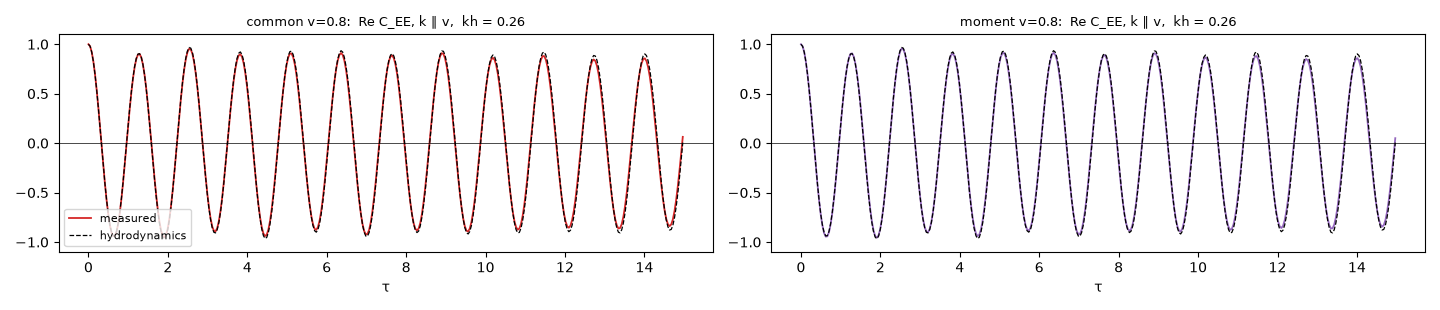
\includegraphics[width=\textwidth]{figs/moment_nersc_B_EEpar_v0.8.png}
\caption{Campaign \texttt{moment\_b} ($L=1.2$, 32 runs per set), $v_0=0.8$: $\mathrm{Re}\,C_{EE}(k\hat x,\tau)$.}
\end{figure}
\begin{figure}[p]
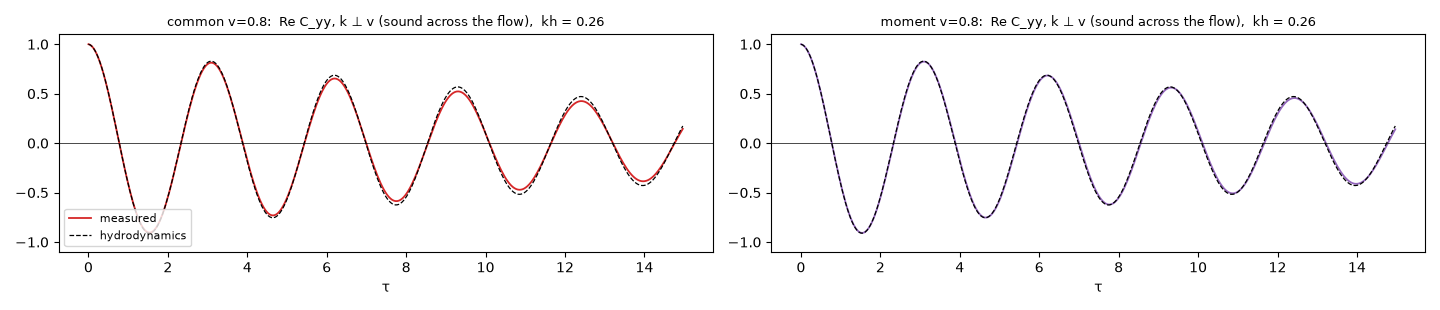
\includegraphics[width=\textwidth]{figs/moment_nersc_B_soundperp_v0.8.png}
\caption{Campaign \texttt{moment\_b} ($L=1.2$, 32 runs per set), $v_0=0.8$: sound across the flow, $\mathrm{Re}\,C_{yy}(k\hat y,\tau)$.}
\end{figure}
\begin{figure}[p]
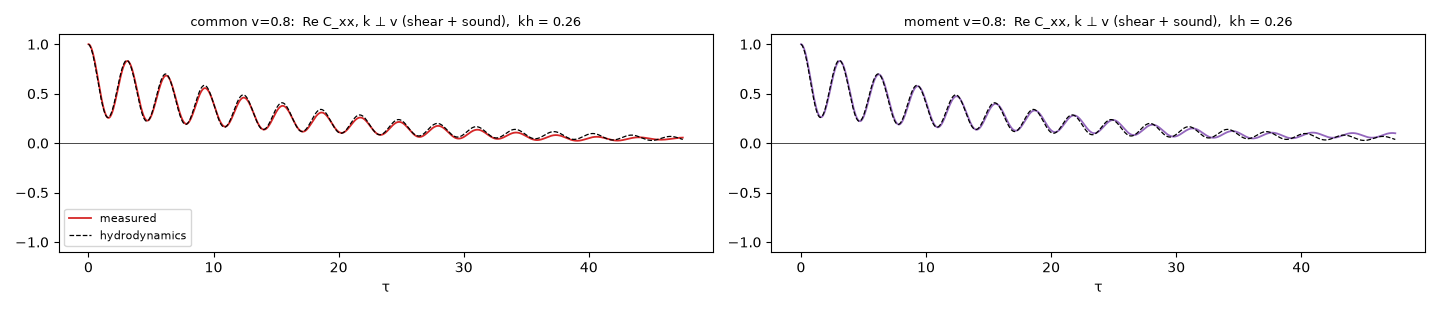
\includegraphics[width=\textwidth]{figs/moment_nersc_B_shearperp_v0.8.png}
\caption{Campaign \texttt{moment\_b} ($L=1.2$, 32 runs per set), $v_0=0.8$: across the flow, $\mathrm{Re}\,C_{xx}(k\hat y,\tau)$ (shear and sound).}
\label{fig:nersc_B_shearperp}
\end{figure}

\section{Stage 2: results from NERSC}
\label{sec:nersc2}

\emph{The answer: at rest the Hastings correction is needed --- without it the full dynamics overestimates the equal-time momentum and energy
fluctuations by about $5\%$ at $s_a=54$ and $13$--$19\%$ at $s_a=16$ against HMC of the same model; with it they agree with HMC to $1$--$2\%$.  At $v_0=0.8$
neither shows a bias within the errors ($2$--$5\%$).}

Campaign \texttt{hastings} (\texttt{nersc/campaign\_hastings.txt}, job 61364382, 8 regular nodes, 18 min; worktree at \texttt{927e035}): \texttt{moment} without
(nh) and with (h) \texttt{SPH\_HASTINGS=1}, $L=0.6$, $h/a=2$, current defaults, $s_a=16$ and $54$, $v_0=0$ and $0.8$, full step (16 runs each, $t=100$), the
stochastic step alone (8 runs, $t=50$), and HMC chains of the same model and measure (16 each, 300 updates).

\paragraph{The $\gamma$ cap and the rerun at $s_a=16$.}  20 of the 256 tasks stopped, all at $s_a=16$ without the correction, with a
\texttt{DomainError} in \texttt{sqrt\_comoving}: a particle at $|\bm v|=1$ to roundoff.  The laptop added the cap $\gamma_{\max}=100$ (\texttt{SPH\_GAMMA\_MAX},
\texttt{dfa4834}: states beyond it have no weight; the comoving structures are capped there), and all eight $s_a=16$ sets were rerun (job 61372840, 96
runs, all complete), as were the $s_a=16$ HMC chains (job 61374810).  The rerun is \emph{not} bit-identical to the first run, for the corrected runs
either: already the start differs (the HMC start and the equilibrium draw at $s_a=16$ produced states beyond $\gamma=100$, which now have no weight),
and so does the time step, set by the extreme particle ($3.1\times10^{-3}\to5.4\times10^{-3}$ at rest).  All $s_a=16$ numbers below are from the capped
runs against the capped HMC chains; the first, uncapped run is kept apart (\texttt{*\_precap}).  The $s_a=54$ sets did not come near the cap
($\max|\bm v|\le0.99$).

\paragraph{Equal-time spectra against HMC} (\texttt{examples/hastings\_analysis.jl}, \Fig{fig:hs_spectra}): $\langle|A_{\bm k}|^2\rangle/N$ of the dynamics over that of the
HMC chains, in bands $kh=0.52$--$1.56$, errors from the spread of the runs:
\begin{center}
\resizebox{\textwidth}{!}{\begin{tabular}{lcc}
\hline
 & without & with the correction \\ \hline
$s_a=54$, $v_0=0$: $M_L$, $M_T$, $E$ & $1.02$--$1.06$, $1.02$--$1.08$, $1.05$--$1.06$ ($2$--$5\sigma$) & $1.00\pm0.01$ in all three \\
$s_a=16$, $v_0=0$: $M_L$, $M_T$, $E$ & $1.16$--$1.19$, $1.16$--$1.18$, $1.13$--$1.15$ ($5$--$18\sigma$); alone $1.16$--$1.22$ & $0.98$--$1.02$; alone $0.99$--$1.06$ \\
$s_a=54$, $v_0=0.8$ & $1$ within the errors (one band $0.88(9)$) & $1$ within the errors \\
$s_a=16$, $v_0=0.8$ & $1$ within the errors & $1$ within the errors (one band $0.85(6)$) \\
\hline
\end{tabular}}
\end{center}
(For the stochastic step alone at $v_0=0.8$ the HMC chains are not the reference --- the alone runs keep the positions of their start --- and
both versions scatter alike.)

\paragraph{Acceptances and rejections} (from the running totals in the task logs, mean over the runs; $s_a=16$ from the capped rerun).  ``nh'' without, ``h'' with the correction; ``light cone'' the fraction of proposals rejected because a
particle would reach $|\bm v|\ge1$:
\begin{center}
\resizebox{\textwidth}{!}{\begin{tabular}{llccccc}
\hline
set & runs (complete) & stress acc., nh / h & residual acc., nh / h & $\Delta$ residual & light cone, residual, nh / h \\ \hline
$s_a=16$, $v_0=0$, full & $16$ / $16$ & $0.917$ / $0.920$ & $0.644$ / $0.441$ & $-0.20$ & $0.12$ / $0.10$ \\
$s_a=16$, $v_0=0$, alone & $8$ / $8$ & $0.920$ / $0.923$ & $0.623$ / $0.408$ & $-0.22$ & $0.11$ / $0.10$ \\
$s_a=16$, $v_0=0.8$, full & $16$ / $16$ & $0.970$ / $0.969$ & $0.835$ / $0.541$ & $-0.29$ & $9\times10^{-3}$ / $7\times10^{-3}$ \\
$s_a=16$, $v_0=0.8$, alone & $8$ / $8$ & $0.970$ / $0.968$ & $0.835$ / $0.534$ & $-0.30$ & $8\times10^{-3}$ / $8\times10^{-3}$ \\
$s_a=54$, $v_0=0$, full & $16$ / $16$ & $0.951$ / $0.952$ & $0.660$ / $0.622$ & $-0.04$ & $8\times10^{-5}$ / $5\times10^{-5}$ \\
$s_a=54$, $v_0=0$, alone & $8$ / $8$ & $0.952$ / $0.952$ & $0.664$ / $0.625$ & $-0.04$ & $5\times10^{-5}$ / $4\times10^{-5}$ \\
$s_a=54$, $v_0=0.8$, full & $16$ / $16$ & $0.970$ / $0.970$ & $0.817$ / $0.644$ & $-0.17$ & $10^{-7}$ / $4\times10^{-8}$ \\
$s_a=54$, $v_0=0.8$, alone & $8$ / $8$ & $0.970$ / $0.970$ & $0.817$ / $0.644$ & $-0.17$ & $4\times10^{-8}$ / $4\times10^{-8}$ \\
\hline
\end{tabular}}
\end{center}
The correction leaves the stress move alone (the acceptances agree to $10^{-3}$) and rejects residual moves: $4\%$ more at $s_a=54$ at rest, $17\%$
in the moving fluid, $20$--$30\%$ at $s_a=16$.  The full step and the stochastic step alone lose the same amount, so the extra rejections belong to
the stochastic step, not to its coupling with the ideal step.  The light-cone rejections are large only at $s_a=16$ at rest ($3\%$ of the stress and
$11\%$ of the residual proposals), and the same without and with the correction.

\paragraph{The log ratios} $\ln q'/q$ of the corrected runs (recorded per window: the mean and rms over the proposals of a sweep; medians and
quantiles over the windows of all runs):
\begin{center}
\resizebox{\textwidth}{!}{\begin{tabular}{lrcccccc}
\hline
set & windows & stress: mean & stress: rms & residual: mean (10\%, 90\%) & residual: rms & rms $>10$ & rms $>100$ \\ \hline
$s_a=16$, $v_0=0$, full & $109\,216$ & $-1.1\times10^{-3}$ & $0.041$ & $-63$ ($-1.8\times10^4$, $-4.1$) & $2.1\times10^3$ & $100\%$ & $84\%$ \\
$s_a=16$, $v_0=0$, alone & $20\,138$ & $-1.6\times10^{-3}$ & $0.049$ & $-305$ ($-8.3\times10^4$, $-19$) & $1.2\times10^4$ & $100\%$ & $98\%$ \\
$s_a=16$, $v_0=0.8$, full & $197\,085$ & $-3.4\times10^{-4}$ & $0.029$ & $-1.44$ ($-2.24$, $-0.41$) & $4.8$ & $14\%$ & $1.8\%$ \\
$s_a=16$, $v_0=0.8$, alone & $44\,995$ & $-4.2\times10^{-4}$ & $0.031$ & $-1.73$ ($-2.22$, $-0.84$) & $5.6$ & $16\%$ & $1.9\%$ \\
$s_a=54$, $v_0=0$, full & $46\,192$ & $-9.6\times10^{-5}$ & $0.007$ & $-0.36$ ($-0.44$, $-0.31$) & $1.8$ & $2.6\%$ & $0.4\%$ \\
$s_a=54$, $v_0=0$, alone & $11\,802$ & $-9.0\times10^{-5}$ & $0.007$ & $-0.35$ ($-0.42$, $-0.29$) & $1.8$ & $1.8\%$ & $0.2\%$ \\
$s_a=54$, $v_0=0.8$, full & $76\,976$ & $-7.4\times10^{-5}$ & $0.013$ & $-0.54$ ($-0.58$, $-0.50$) & $1.6$ & $0$ & $0$ \\
$s_a=54$, $v_0=0.8$, alone & $19\,240$ & $-7.2\times10^{-5}$ & $0.013$ & $-0.54$ ($-0.58$, $-0.50$) & $1.6$ & $0$ & $0$ \\
\hline
\end{tabular}}
\end{center}
The stress ratios are tiny everywhere.  The residual ratios are of order one at $s_a=54$ and at $s_a=16$ in the moving fluid, with a negative mean
(the reason for the extra rejections), and rare large windows.  At $s_a=16$ at rest they are large in almost every window (median rms $2.1\times10^3$,
maxima $\sim10^{13}$ with the cap, $\sim10^{18}$ before): residual covariances close to singular in many stars.  The spectra still agree with HMC there, but the residual move is then
decided by $q'/q$ rather than by $\Delta S$.

\paragraph{Kinetic energy and damping} (\texttt{boost\_analysis.jl}, groups HS54, HS16; Figs.~\ref{fig:hs54_et}--\ref{fig:hs16_last}).  KE$/2VwT$ against the
continuum, without / with the correction: $s_a=54$: $0.987$ / $0.948$ at rest, $16.80$ / $16.37$ at $v_0=0.8$; $s_a=16$: $0.972$ / $0.849$ and $15.55$ / $14.20$.  The
corrected values are lower, as is the HMC equilibrium of the same model at finite $s_a$.
\begin{center}
\resizebox{\textwidth}{!}{\begin{tabular}{lcccc}
\hline
shear $\Gamma/\Gamma_{\rm hydro}$, without / with & at rest, $kh=0.52$, $\bm k$ along $x$, $y$ & at rest, $kh=1.05$, $x$, $y$ & $v_0=0.8$, $kh=0.52$, along, across & $v_0=0.8$, $kh=1.05$, along, across \\ \hline
$s_a=54$ & $0.92(8)$, $0.99(7)$ / $0.95(7)$, $1.10(6)$ & $1.00(4)$, $1.04(4)$ / $1.11(2)$, $1.05(2)$ & $1.33(18)$, $1.20(13)$ / $1.13(15)$, $1.20(9)$ & $1.22(8)$, $1.17(4)$ / $1.20(8)$, $0.97(4)$ \\
$s_a=16$$^\ddagger$ & $0.93(4)$, $0.96(5)$ / $1.08(6)$, $1.04(5)$ & $0.96(3)$, $0.90(2)$ / $1.10(3)$, $1.04(3)$ & $1.02(15)$, $1.25(7)$ / $1.06(10)$, $1.22(9)$ & $1.17(7)$, $1.18(4)$ / $1.11(5)$, $1.07(3)$ \\
\hline
\end{tabular}}
\end{center}
$^\ddagger$\,The row $s_a=16$ is that of the corrected analysis (\Sect{sec:lagfix}); the first version of this note had $2.6$ and $2.4$ along the flow at
$kh=0.52$, an artifact of runs with different time steps.  At $s_a=16$ at rest the corrected dynamics damps the shear mode $\approx15\%$ faster than the
uncorrected one ($1.04$--$1.10$ against $0.90$--$0.96$, about $2\sigma$ per fit, the same in all four); at $s_a=54$ the same tendency is weaker.  In motion
at $s_a=16$ both are within $1.0$--$1.25$ of hydrodynamics.
$\Delta H/H$: $2\times10^{-5}$--$2.5\times10^{-4}$ at $s_a=54$, $2\times10^{-4}$--$2\times10^{-3}$ at $16$.

\begin{figure}[p]
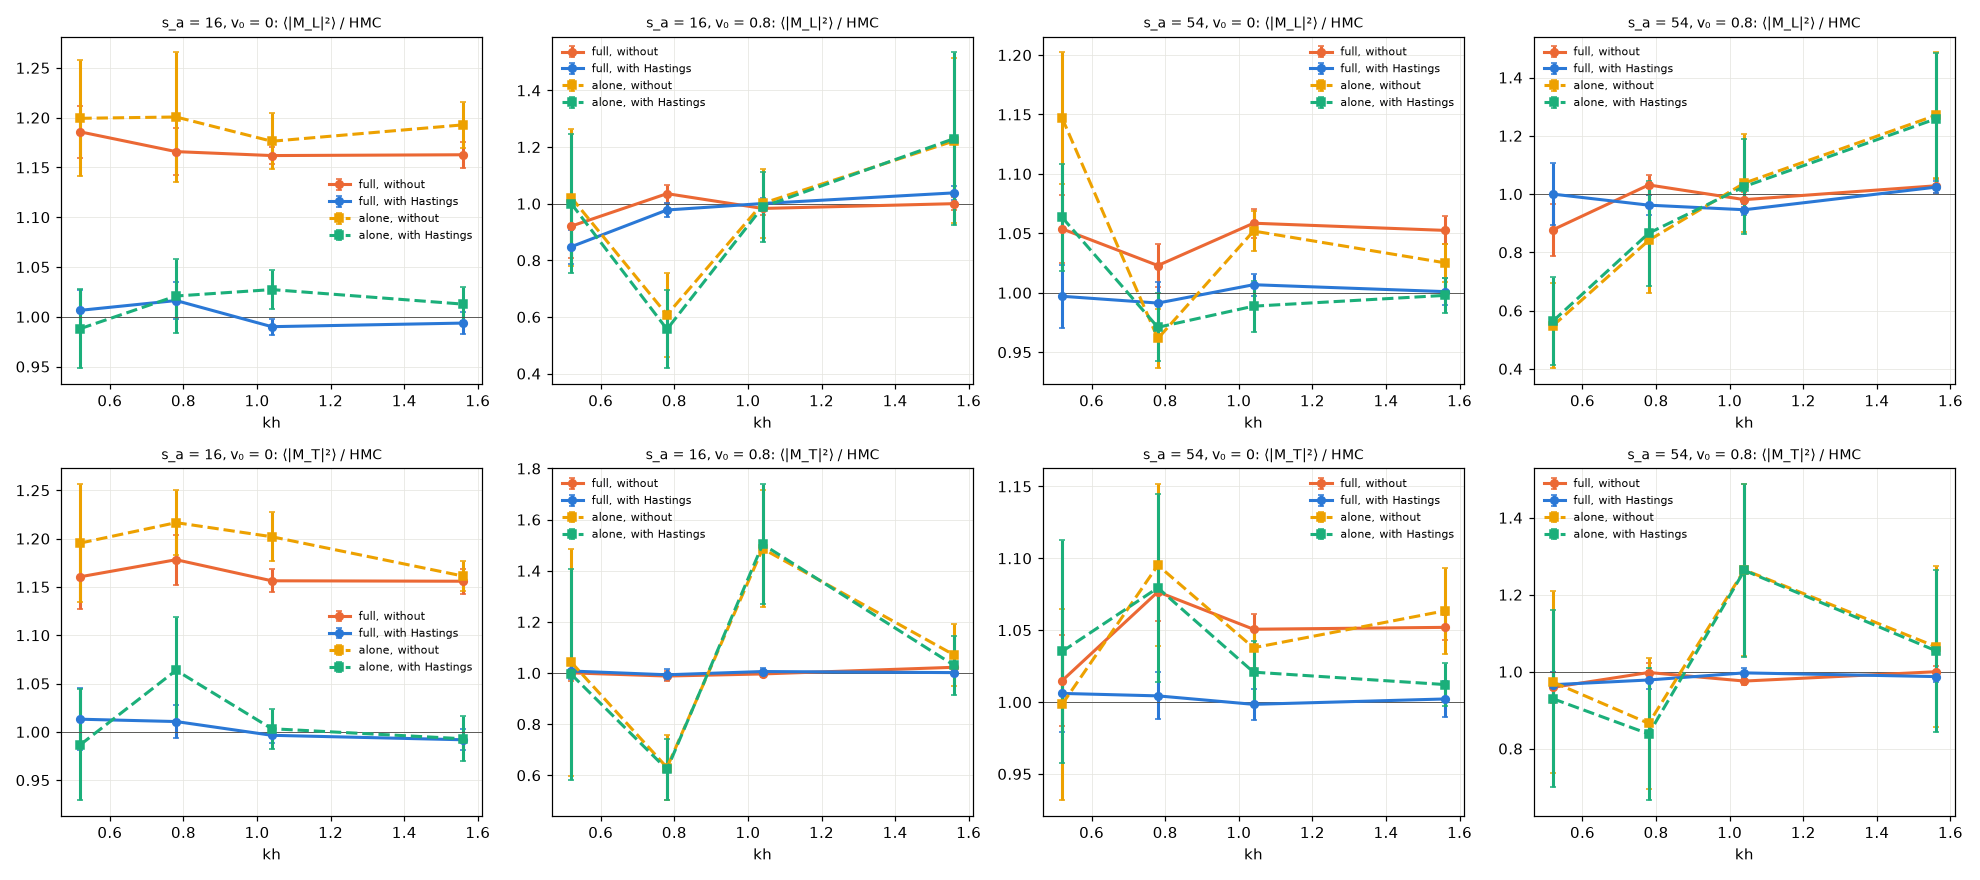
\includegraphics[width=\textwidth]{figs/hastings_nersc_spectra.png}
\caption{Campaign \texttt{hastings}: equal-time $\langle|M_L|^2\rangle$ (top) and $\langle|M_T|^2\rangle$ (bottom) of the dynamics over HMC of the same model, against $kh$; full step without (orange) and with (blue) the correction, the stochastic step alone without (yellow) and with (green); $s_a=16$, $54$ at $v_0=0$, $0.8$ (columns).  \texttt{examples/hastings\_analysis.jl}.}
\label{fig:hs_spectra}
\end{figure}
\begin{figure}[p]
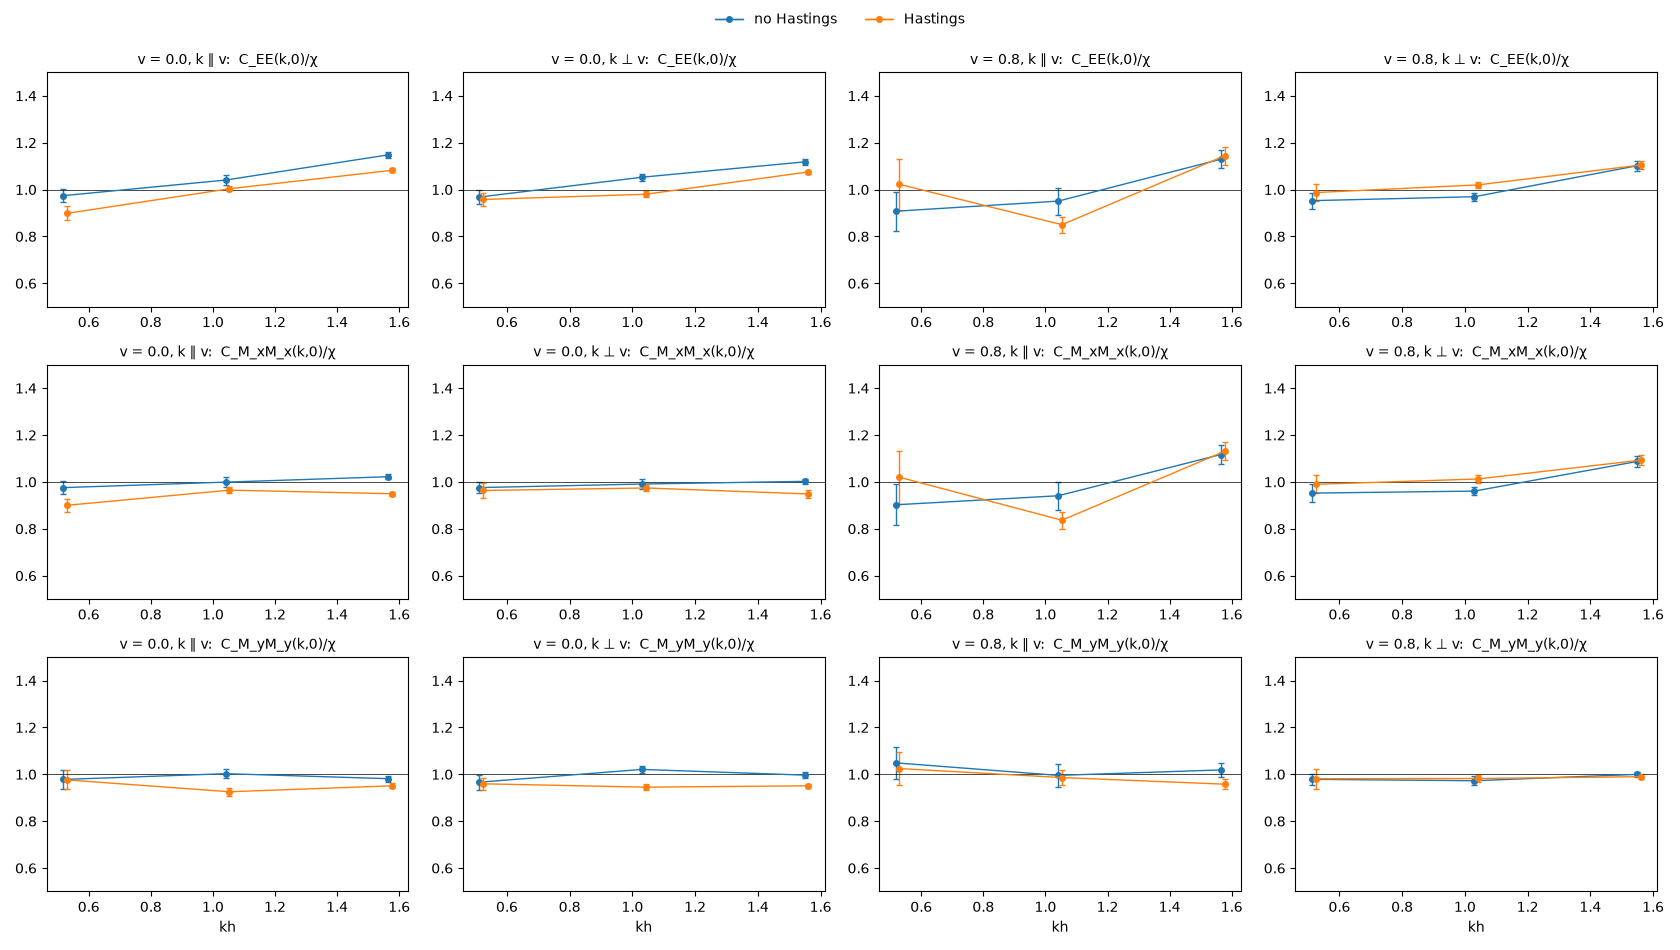
\includegraphics[width=\textwidth]{figs/hastings_nersc_HS54_equaltime.png}
\caption{$s_a=54$: equal-time $C_{AA}(\bm k,0)/\chi_{AA}$, without and with the correction (key at the top); 16 runs each.}
\label{fig:hs54_et}
\end{figure}
\begin{figure}[p]
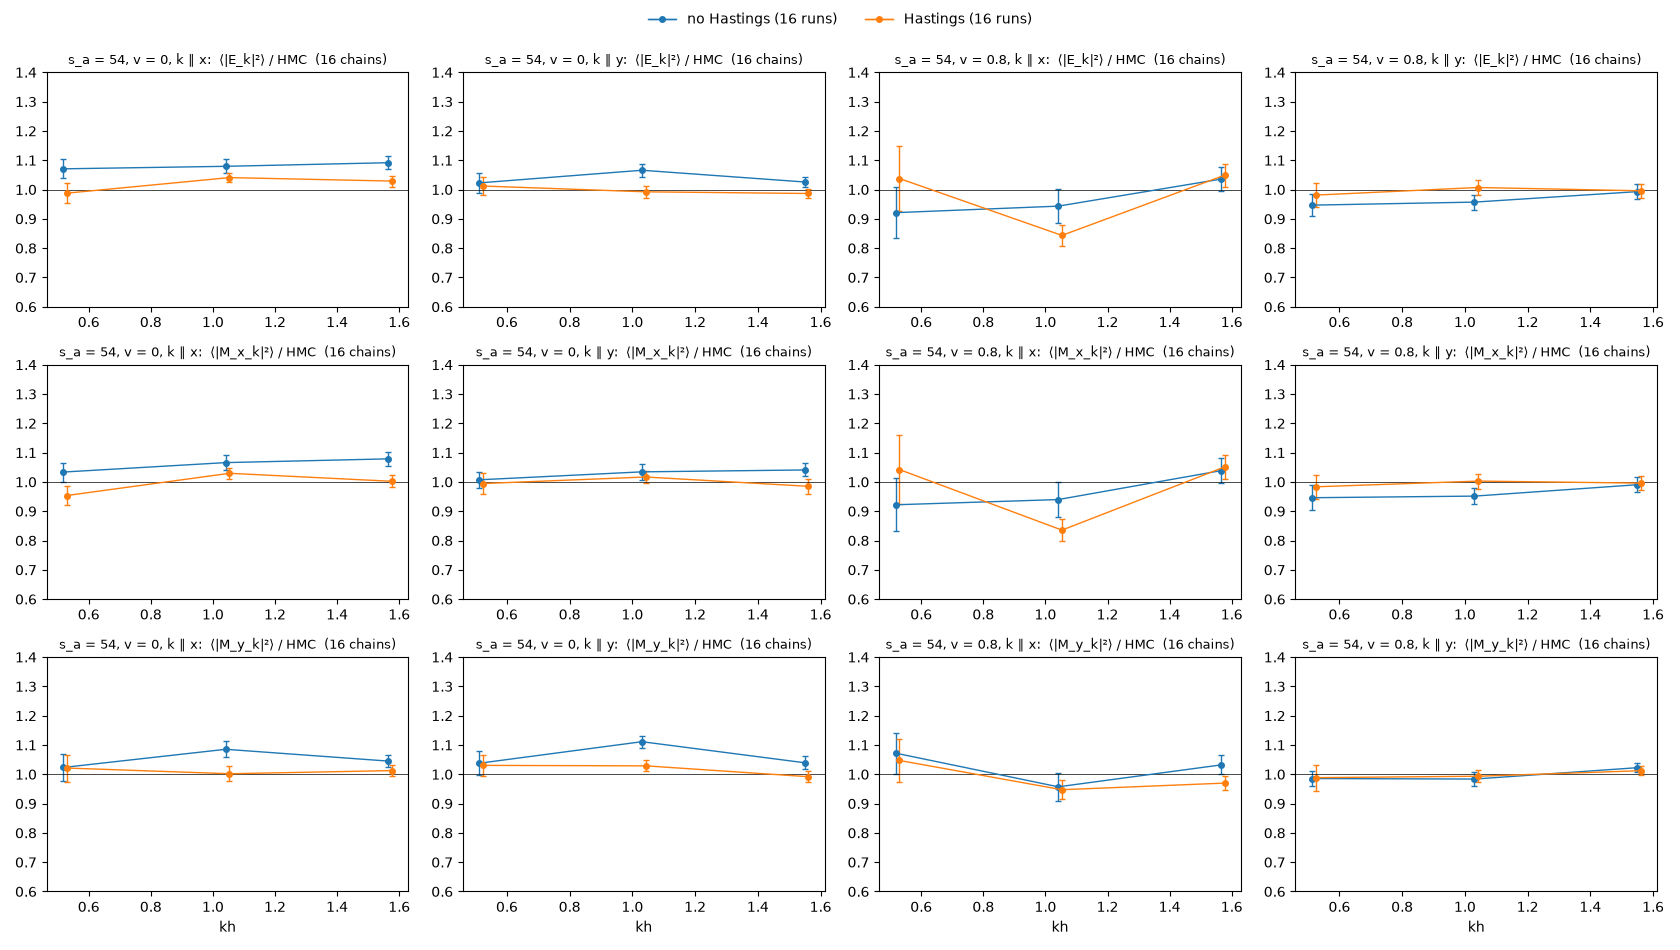
\includegraphics[width=\textwidth]{figs/hastings_nersc_HS54_equaltime_hmc.png}
\caption{$s_a=54$: as \Fig{fig:hs54_et}, the equal-time $\langle|A_{\bm k}|^2\rangle$ divided by HMC of the same model and measure instead of by $\chi$ (16 runs,
16 chains each; the three smallest modes along $x$ and $y$).  At rest the runs without the correction lie $2$--$11\%$ above HMC, with it on $1$.
\texttt{examples/equaltime\_over\_hmc.jl}.}
\label{fig:hs54_et_hmc}
\end{figure}
\begin{figure}[p]
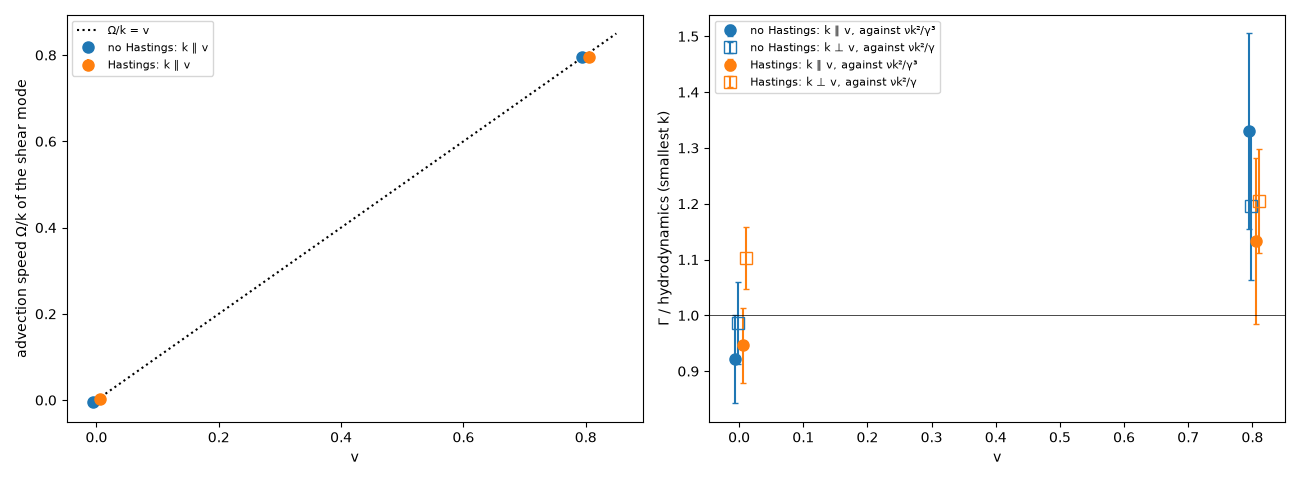
\includegraphics[width=\textwidth]{figs/hastings_nersc_HS54_fit.png}
\caption{$s_a=54$: $\Omega/k$ and $\Gamma/\Gamma_{\rm hydro}$ of the shear mode at $kh=0.52$ against $v_0$, without (blue) and with (orange) the correction; filled along, open across.}
\end{figure}
\begin{figure}[p]
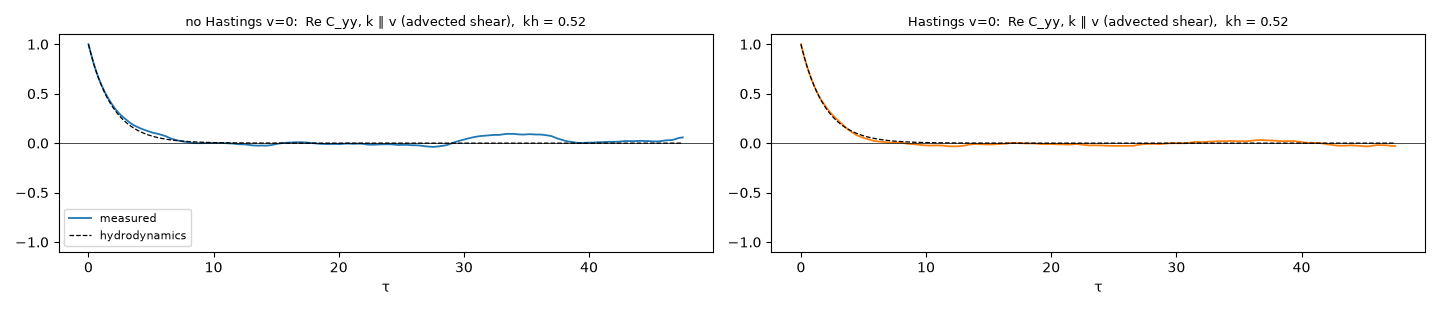
\includegraphics[width=\textwidth]{figs/hastings_nersc_HS54_shear_v0.0.png}
\caption{$s_a=54$, at rest: the shear mode $\mathrm{Re}\,C_{yy}(k\hat x,\tau)$ at $kh=0.52$; without (left) and with (right) the correction; dashed hydrodynamics.}
\end{figure}
\begin{figure}[p]
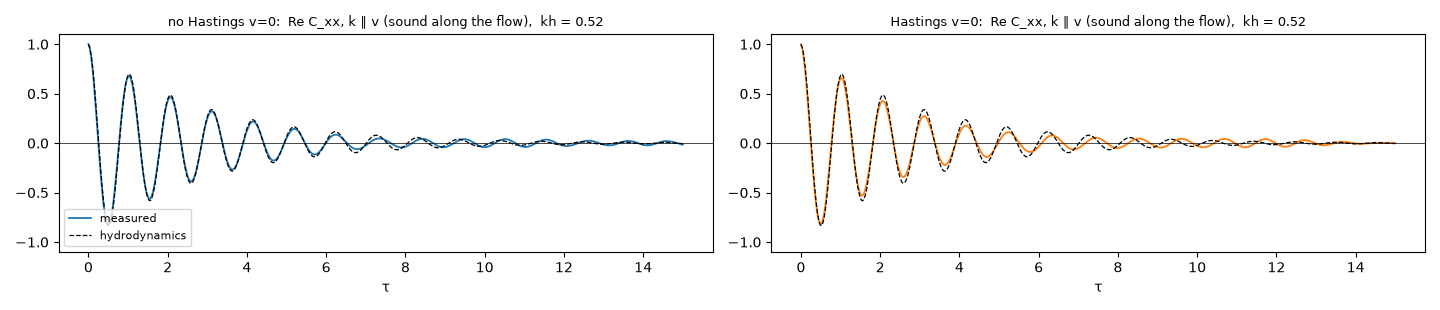
\includegraphics[width=\textwidth]{figs/hastings_nersc_HS54_soundpar_v0.0.png}
\caption{$s_a=54$, at rest: sound, $\mathrm{Re}\,C_{xx}(k\hat x,\tau)$; without (left) and with (right) the correction; dashed hydrodynamics.}
\end{figure}
\begin{figure}[p]
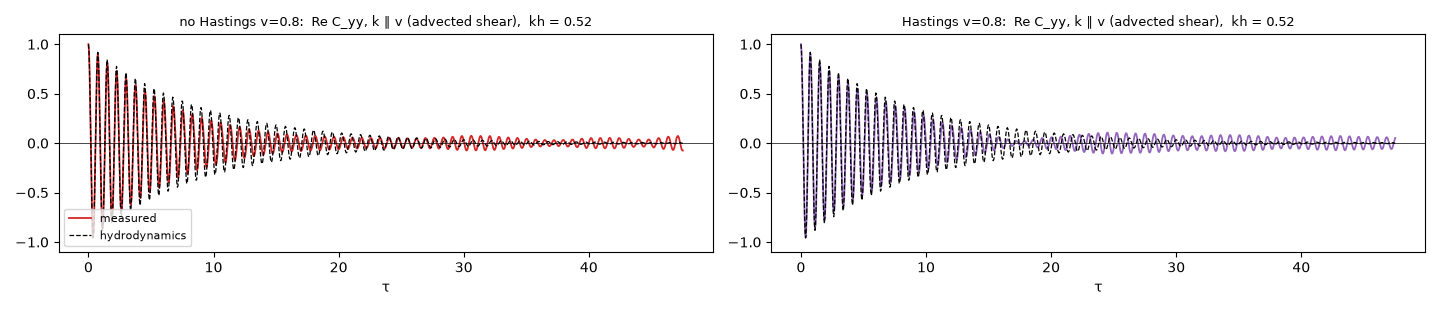
\includegraphics[width=\textwidth]{figs/hastings_nersc_HS54_shear_v0.8.png}
\caption{$s_a=54$, $v_0=0.8$: the advected shear mode $\mathrm{Re}\,C_{yy}(k\hat x,\tau)$; without (left) and with (right) the correction; dashed hydrodynamics.}
\end{figure}
\begin{figure}[p]
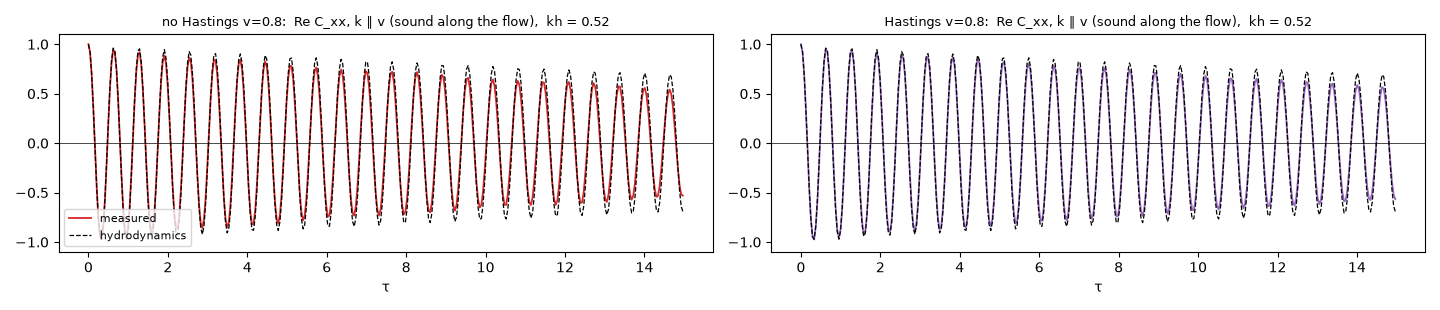
\includegraphics[width=\textwidth]{figs/hastings_nersc_HS54_soundpar_v0.8.png}
\caption{$s_a=54$, $v_0=0.8$: sound along the flow, $\mathrm{Re}\,C_{xx}(k\hat x,\tau)$; without (left) and with (right) the correction; dashed hydrodynamics.}
\end{figure}
\begin{figure}[p]
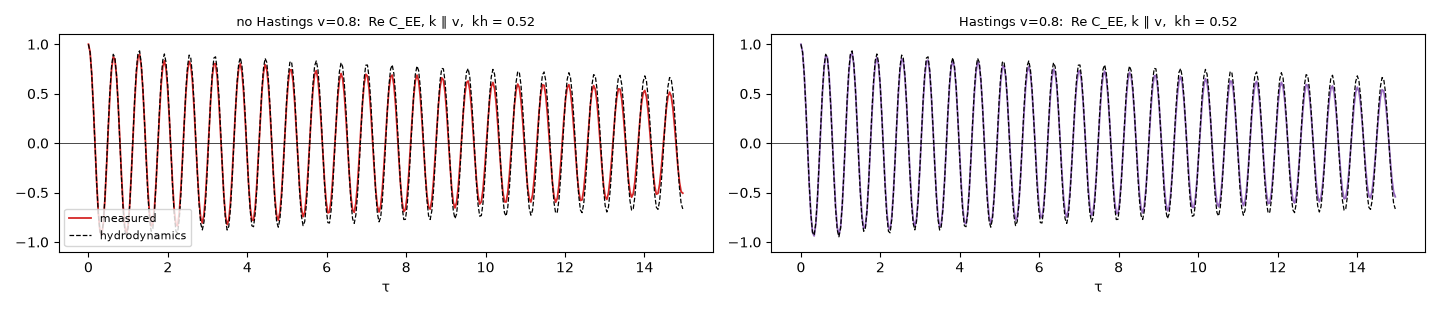
\includegraphics[width=\textwidth]{figs/hastings_nersc_HS54_EEpar_v0.8.png}
\caption{$s_a=54$, $v_0=0.8$: $\mathrm{Re}\,C_{EE}(k\hat x,\tau)$; without (left) and with (right) the correction; dashed hydrodynamics.}
\end{figure}
\begin{figure}[p]
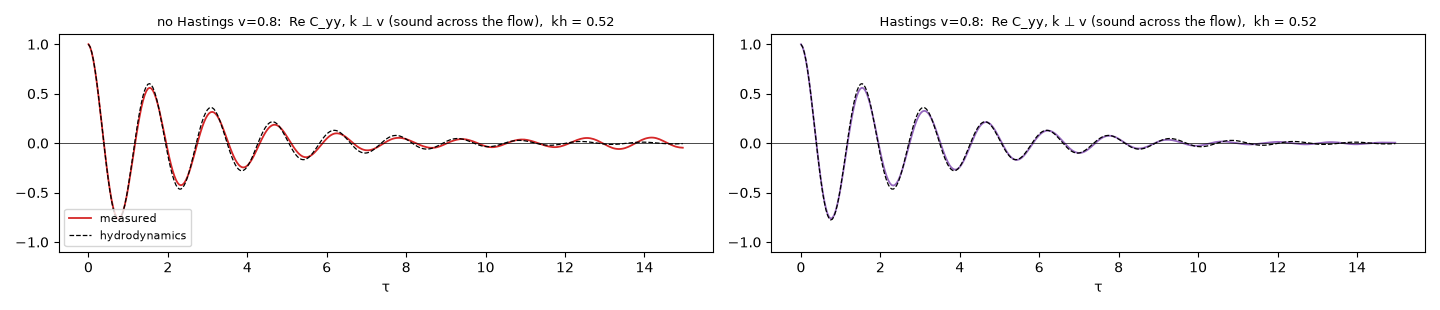
\includegraphics[width=\textwidth]{figs/hastings_nersc_HS54_soundperp_v0.8.png}
\caption{$s_a=54$, $v_0=0.8$: sound across the flow, $\mathrm{Re}\,C_{yy}(k\hat y,\tau)$; without (left) and with (right) the correction; dashed hydrodynamics.}
\end{figure}
\begin{figure}[p]
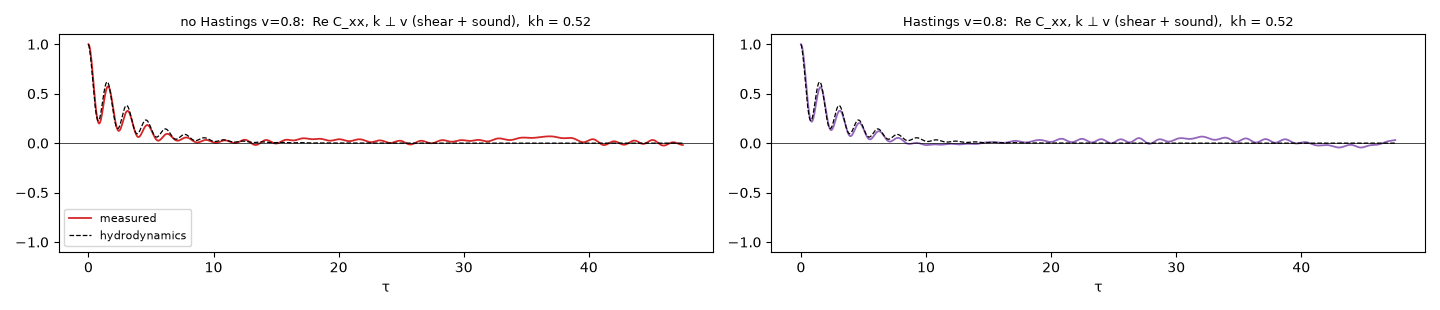
\includegraphics[width=\textwidth]{figs/hastings_nersc_HS54_shearperp_v0.8.png}
\caption{$s_a=54$, $v_0=0.8$: across the flow, $\mathrm{Re}\,C_{xx}(k\hat y,\tau)$ (shear and sound); without (left) and with (right) the correction; dashed hydrodynamics.}
\end{figure}
\begin{figure}[p]
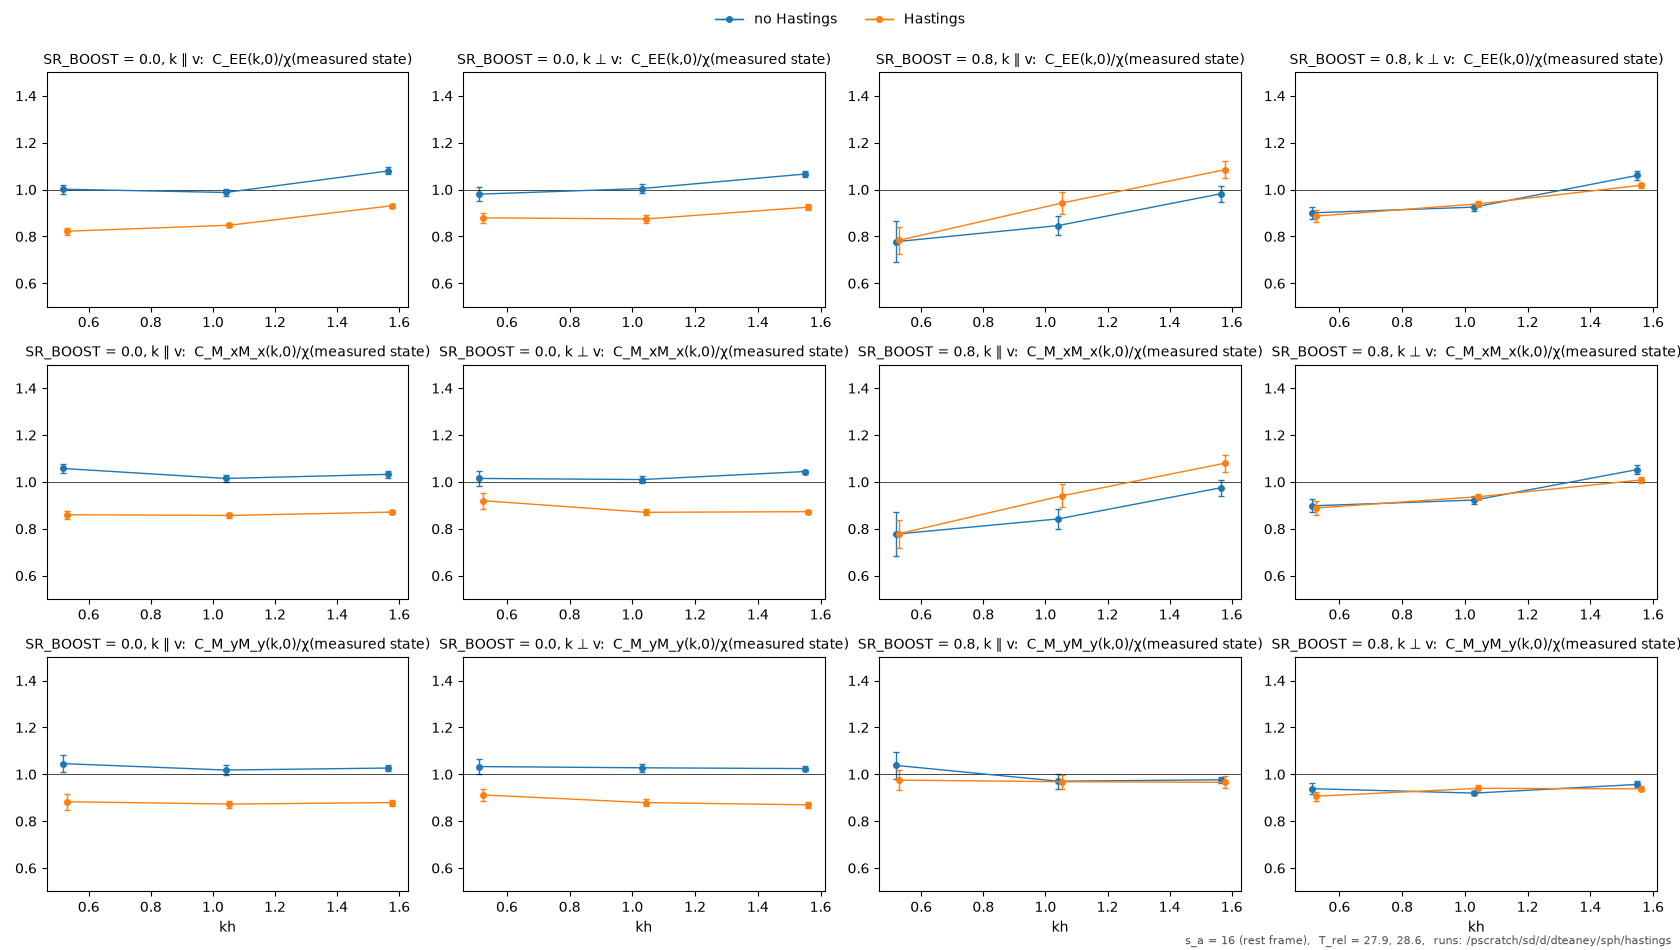
\includegraphics[width=\textwidth]{figs/hastings_nersc_HS16_equaltime.png}
\caption{$s_a=16$ (capped rerun): equal-time $C_{AA}(\bm k,0)/\chi_{AA}$, without and with the correction (key at the top); 16 runs each.}
\label{fig:hs16_et}
\end{figure}
\begin{figure}[p]
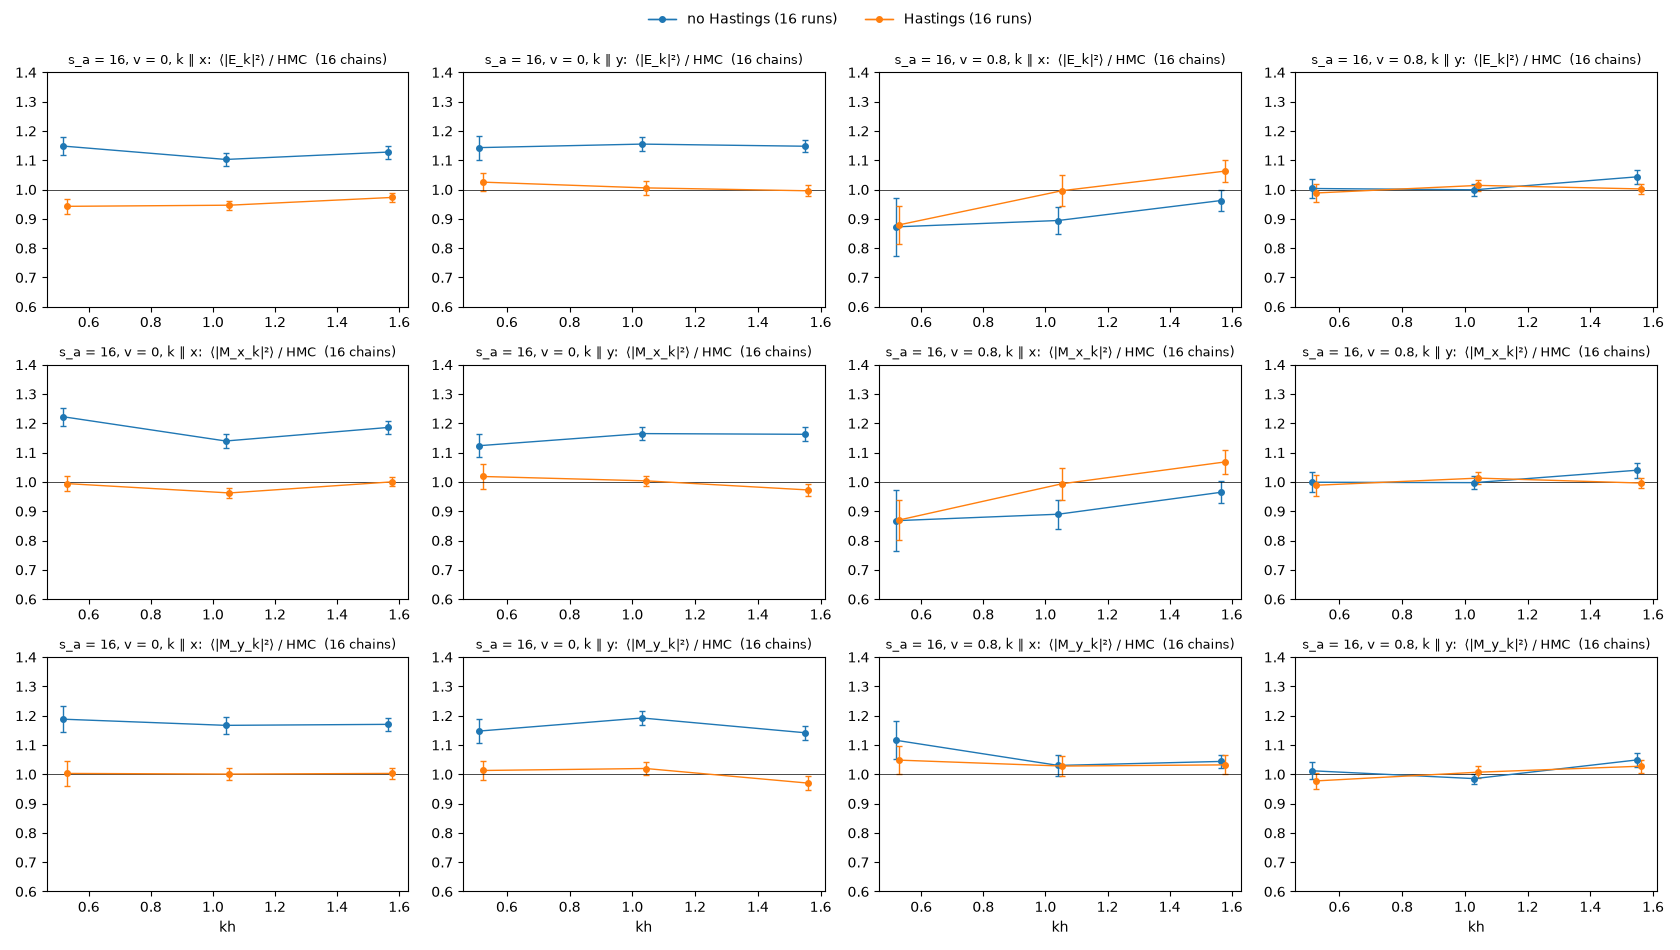
\includegraphics[width=\textwidth]{figs/hastings_nersc_HS16_equaltime_hmc.png}
\caption{$s_a=16$: as \Fig{fig:hs16_et}, divided by HMC of the same model and measure (16 capped chains) instead of by $\chi$.  At rest the runs without the correction lie $10$--$22\%$ above HMC, with it on $1$.  \texttt{examples/equaltime\_over\_hmc.jl}.}
\end{figure}
\begin{figure}[p]
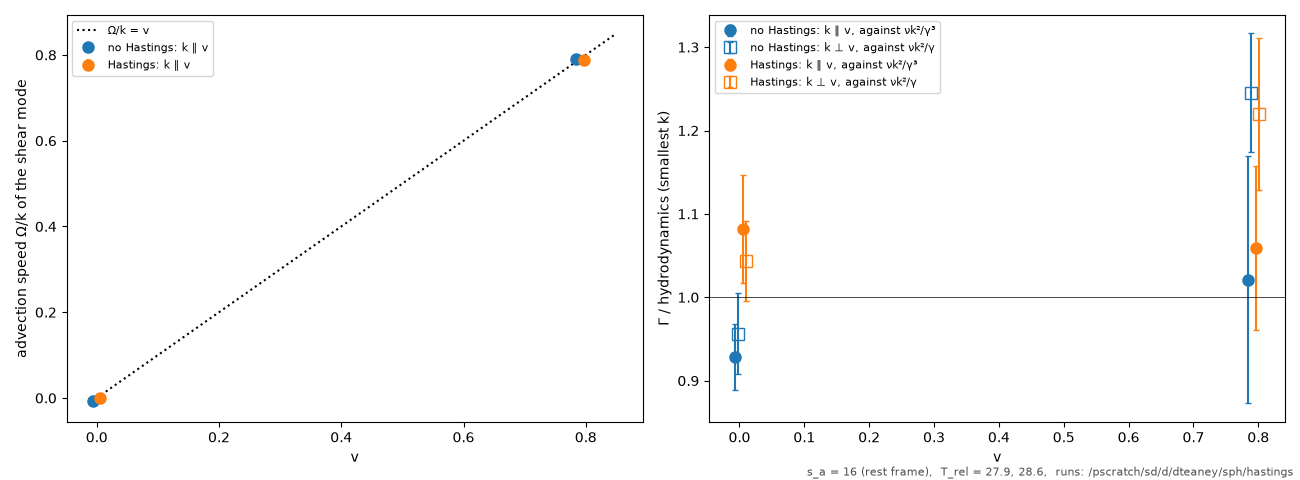
\includegraphics[width=\textwidth]{figs/hastings_nersc_HS16_fit.png}
\caption{$s_a=16$: $\Omega/k$ and $\Gamma/\Gamma_{\rm hydro}$ of the shear mode at $kh=0.52$ against $v_0$, without (blue) and with (orange) the correction; filled along, open across.}
\end{figure}
\begin{figure}[p]
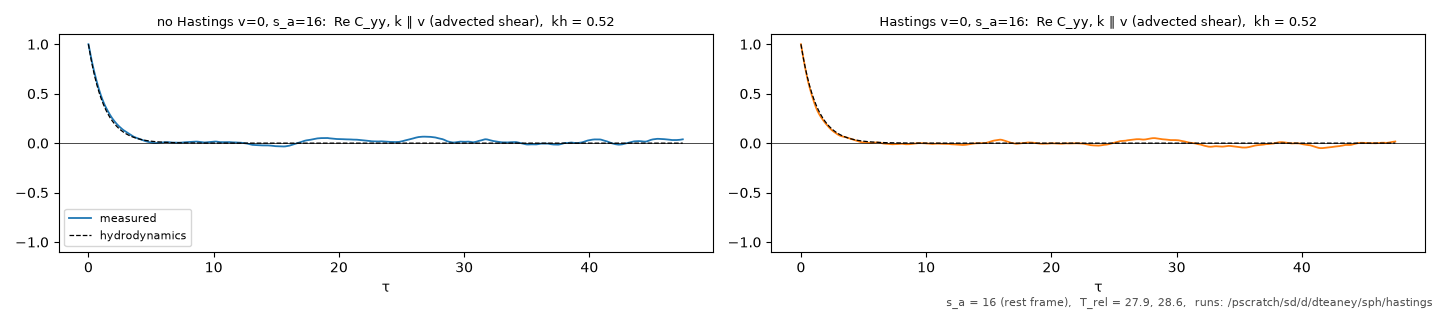
\includegraphics[width=\textwidth]{figs/hastings_nersc_HS16_shear_v0.0.png}
\caption{$s_a=16$, at rest: the shear mode $\mathrm{Re}\,C_{yy}(k\hat x,\tau)$ at $kh=0.52$; without (left) and with (right) the correction; dashed hydrodynamics.}
\end{figure}
\begin{figure}[p]
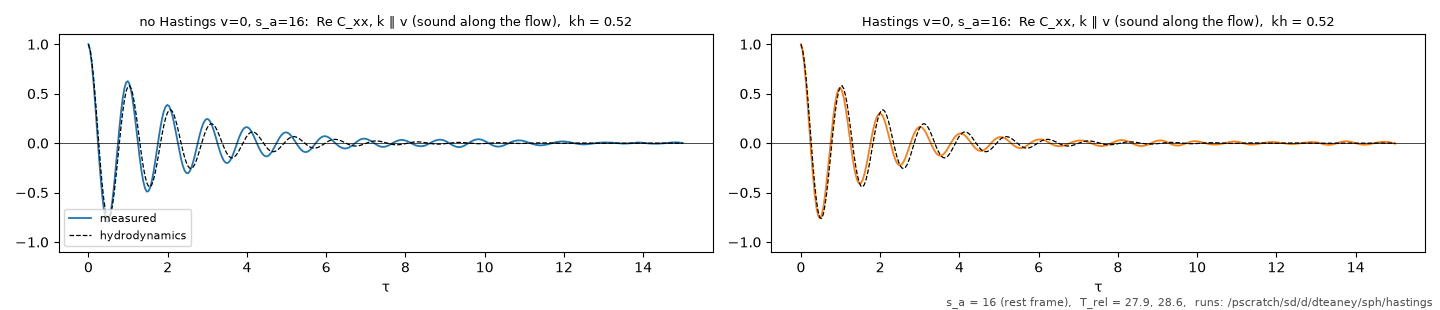
\includegraphics[width=\textwidth]{figs/hastings_nersc_HS16_soundpar_v0.0.png}
\caption{$s_a=16$, at rest: sound, $\mathrm{Re}\,C_{xx}(k\hat x,\tau)$; without (left) and with (right) the correction; dashed hydrodynamics.}
\end{figure}
\begin{figure}[p]
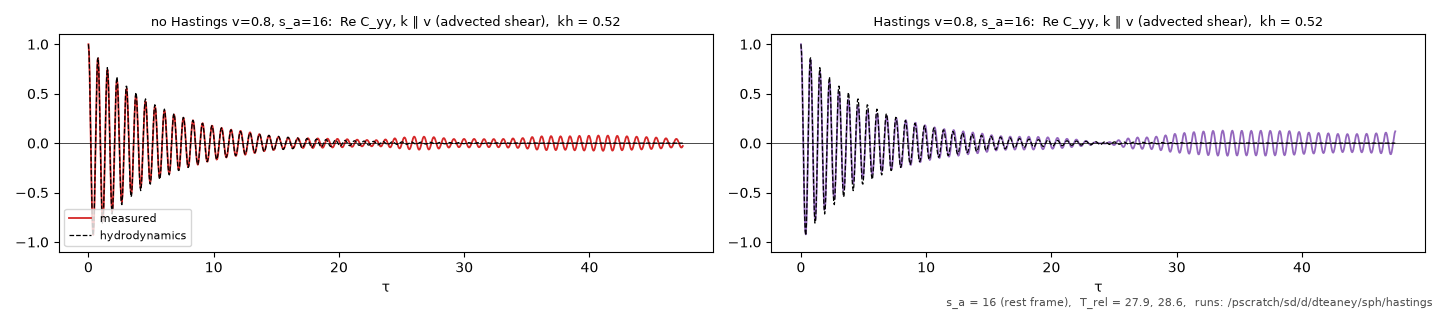
\includegraphics[width=\textwidth]{figs/hastings_nersc_HS16_shear_v0.8.png}
\caption{$s_a=16$, $v_0=0.8$: the advected shear mode $\mathrm{Re}\,C_{yy}(k\hat x,\tau)$ (far from hydrodynamics in both); without (left) and with (right) the correction; dashed hydrodynamics.}
\end{figure}
\begin{figure}[p]
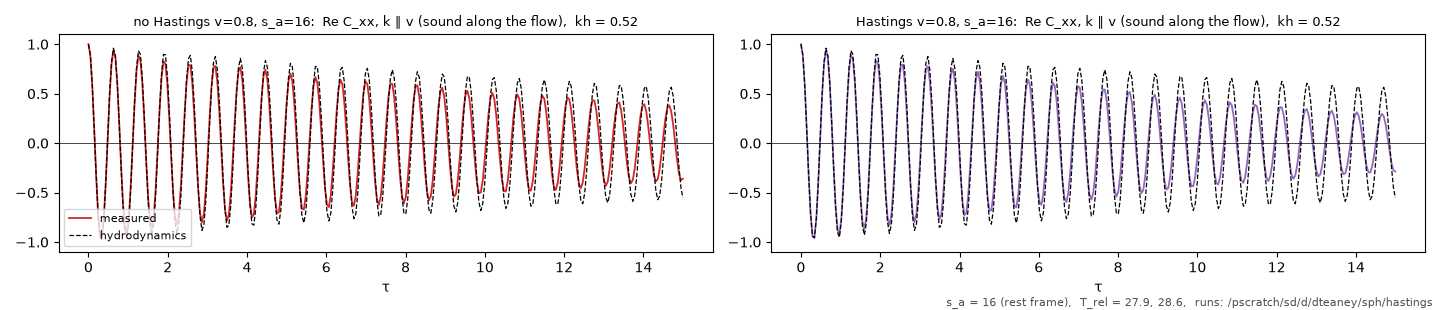
\includegraphics[width=\textwidth]{figs/hastings_nersc_HS16_soundpar_v0.8.png}
\caption{$s_a=16$, $v_0=0.8$: sound along the flow, $\mathrm{Re}\,C_{xx}(k\hat x,\tau)$; without (left) and with (right) the correction; dashed hydrodynamics.}
\end{figure}
\begin{figure}[p]
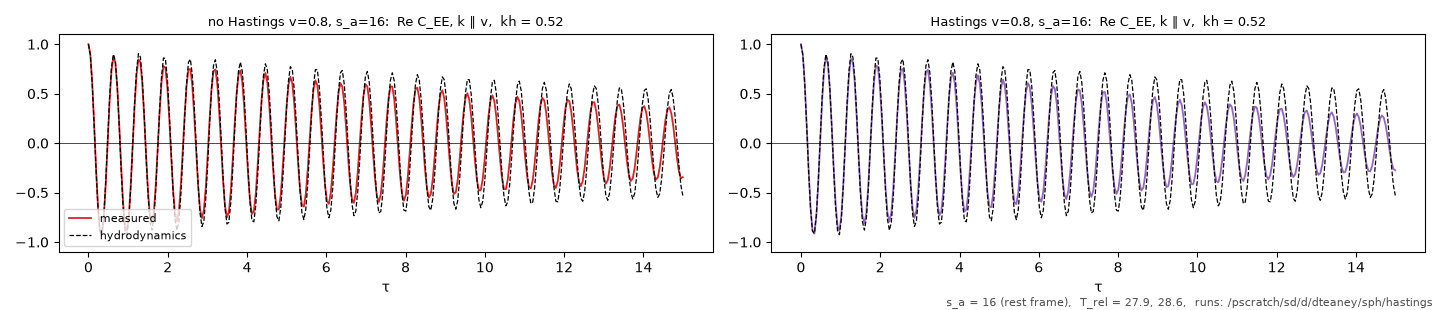
\includegraphics[width=\textwidth]{figs/hastings_nersc_HS16_EEpar_v0.8.png}
\caption{$s_a=16$, $v_0=0.8$: $\mathrm{Re}\,C_{EE}(k\hat x,\tau)$; without (left) and with (right) the correction; dashed hydrodynamics.}
\end{figure}
\begin{figure}[p]
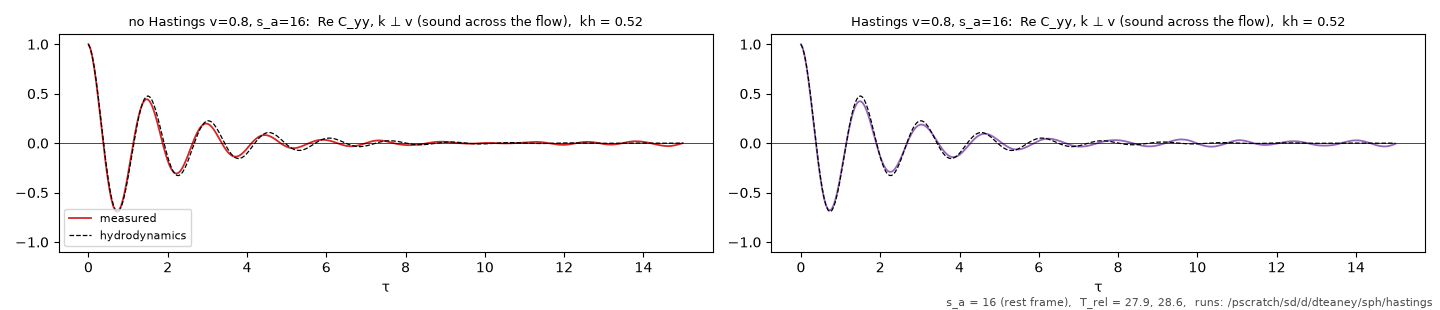
\includegraphics[width=\textwidth]{figs/hastings_nersc_HS16_soundperp_v0.8.png}
\caption{$s_a=16$, $v_0=0.8$: sound across the flow, $\mathrm{Re}\,C_{yy}(k\hat y,\tau)$; without (left) and with (right) the correction; dashed hydrodynamics.}
\end{figure}
\begin{figure}[p]
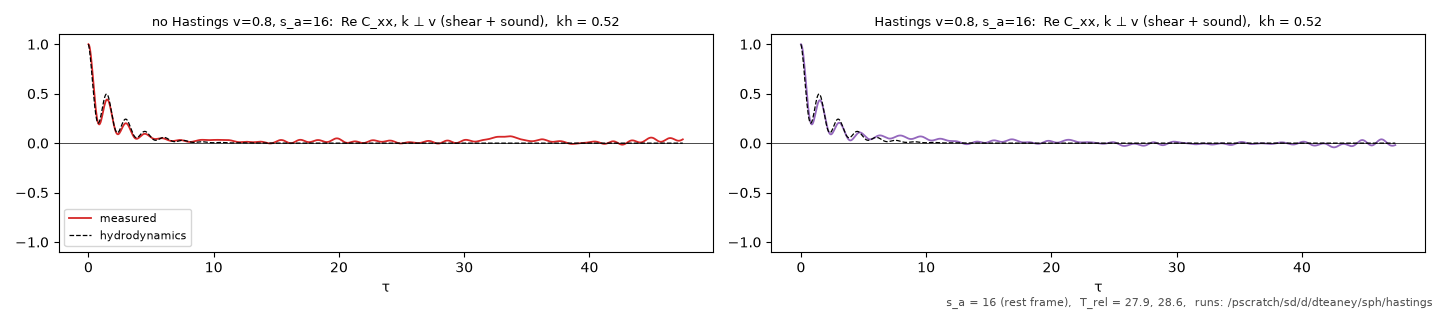
\includegraphics[width=\textwidth]{figs/hastings_nersc_HS16_shearperp_v0.8.png}
\caption{$s_a=16$, $v_0=0.8$: across the flow, $\mathrm{Re}\,C_{xx}(k\hat y,\tau)$ (shear and sound); without (left) and with (right) the correction.}
\label{fig:hs16_last}
\end{figure}

\clearpage
\subsection{Lower entropy per particle: $s_a=12$, $8$ (campaign \texttt{hastings\_low})}
\label{sec:nersc2low}

The same runs at $s_a=12$, $8$ and $4$, with the $\gamma$ cap (\texttt{nersc/campaign\_hastings\_low.txt}, \texttt{77cf74f}; jobs 61376871, 61376872, 61376873, one
packed 4-node job per $s_a$).  $s_a=12$: all 128 runs complete (33 min).  $s_a=8$: all 96 runs of the dynamics complete (34 min); 3 of the 32 HMC
reference chains stopped (below).  $s_a=4$ (37 min): 49 of the 128 tasks stopped, all inside HMC (survivors: at rest 7 without and 10 with the correction, 5 reference chains;
at $v_0=0.8$ 14, 14 and 13); its numbers below are indicative.

\paragraph{A new failure at low $s_a$: the EOS inversion.}  The stopped tasks all end in \texttt{eos\_newton} (\texttt{src/sph.jl:359}): the Newton
iteration for the energy at given entropy and momentum runs away to $e=-\infty$, and \texttt{Trel} takes $\sqrt{-\infty}$ (\texttt{sph.jl:204}).  It
happens inside hybrid Monte Carlo --- the HMC start of the dynamics and the HMC reference chains --- when a leapfrog step takes a particle to a
state the inversion cannot solve.  The $\gamma$ cap gives such states no weight in the entropy, but \texttt{eos\_newton} is called on the
trajectory before the weight is ever evaluated.  The acceptance of the HMC starts that finish is still $0.98$--$0.99$ at every $s_a$ (minimum $0.95$):
the failures are rare single events, not a step size that is too large on average.  Needed: a guard in \texttt{eos\_newton} (no solution $\Rightarrow$
zero weight: the HMC trajectory, or the stochastic proposal, rejected), and perhaps a smaller HMC step at $s_a\le8$.  At $s_a=8$ the reference uses the
surviving chains (14 at rest, 15 at $v_0=0.8$), a small selection.

\paragraph{The trend.}  At rest (the moving fluid shows no bias in either version at any $s_a$, within $2$--$5\%$, \Fig{fig:hs_spectra_low}):
\begin{center}
\resizebox{\textwidth}{!}{\begin{tabular}{lccccc}
\hline
at rest & $s_a=54$ & $16$ & $12$ & $8$ & $4$ \\ \hline
spectra / HMC without the correction ($M_L$, $M_T$, $E$) & $1.02$--$1.08$ & $1.13$--$1.19$ & $1.15$--$1.21$ & $1.05$--$1.12$ & $1.03$--$1.09$ \\
spectra / HMC with the correction & $1.00\pm0.01$ & $0.98$--$1.02$ & $0.94$--$1.02$ & $0.98$--$1.02$ & $0.97$--$1.03$ \\
stress acceptance, without / with & $0.95$ / $0.95$ & $0.92$ / $0.92$ & $0.84$ / $0.85$ & $0.57$ / $0.63$ & $0.22$ / $0.26$ \\
residual acceptance, without / with & $0.66$ / $0.62$ & $0.64$ / $0.44$ & $0.53$ / $0.32$ & $0.23$ / $0.10$ & $0.05$ / $0.008$ \\
light cone, stress / residual (without) & $10^{-6}$ / $10^{-4}$ & $0.03$ / $0.12$ & $0.09$ / $0.28$ & $0.31$ / $0.65$ & $0.65$ / $0.90$ \\
residual $\ln q'/q$, median rms (with) & $1.8$ & $2.1\times10^3$ & $4.8\times10^4$ & $1.1\times10^7$ & --- \\
KE$/2VwT$, without / with & $0.99$ / $0.95$ & $0.97$ / $0.85$ & $0.96$ / $0.82$ & $0.85$ / $0.75$ & $0.65$ / $0.61$ \\
shear $\Gamma/\Gamma_{\rm hydro}$, $kh=0.52$, without / with$^\ddagger$ & $0.92$--$0.99$ / $0.95$--$1.10$ & $0.93$--$0.96$ / $1.04$--$1.08$ & $0.95$--$1.02$ / $1.16$--$1.19$ & $1.49$ / $1.63$--$1.64$ & $2.5$--$2.7$ / $2.6$ \\
$\Delta H/H$ at $t=100$ & $2\times10^{-5}$--$8\times10^{-5}$ & $2\times10^{-3}$ & $4$--$5\times10^{-3}$ & $1\times10^{-2}$ & $0.6$--$1\times10^{-2}$ \\
\hline
\end{tabular}}
\end{center}
\begin{itemize}
\item \emph{With the correction the dynamics matches HMC at every $s_a$}, down to $8$ (one band at $s_a=12$, $kh=0.52$, is $3\sigma$ low).
\item \emph{Without it the excess is largest at $s_a\approx12$--$16$} and smaller again at $8$.  At $s_a=8$ the light cone rejects two thirds of the residual
  and a third of the stress proposals: the stochastic step hardly moves, so its bias has less to act on.
\item \emph{The cost of the correction} grows as $s_a$ falls: the residual acceptance at rest drops by $0.04$, $0.20$, $0.21$, $0.13$ (to $0.10$ at $s_a=8$), and the
  residual log ratios become enormous ($10^7$ at $s_a=8$).
\item \emph{The corrected dynamics damps the shear mode faster at rest} at every $s_a\le16$ (by $0.1$--$0.2$ of $\Gamma_{\rm hydro}$).
\item \emph{$s_a=4$ is beyond the edge.}  At rest the light cone rejects $90\%$ of the residual and $60\%$ of the stress proposals (the step is
  nearly frozen: residual acceptance $0.8\%$ with the correction), the shear mode damps at $2.6$--$2.7\,\Gamma_{\rm hydro}$ in both versions, and KE$/2VwT\approx0.6$.  The
  correction still brings the spectra to HMC, and at $v_0=0.8$ the uncorrected $M_T$ is now biased too ($1.06$--$1.11$, $3$--$7\sigma$; $1$ with the correction).
\item \emph{The method degrades below $s_a\approx12$}: at $s_a=8$ the energy drifts ($\Delta H/H\sim10^{-2}$), the advected shear mode at $v_0=0.8$ moves at
  $\Omega/k=0.77$--$0.78$ instead of $0.80$ (in both versions), and HMC itself begins to fail.
\end{itemize}

\paragraph{The time step that keeps the residual acceptance at a half} (campaign \texttt{dt\_scan}, \texttt{nersc/campaign\_dt\_scan.txt}, job 61379211,
3 debug nodes, 16 min).  Short runs with the correction ($t=5$, $L=0.6$, 2 runs per point) started on the lattice (\texttt{SR\_POSITIONS=lattice}, so that
HMC, which fails at low $s_a$, is not involved), the acceptances averaged over the windows after the lattice has melted ($t>1$).  The time step
factor \texttt{SR\_DTFAC} is halved four times from its campaign value (1 at rest, $0.6$ at $v_0=0.8$); the step itself also depends on the state (its
limit uses the coldest particle), so the steps do not halve exactly.  Residual acceptance with the correction:
\begin{center}
\resizebox{\textwidth}{!}{\begin{tabular}{llcccccc}
\hline
$s_a$ & flow & $1$ & $1/2$ & $1/4$ & $1/8$ & $1/16$ & factor for $\ge1/2$ \\ \hline
$16$ & rest & $0.44$ & $\mathbf{0.61}$ & $0.62$ & $0.74$ & $0.80$ & $1/2$ \\
$16$ & $v_0=0.8$ & $\mathbf{0.57}$ & $0.65$ & $0.74$ & $0.82$ & $0.87$ & $1$ \\
$12$ & rest & $0.28$ & $0.41$ & $\mathbf{0.52}$ & $0.65$ & $0.72$ & $1/4$ \\
$12$ & $v_0=0.8$ & $0.49$ & $\mathbf{0.67}$ & $0.71$ & $0.78$ & $0.88$ & $1/2$ \\
$8$ & rest & $0.12$ & $0.19$ & $0.30$ & $0.38$ & $0.47$ & $\approx1/30$ (extrapolated) \\
$8$ & $v_0=0.8$ & $\mathbf{0.51}$ & $0.56$ & $0.66$ & $0.73$ & $0.78$ & $1$ \\
$4$ & rest & $0.01$ & $0.03$ & $0.05$ & $0.09$ & $0.14$ & out of reach \\
$4$ & $v_0=0.8$ & $0.18$ & $0.27$ & $0.40$ & $0.46$ & $\mathbf{0.51}$ & $1/16$ \\
\hline
\end{tabular}}
\end{center}
The light-cone rejections of the residual proposals fall only slowly with the step: at rest from $8\%$ to $3\%$ ($s_a=16$), $25\%$ to $8\%$ ($12$), $52\%$ to $24\%$
($8$) and $85\%$ to $60\%$ ($4$) between the factors $1$ and $1/16$.  They are mostly a property of the state --- at low $s_a$ a sizeable fraction of the
particles sits close to the light cone, and even small proposals cross it --- not of the step.  So: $s_a=16$ needs half the step (twice the cost),
$s_a=12$ a quarter at rest and a half in the moving fluid (four times the cost), a workable point; $s_a=8$ about $1/30$ at rest, too expensive (in the
moving fluid it is fine as it is); $s_a=4$ is out of reach at rest.  Errors about $\pm0.05$ (two short runs per point).

\begin{figure}[p]
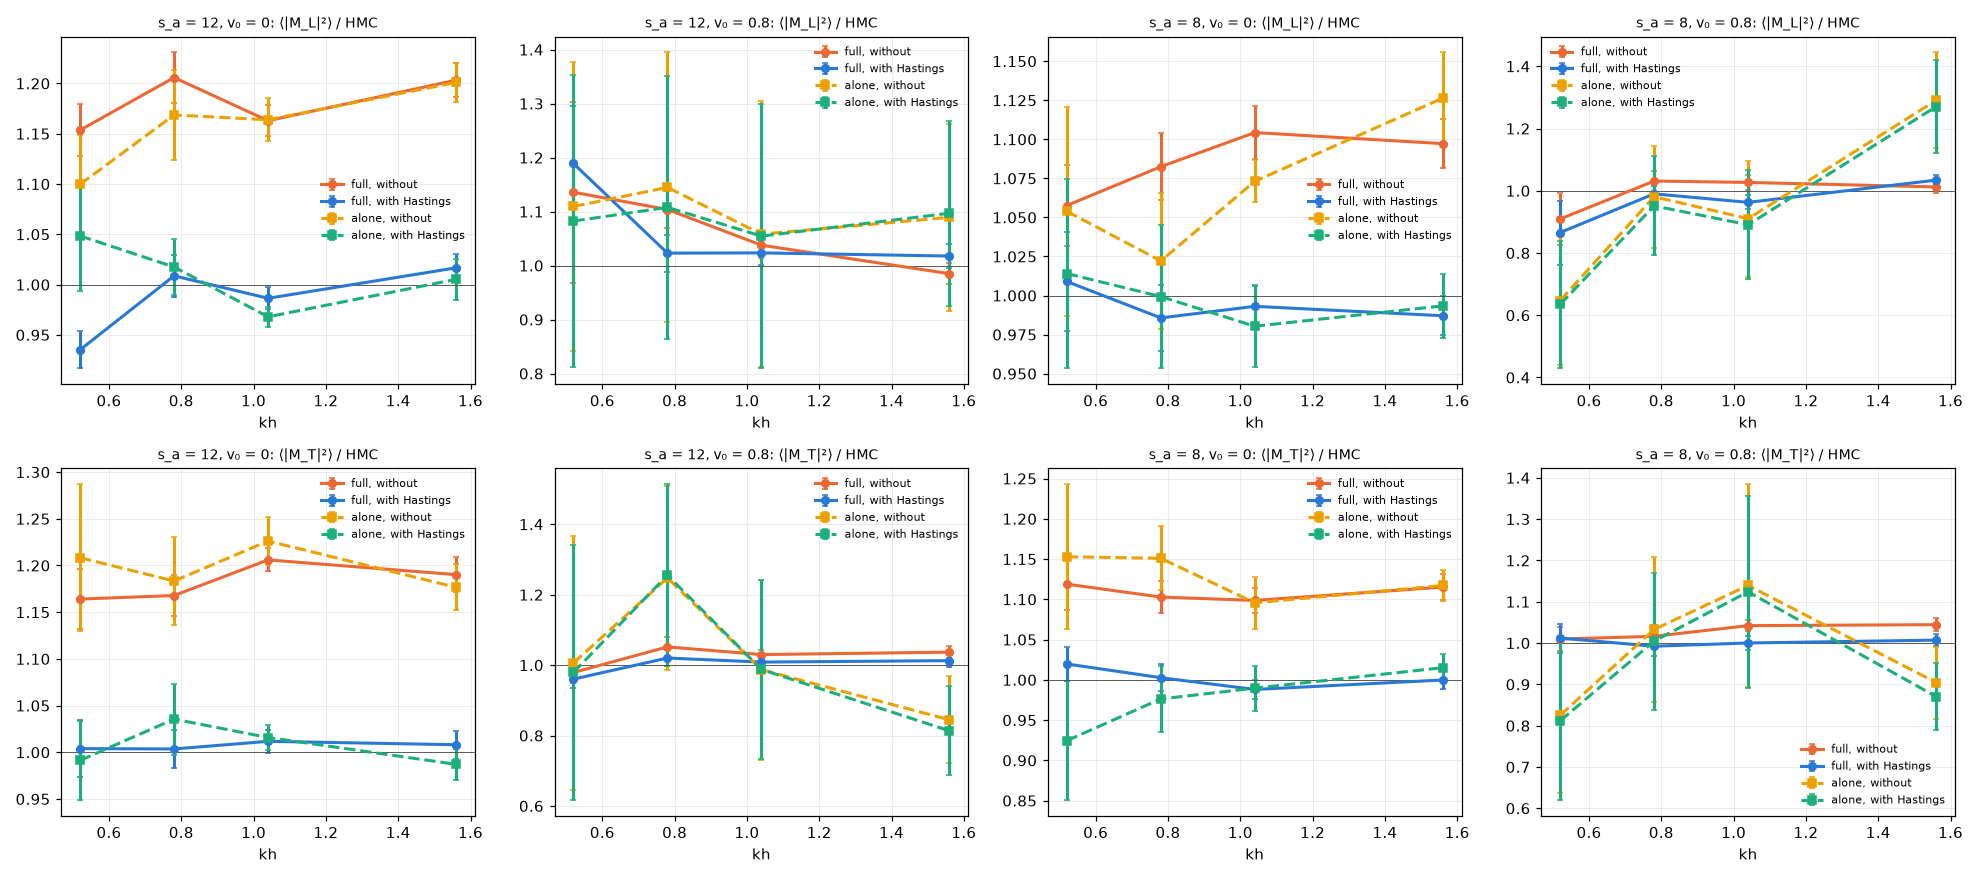
\includegraphics[width=\textwidth]{figs/hastings_nersc_spectra_low.png}
\caption{Campaign \texttt{hastings\_low}: as \Fig{fig:hs_spectra} at $s_a=12$ and $8$ --- the equal-time $\langle|M_L|^2\rangle$, $\langle|M_T|^2\rangle$ of the dynamics over HMC, without (orange) and with (blue) the correction, and the stochastic step alone.}
\label{fig:hs_spectra_low}
\end{figure}
\begin{figure}[p]
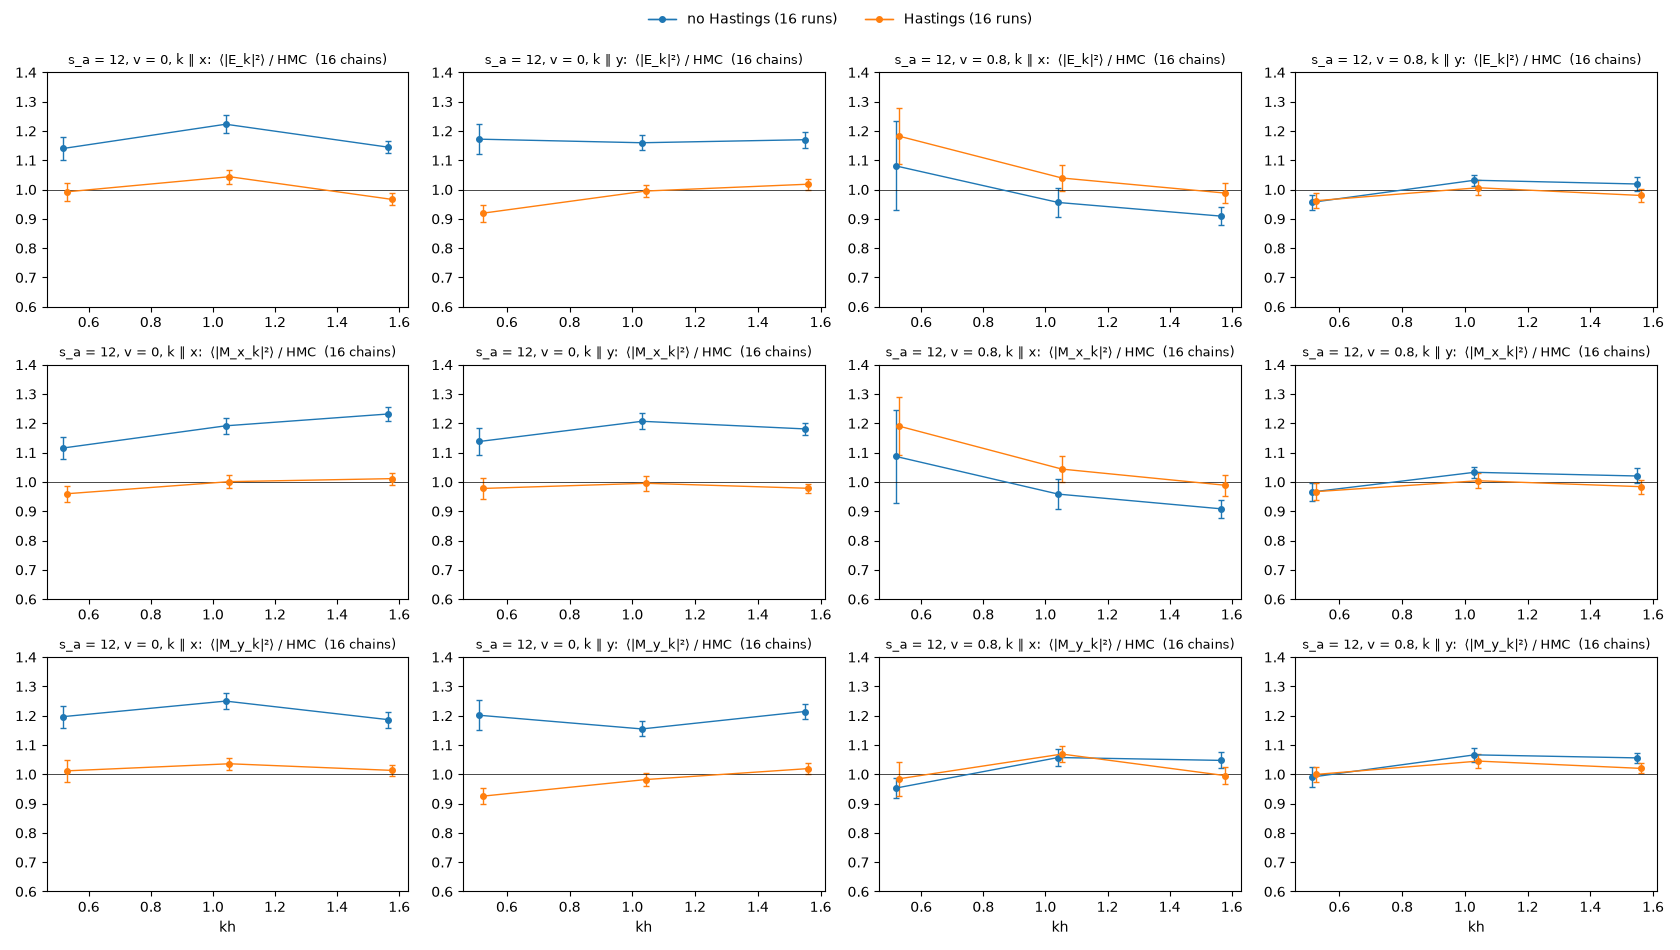
\includegraphics[width=\textwidth]{figs/hastings_nersc_HS12_equaltime_hmc.png}
\caption{$s_a=12$: equal-time $\langle|A_{\bm k}|^2\rangle$ of the dynamics divided by HMC of the same model and measure; without and with the correction (key at the top); 16 runs each.}
\end{figure}
\begin{figure}[p]
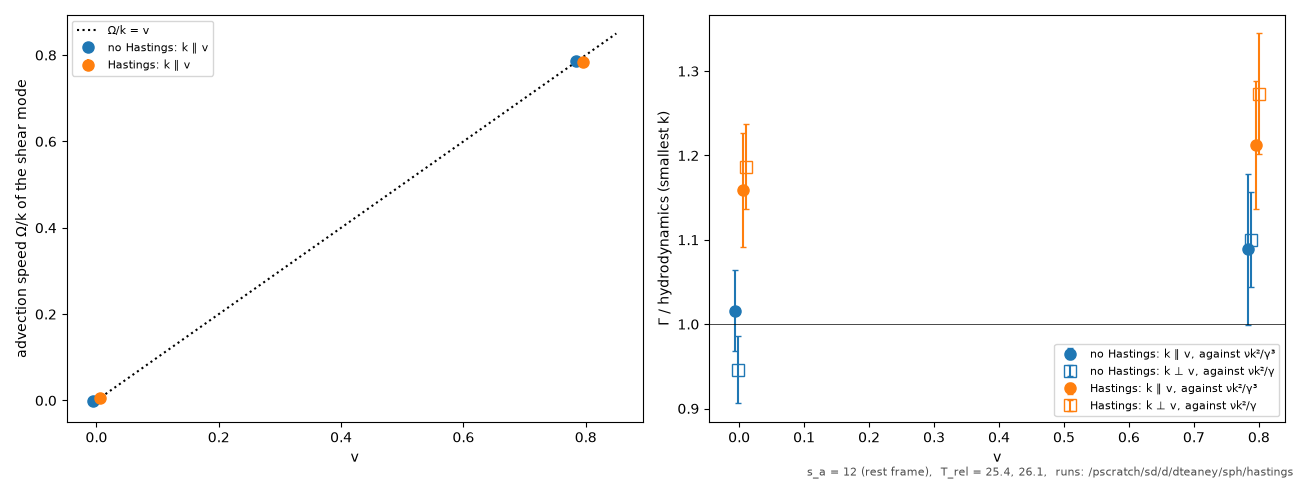
\includegraphics[width=\textwidth]{figs/hastings_nersc_HS12_fit.png}
\caption{$s_a=12$: $\Omega/k$ and $\Gamma/\Gamma_{\rm hydro}$ of the shear mode at $kh=0.52$ against $v_0$, without (blue) and with (orange) the correction; filled along, open across.}
\end{figure}
\begin{figure}[p]
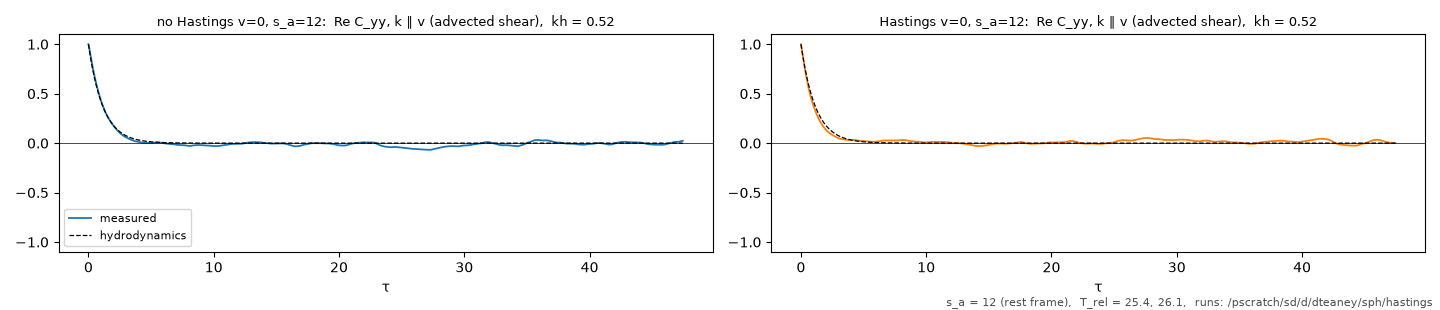
\includegraphics[width=\textwidth]{figs/hastings_nersc_HS12_shear_v0.0.png}
\caption{$s_a=12$, at rest: the shear mode $\mathrm{Re}\,C_{yy}(k\hat x,\tau)$ at $kh=0.52$; without (left) and with (right) the correction; dashed hydrodynamics.}
\end{figure}
\begin{figure}[p]
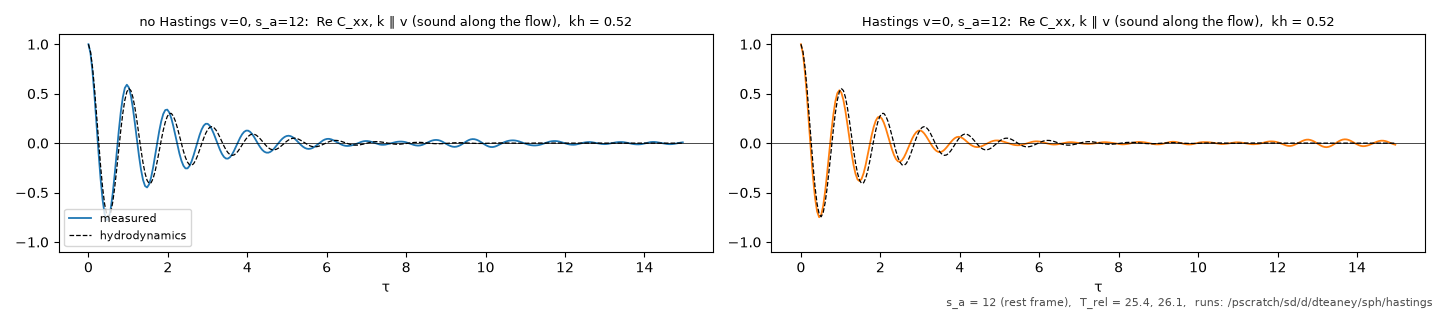
\includegraphics[width=\textwidth]{figs/hastings_nersc_HS12_soundpar_v0.0.png}
\caption{$s_a=12$, at rest: sound, $\mathrm{Re}\,C_{xx}(k\hat x,\tau)$; without (left) and with (right) the correction; dashed hydrodynamics.}
\end{figure}
\begin{figure}[p]
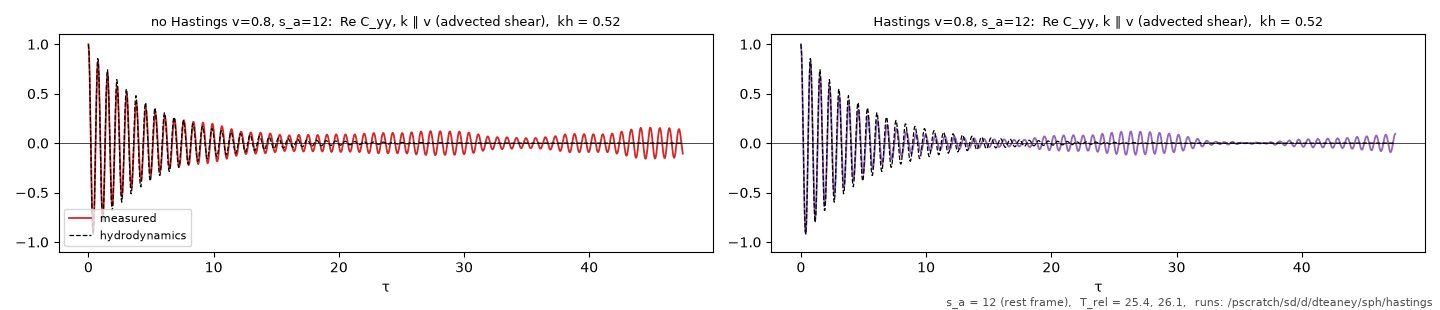
\includegraphics[width=\textwidth]{figs/hastings_nersc_HS12_shear_v0.8.png}
\caption{$s_a=12$, $v_0=0.8$: the advected shear mode $\mathrm{Re}\,C_{yy}(k\hat x,\tau)$; without (left) and with (right) the correction; dashed hydrodynamics.}
\end{figure}
\begin{figure}[p]
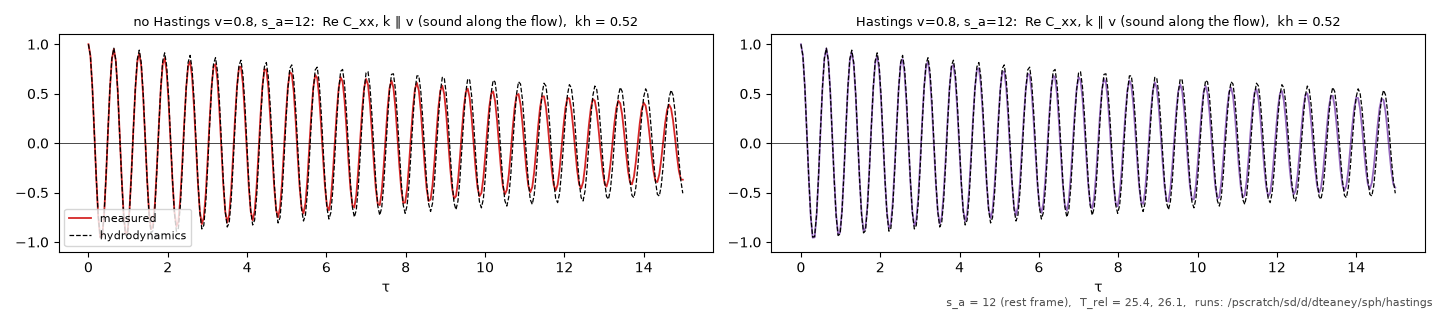
\includegraphics[width=\textwidth]{figs/hastings_nersc_HS12_soundpar_v0.8.png}
\caption{$s_a=12$, $v_0=0.8$: sound along the flow, $\mathrm{Re}\,C_{xx}(k\hat x,\tau)$; without (left) and with (right) the correction; dashed hydrodynamics.}
\end{figure}
\clearpage
\begin{figure}[p]
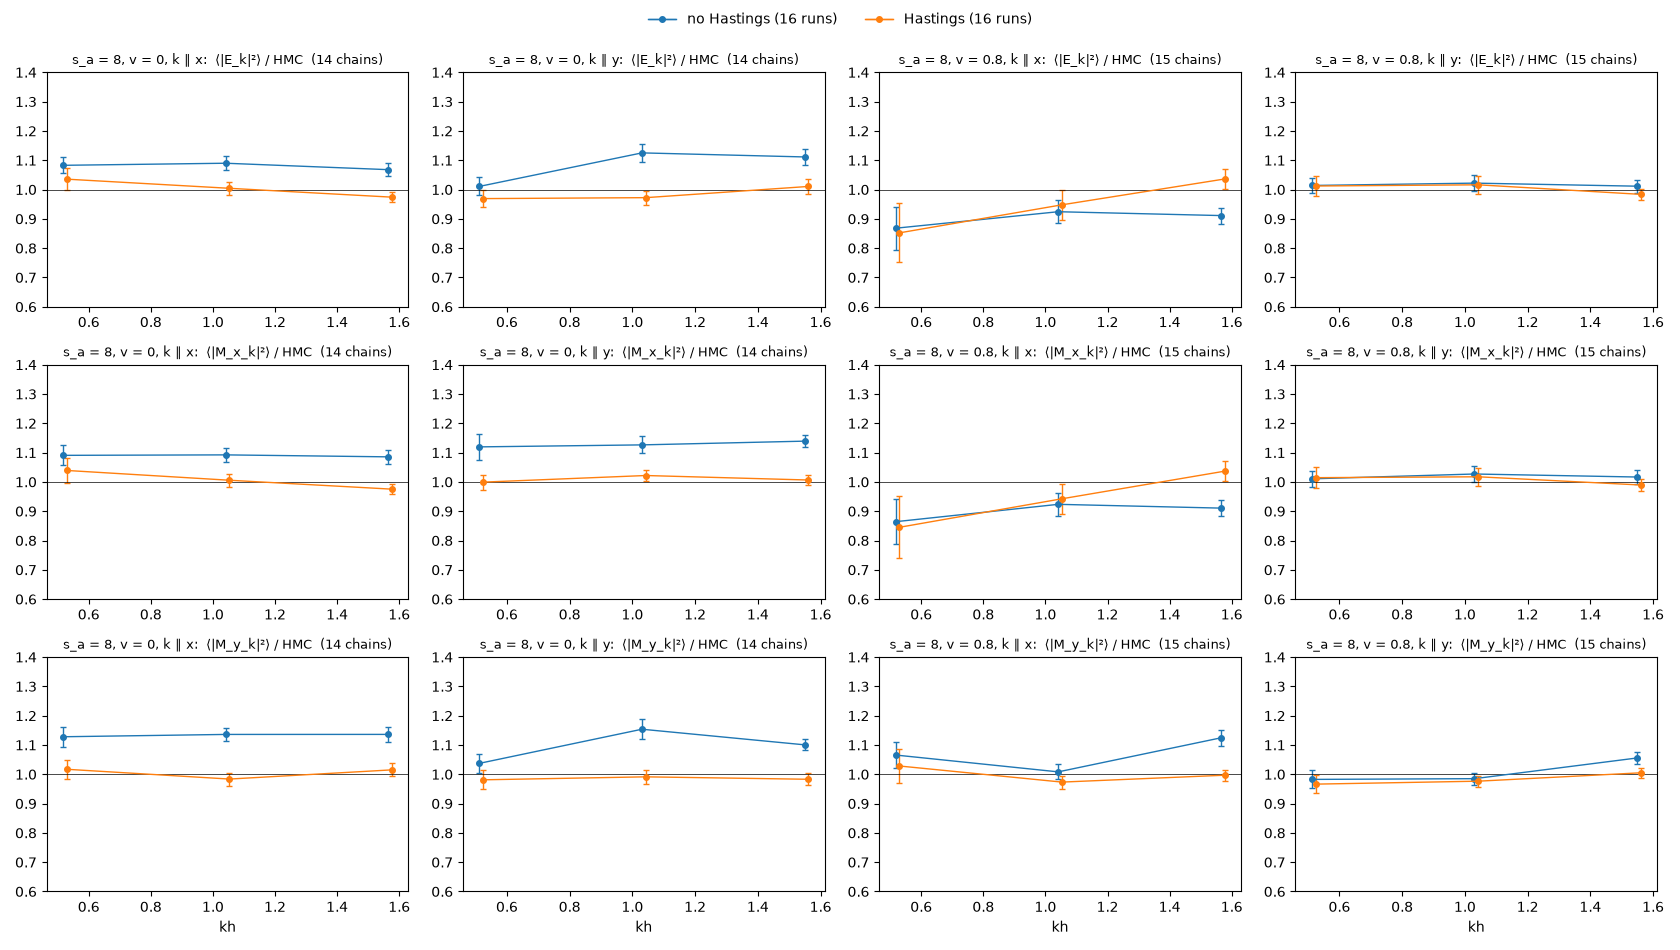
\includegraphics[width=\textwidth]{figs/hastings_nersc_HS8_equaltime_hmc.png}
\caption{$s_a=8$: equal-time $\langle|A_{\bm k}|^2\rangle$ of the dynamics divided by HMC of the same model and measure; without and with the correction (key at the top); 16 runs each.}
\end{figure}
\begin{figure}[p]
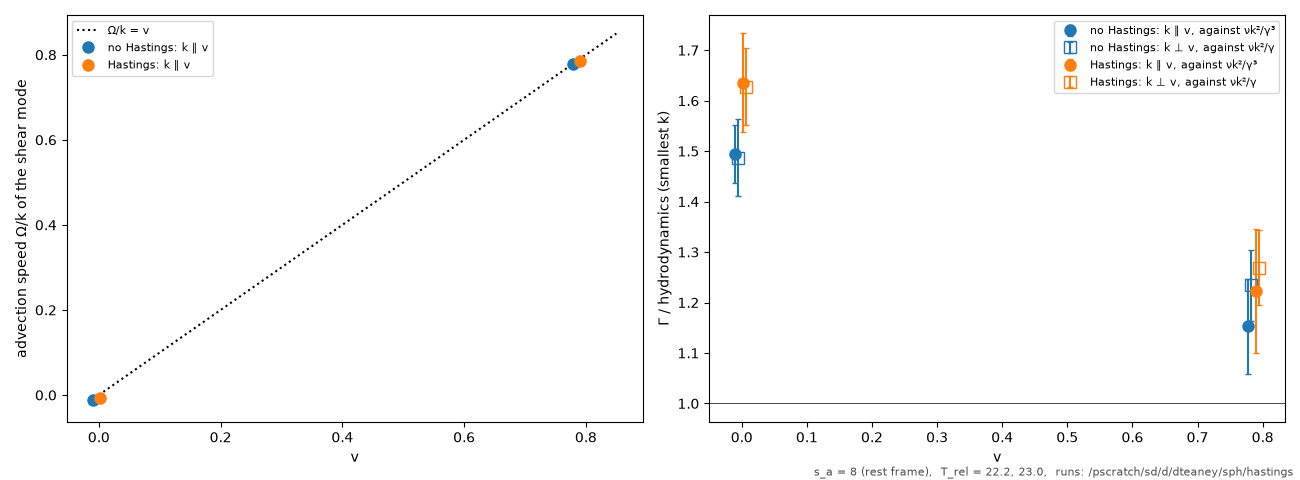
\includegraphics[width=\textwidth]{figs/hastings_nersc_HS8_fit.png}
\caption{$s_a=8$: $\Omega/k$ and $\Gamma/\Gamma_{\rm hydro}$ of the shear mode at $kh=0.52$ against $v_0$, without (blue) and with (orange) the correction; filled along, open across.}
\end{figure}
\begin{figure}[p]
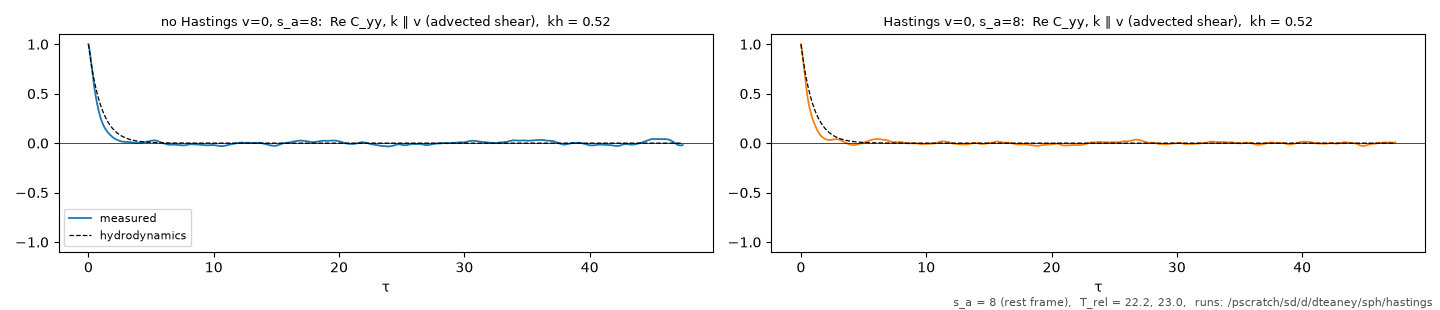
\includegraphics[width=\textwidth]{figs/hastings_nersc_HS8_shear_v0.0.png}
\caption{$s_a=8$, at rest: the shear mode $\mathrm{Re}\,C_{yy}(k\hat x,\tau)$ at $kh=0.52$; without (left) and with (right) the correction; dashed hydrodynamics.}
\end{figure}
\begin{figure}[p]
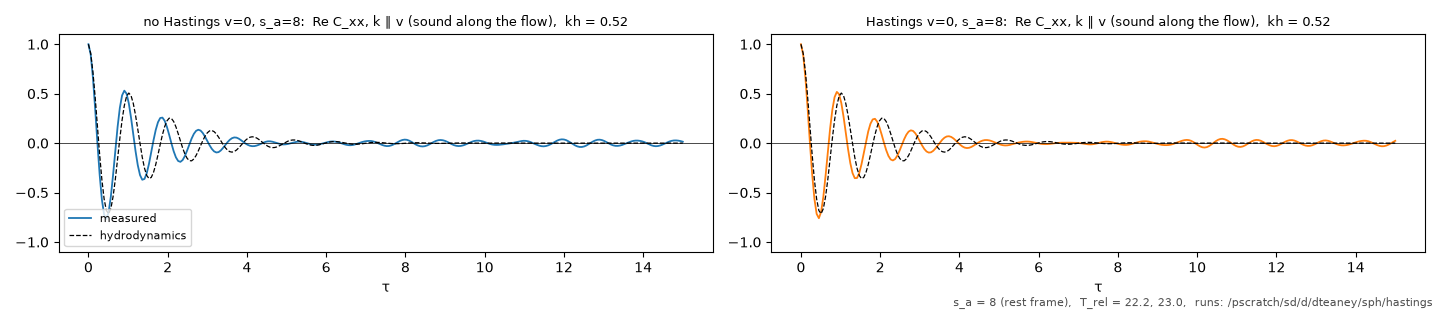
\includegraphics[width=\textwidth]{figs/hastings_nersc_HS8_soundpar_v0.0.png}
\caption{$s_a=8$, at rest: sound, $\mathrm{Re}\,C_{xx}(k\hat x,\tau)$; without (left) and with (right) the correction; dashed hydrodynamics.}
\end{figure}
\begin{figure}[p]
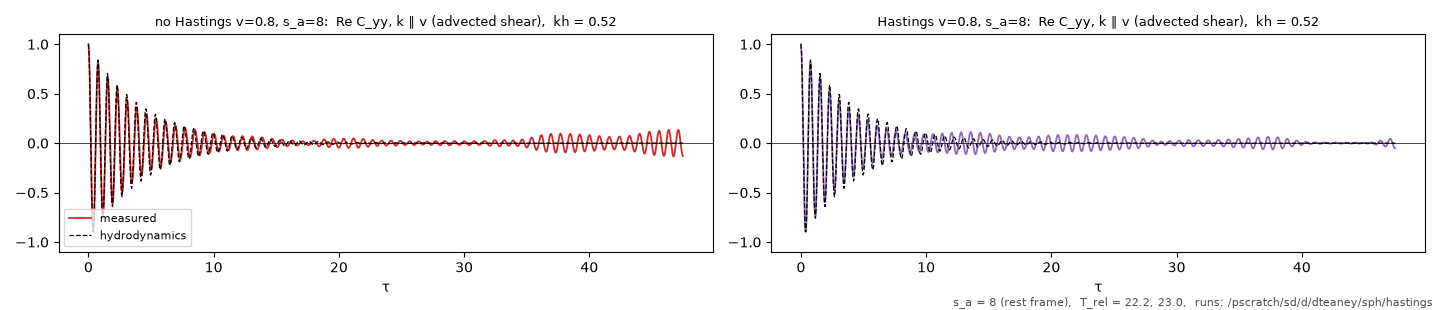
\includegraphics[width=\textwidth]{figs/hastings_nersc_HS8_shear_v0.8.png}
\caption{$s_a=8$, $v_0=0.8$: the advected shear mode $\mathrm{Re}\,C_{yy}(k\hat x,\tau)$; without (left) and with (right) the correction; dashed hydrodynamics.}
\end{figure}
\begin{figure}[p]
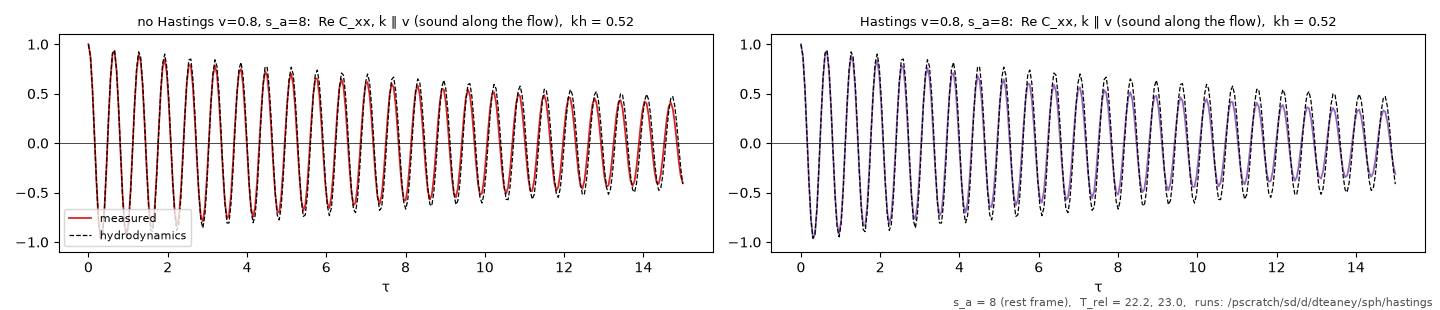
\includegraphics[width=\textwidth]{figs/hastings_nersc_HS8_soundpar_v0.8.png}
\caption{$s_a=8$, $v_0=0.8$: sound along the flow, $\mathrm{Re}\,C_{xx}(k\hat x,\tau)$; without (left) and with (right) the correction; dashed hydrodynamics.}
\end{figure}

\clearpage
\begin{figure}[p]
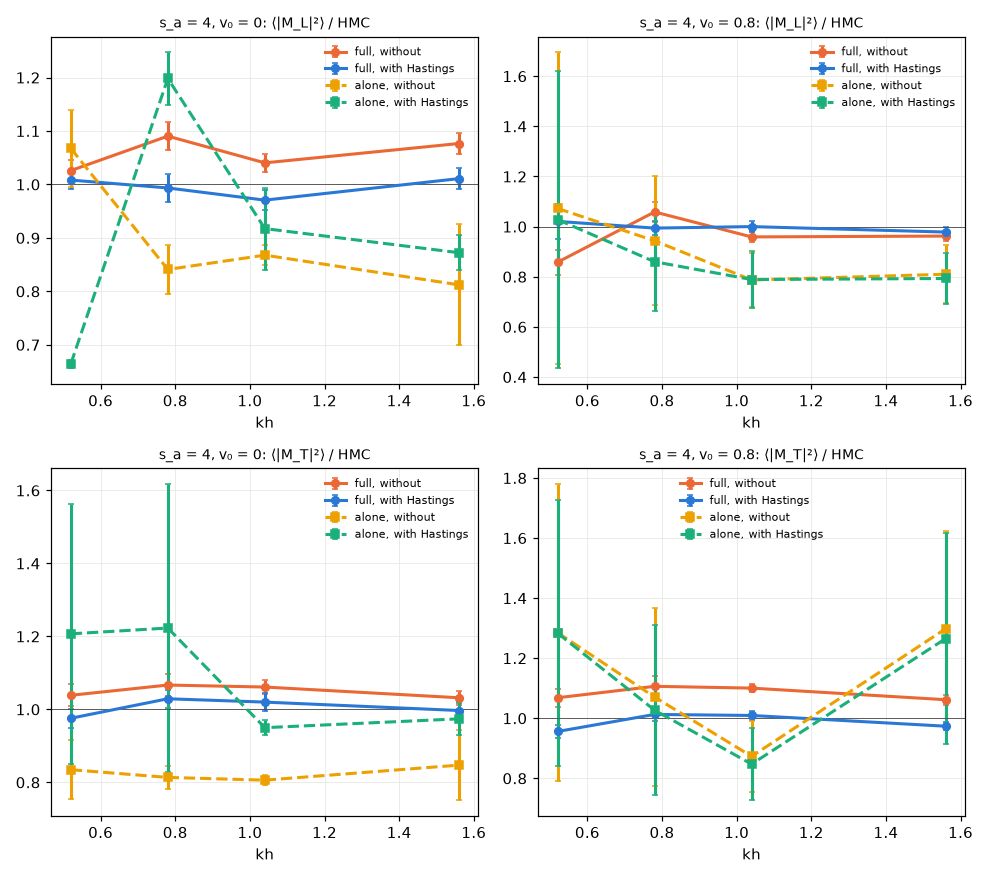
\includegraphics[width=\textwidth]{figs/hastings_nersc_spectra_s4.png}
\caption{$s_a=4$ (survivors; indicative): the equal-time $\langle|M_L|^2\rangle$, $\langle|M_T|^2\rangle$ of the dynamics over HMC (5 chains at rest, 13 at $v_0=0.8$), without (orange) and with (blue) the correction, and the stochastic step alone.}
\end{figure}
\begin{figure}[p]
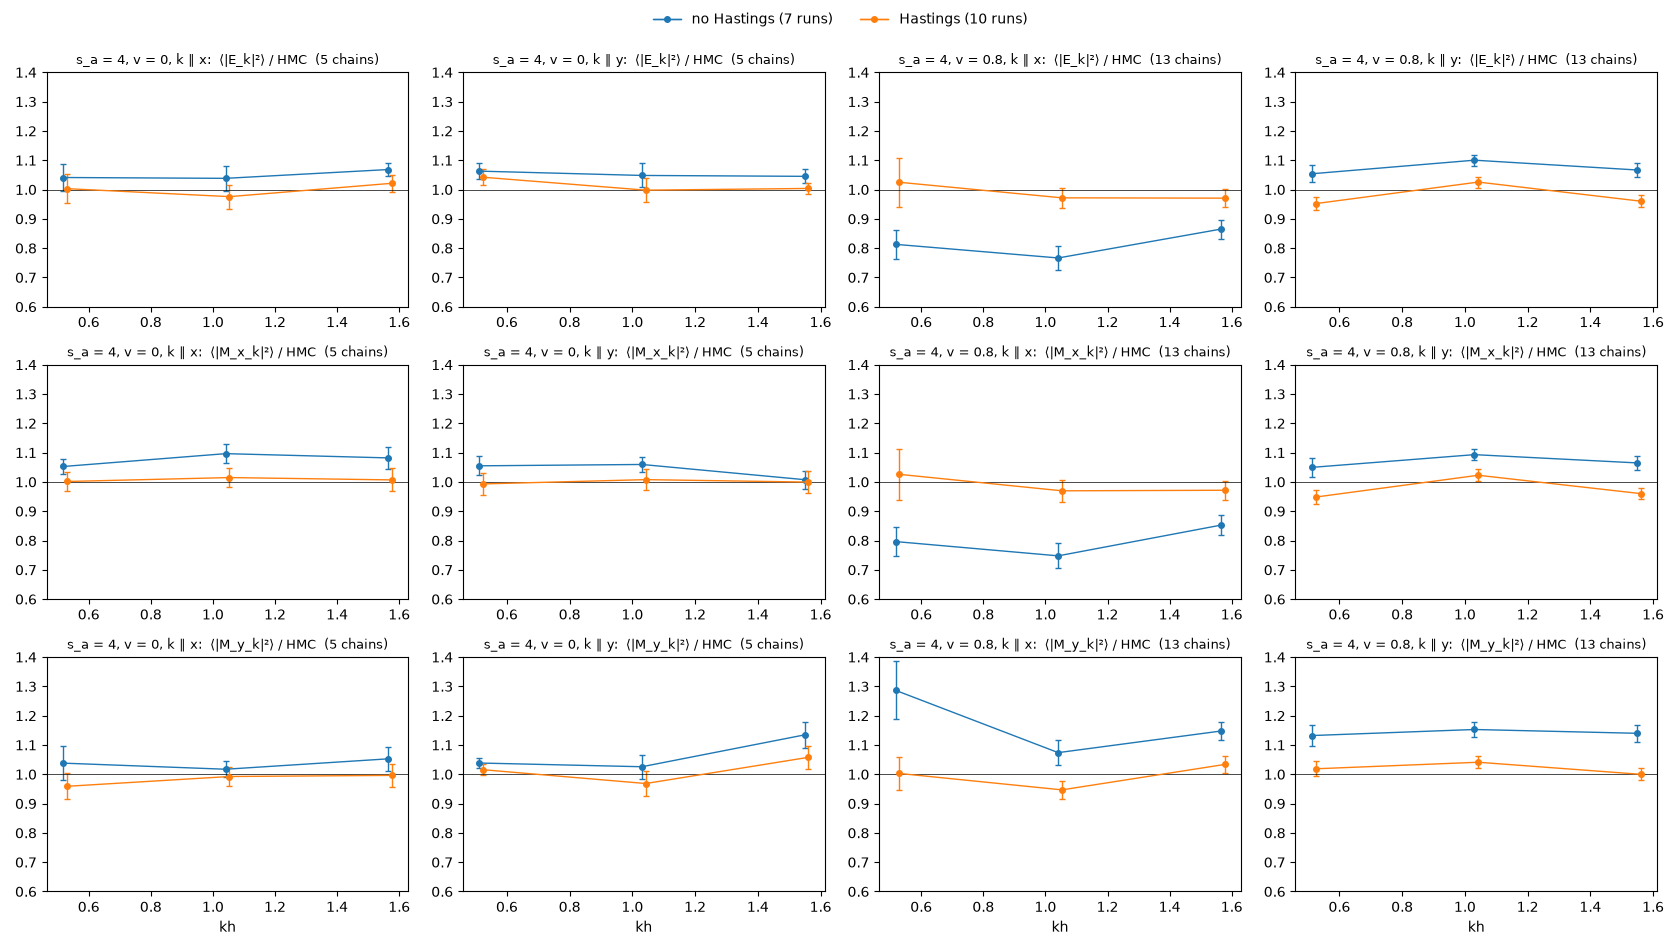
\includegraphics[width=\textwidth]{figs/hastings_nersc_HS4_equaltime_hmc.png}
\caption{$s_a=4$: equal-time $\langle|A_{\bm k}|^2\rangle$ divided by HMC, without (7 runs at rest, 14 moving) and with (10, 14) the correction.}
\end{figure}
\begin{figure}[p]
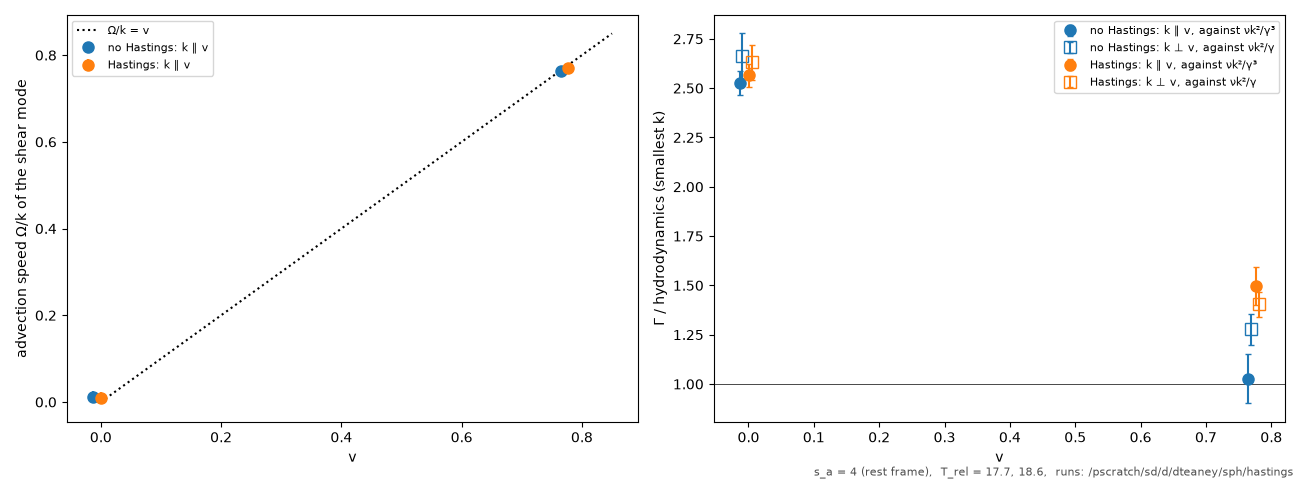
\includegraphics[width=\textwidth]{figs/hastings_nersc_HS4_fit.png}
\caption{$s_a=4$: $\Omega/k$ and $\Gamma/\Gamma_{\rm hydro}$ of the shear mode at $kh=0.52$ against $v_0$, without (blue) and with (orange) the correction; filled along, open across.}
\end{figure}
\begin{figure}[p]
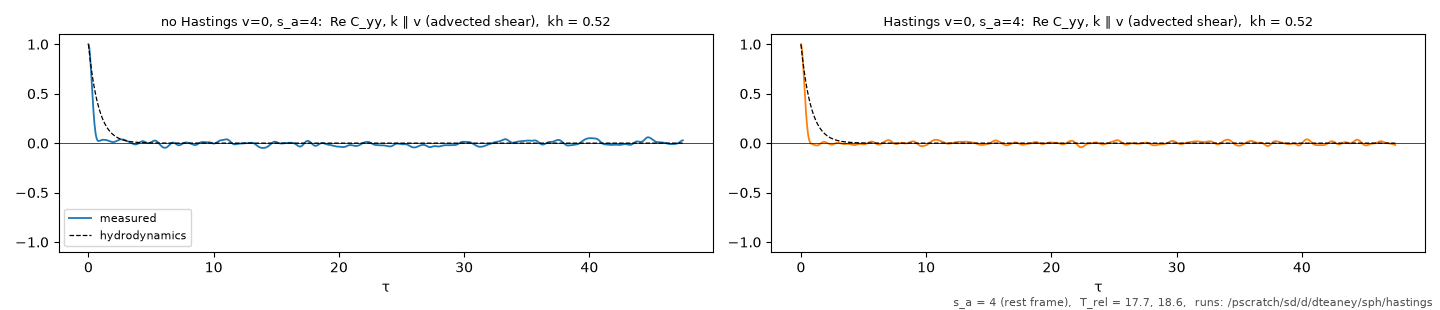
\includegraphics[width=\textwidth]{figs/hastings_nersc_HS4_shear_v0.0.png}
\caption{$s_a=4$, at rest: the shear mode $\mathrm{Re}\,C_{yy}(k\hat x,\tau)$ at $kh=0.52$, without (left) and with (right) the correction: $2.6$--$2.7$ times faster than hydrodynamics (dashed).}
\end{figure}
\begin{figure}[p]
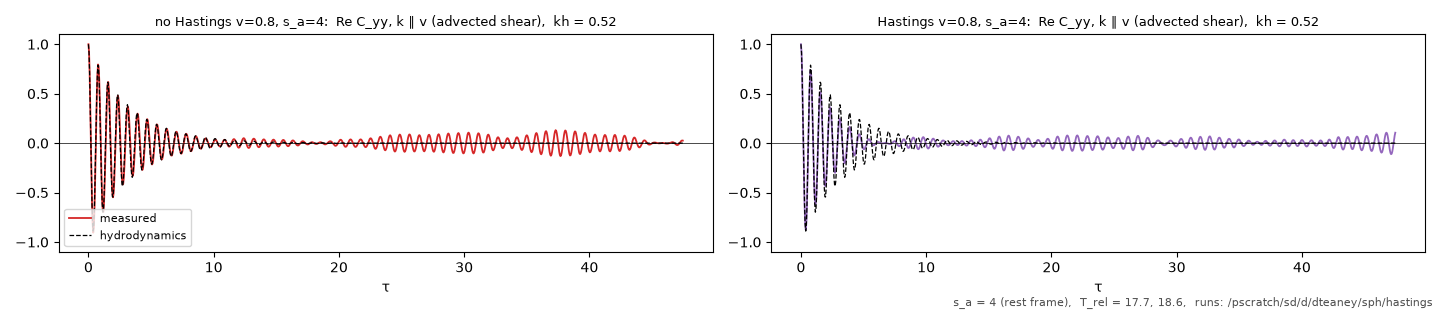
\includegraphics[width=\textwidth]{figs/hastings_nersc_HS4_shear_v0.8.png}
\caption{$s_a=4$, $v_0=0.8$: the advected shear mode, without (left) and with (right) the correction; dashed hydrodynamics.}
\end{figure}


%=============================================================================
\section{Correction of the analysis: runs with different time steps (2026-11-26)}
\label{sec:lagfix}

The time step of a run is set at its start, from the initial state, so at $s_a\le16$ the runs of one set do not share a step; in campaign
\texttt{hastings} nearly every run has its own.  \texttt{examples/boost\_analysis.jl} correlated each run on its own lag grid but averaged the runs on
the grid of the first one, so every run with another step was put on a compressed or stretched time axis (found in \nolinkurl{split_dynamics.tex},
``Correction of the analysis'').  Since 2026-11-26 every run is put on the grid of the most common lag spacing (a run with another spacing is
correlated at every record and interpolated); sets whose runs share one step are unchanged, so $s_a=54$ is as before.  The groups HS16, HS12, HS8 and HS4
were analysed again with the old and the corrected script, and the figures of this note at those $s_a$ are now the corrected ones.  The shear damping
$\Gamma/\Gamma_{\rm hydro}$, old $\to$ corrected (the error in the last digits):
\begin{center}
\resizebox{\textwidth}{!}{\begin{tabular}{lcccccccc}
\hline
 & \multicolumn{4}{c}{at rest} & \multicolumn{4}{c}{$v_0=0.8$} \\
$s_a$ & $kh=0.52$, $x$ & $kh=0.52$, $y$ & $kh=1.05$, $x$ & $kh=1.05$, $y$ & $0.52$, along & $0.52$, across & $1.05$, along & $1.05$, across \\
\hline
\multicolumn{9}{l}{without the correction (no Hastings factor)} \\
$16$ & 1.05(6)$\to$0.93(4) & 1.08(7)$\to$0.96(5) & 1.08(4)$\to$0.96(3) & 1.01(4)$\to$0.90(2) & 2.52(55)$\to$1.02(15) & 1.28(8)$\to$1.25(7) & 1.61(17)$\to$1.17(7) & 1.17(4)$\to$1.18(4) \\
$12$ & 0.98(4)$\to$1.02(5) & 0.92(4)$\to$0.95(4) & 0.94(2)$\to$0.96(1) & 0.87(4)$\to$0.89(3) & 2.27(32)$\to$1.09(9) & 1.11(6)$\to$1.10(6) & 1.48(11)$\to$1.19(6) & 1.09(5)$\to$1.06(4) \\
$8$ & 1.24(8)$\to$1.49(6) & 1.25(7)$\to$1.49(8) & 0.97(6)$\to$1.18(2) & 0.99(5)$\to$1.21(4) & 1.46(10)$\to$1.15(9) & 1.22(7)$\to$1.23(7) & 1.25(4)$\to$1.20(4) & 1.02(3)$\to$1.04(4) \\
$4$ & 2.63(6)$\to$2.53(6) & 2.76(14)$\to$2.66(12) & 1.57(4)$\to$1.51(4) & 1.47(6)$\to$1.42(5) & 1.35(9)$\to$1.03(12) & 1.34(8)$\to$1.28(8) & 1.19(5)$\to$1.09(4) & 0.96(3)$\to$0.90(2) \\
\hline
\multicolumn{9}{l}{with the correction} \\
$16$ & 1.22(8)$\to$1.08(6) & 1.17(7)$\to$1.04(5) & 1.23(5)$\to$1.10(3) & 1.17(4)$\to$1.04(3) & 2.34(48)$\to$1.06(10) & 1.25(10)$\to$1.22(9) & 1.64(20)$\to$1.11(5) & 1.10(3)$\to$1.07(3) \\
$12$ & 1.13(6)$\to$1.16(7) & 1.15(6)$\to$1.19(5) & 1.07(4)$\to$1.10(2) & 1.03(4)$\to$1.06(2) & 1.97(29)$\to$1.21(8) & 1.30(8)$\to$1.27(7) & 1.51(11)$\to$1.18(6) & 1.06(3)$\to$1.06(3) \\
$8$ & 1.35(8)$\to$1.64(10) & 1.36(10)$\to$1.63(8) & 1.04(6)$\to$1.27(2) & 1.07(7)$\to$1.30(3) & 1.53(17)$\to$1.22(12) & 1.25(7)$\to$1.27(7) & 1.18(5)$\to$1.09(4) & 0.96(2)$\to$0.97(2) \\
$4$ & 2.66(7)$\to$2.57(6) & 2.73(10)$\to$2.63(9) & 1.37(4)$\to$1.32(4) & 1.47(5)$\to$1.41(5) & 1.75(14)$\to$1.50(10) & 1.46(7)$\to$1.40(6) & 1.30(5)$\to$1.21(4) & 0.91(4)$\to$0.85(3) \\
\hline
\end{tabular}}
\end{center}
\begin{itemize}
\item \emph{In motion along the flow} the old analysis over-stated the damping at $kh=0.52$: $2.3$--$2.5\to1.0$--$1.1$ at $s_a=16$, $2.0$--$2.3\to1.1$--$1.2$ at
  $s_a=12$.  The ``limit of the dynamics at this entropy per particle'' of the first version of this note is gone: in motion the damping is within
  $1.0$--$1.3$ of hydrodynamics down to $s_a=8$.
\item \emph{At rest} the corrections are of $0.1$ to $0.25$, of either sign: down at $s_a=16$, up at $s_a=8$ (where the first run had a larger step).  The
  difference between the corrected and the uncorrected dynamics, $+0.1$ to $+0.15$ of $\Gamma_{\rm hydro}$ at rest, stays.
\item \emph{$s_a=4$} changes least at rest ($2.5$--$2.7$); it remains beyond the edge.
\end{itemize}
The rows of the tables above that are marked $^\ddagger$ carry the corrected values; the text of the earlier sections, where it quotes the damping in
motion at $s_a\le16$, refers to the old ones.

\end{document}
